\chapter{Actors, Actions and Workflow Overview}\label{ch:1}

This document presents the workflows of the \emph{AI Legal Advisor and Analyzer} from the point of view of each actor. For every actor it lists the actions the actor can perform, the dependencies each action has on other actors or on system state, and a workflow (activity) diagram for every workflow the actor takes part in. It extends the use cases (UC-01 to UC-12) and functional requirements (UFR, LFR, AFR) of Chapter 3 of the project report. All workflows describe the planned system.

\needspace{12\baselineskip}
\section{Actors}

\begin{center}
\begin{tabular}{|L{2.23cm}|L{1.70cm}|L{1.70cm}|L{8.38cm}|}
\hline\headrow \thd{Actor} & \thd{Type} & \thd{Portal} & \thd{Responsibility} \\ \hline
\textbf{User (Citizen)} & Primary & User portal & Describes legal problems, receives grounded guidance, uploads evidence, finds lawyers, requests consultations and tracks cases. \\ \hline
\textbf{Lawyer} & Primary & Lawyer portal & Maintains a verified public profile, handles consultation requests, works on shared cases and posts updates. \\ \hline
\textbf{Admin} & Primary & Admin portal & Verifies lawyers, controls the legal knowledge base, manages accounts, moderates content and monitors activity. \\ \hline
\textbf{AI Services (System)} & Secondary & None (backend) & Embedding model, Qdrant retrieval, open-source LLM, citation checker, PyMuPDF and OCR that execute the automated steps. \\ \hline
\textbf{Email / Notification Service} & Secondary & None (backend) & Sends verification, password-reset and status notifications. \\ \hline
\end{tabular}
\end{center}

\needspace{12\baselineskip}
\section{Diagram Notation}

All workflow diagrams use the same notation:

\begin{itemize}
  \item \textbf{Rounded box:} start or end of a workflow.
  \item \textbf{Rectangle:} an action performed by the actor or the system.
  \item \textbf{Hexagon:} a decision or check (labelled exits such as Yes and No).
  \item \textbf{Solid arrow:} the normal flow of control.
  \item \textbf{Dashed arrow:} a dependency on another actor's workflow or on system state.
  \item \textbf{Coloured lanes:} in swimlane diagrams, which actor performs each step.
\end{itemize}

Each workflow is labelled with an identifier (for example U-WF2). Each action is labelled with an identifier (for example U-A05) that is used in the action tables and the dependency analysis.

\needspace{12\baselineskip}
\section{Workflow Summary}

\begin{longtable}{|L{1.70cm}|L{6.75cm}|L{1.70cm}|L{1.70cm}|L{1.70cm}|}
\caption{Workflows by actor}\label{tab:1.1}\\
\hline\headrow \thd{Workflow ID} & \thd{Workflow} & \thd{Actor} & \thd{Related use case} & \thd{Section} \\ \hline
\endfirsthead
\hline\headrow \thd{Workflow ID} & \thd{Workflow} & \thd{Actor} & \thd{Related use case} & \thd{Section} \\ \hline
\endhead
\hline\endlastfoot
U-WF1 & Account access and profile management & User & UC-01 & 2.2 \\ \hline
U-WF2 & Create case and clarify facts & User & UC-02 & 2.3 \\ \hline
U-WF3 & Obtain AI legal guidance & User & UC-03 & 2.4 \\ \hline
U-WF4 & Upload documents and complete evidence checklist & User & UC-04 & 2.5 \\ \hline
U-WF5 & Find a lawyer and request a consultation & User & UC-05, UC-06 & 2.6 \\ \hline
U-WF6 & Track case, communicate and review & User & UC-07 & 2.7 \\ \hline
L-WF1 & Registration and verification & Lawyer & UC-01, UC-08 & 3.2 \\ \hline
L-WF2 & Public profile and availability management & Lawyer & UC-08 & 3.3 \\ \hline
L-WF3 & Handle consultation requests & Lawyer & UC-09 & 3.4 \\ \hline
L-WF4 & Work on a shared case & Lawyer & UC-09 & 3.5 \\ \hline
A-WF1 & Lawyer verification & Admin & UC-10 & 4.2 \\ \hline
A-WF2 & Legal knowledge base management & Admin & UC-11 & 4.3 \\ \hline
A-WF3 & User and lawyer account management & Admin & UC-12 & 4.4 \\ \hline
A-WF4 & Content moderation & Admin & UC-12 & 4.5 \\ \hline
A-WF5 & Monitoring and audit & Admin & UC-12 & 4.6 \\ \hline
S-WF1 & RAG guidance pipeline & AI Services & UC-03 & 5.1 \\ \hline
S-WF2 & Document processing pipeline & AI Services & UC-04 & 5.2 \\ \hline
S-WF3 & Knowledge base ingestion pipeline & AI Services & UC-11 & 5.3 \\ \hline
S-WF4 & Notification dispatch & Notification Service & UC-06, UC-09 & 5.4 \\
\end{longtable}

\section{End-to-End Workflow Across Actors}

Figure~\ref{fig:1.1} shows the complete journey of one case across all actors in swimlanes. It also shows the two preconditions that the Admin must satisfy before the citizen's journey can succeed: a verified knowledge base and verified lawyers.

% Mermaid source:
% %% name: e2e_swimlane
% flowchart TB
%     subgraph ADM["Admin"]
%         direction LR
%         A1["Add and verify legal sources"] ~~~ A2["Verify lawyer credentials"]
%     end
%     subgraph LAW["Lawyer"]
%         direction LR
%         L1(["Register and submit licence"]) --> L2["Build public profile"]
%         L3["Review request and shared case"] --> L4["Accept and schedule"] --> L5["Post updates and messages"] --> L6["Complete consultation"]
%     end
%     subgraph SYS["AI Services (System)"]
%         direction LR
%         S1["Classify area and topic"] --> S2["Find missing facts"]
%         S3["Retrieve law, generate answer, check citations"]
%         S4["Extract text and clauses, update checklist"]
%         S5["Notify participants"]
%     end
%     subgraph USR["User (Citizen)"]
%         direction LR
%         U1(["Register and log in"]) --> U2["Describe problem"] --> U3["Answer follow-up questions"] --> U4["Read guidance and sources"] --> U5["Upload documents"] --> U6["Search verified lawyers"] --> U7["Request consultation and consent"] --> U8["Track case timeline"] --> U9(["Mark resolved and review"])
%     end
%     U2 --> S1
%     S2 --> U3
%     U3 --> S3 --> U4
%     U5 --> S4
%     U7 --> S5 --> L3
%     L5 --> U8
%     L6 --> U9
%     L1 --> A2 --> L2
%     A1 -.->|"knowledge base ready"| S3
%     L2 -.->|"verified profile listed"| U6
\begin{figure}[H]\centering
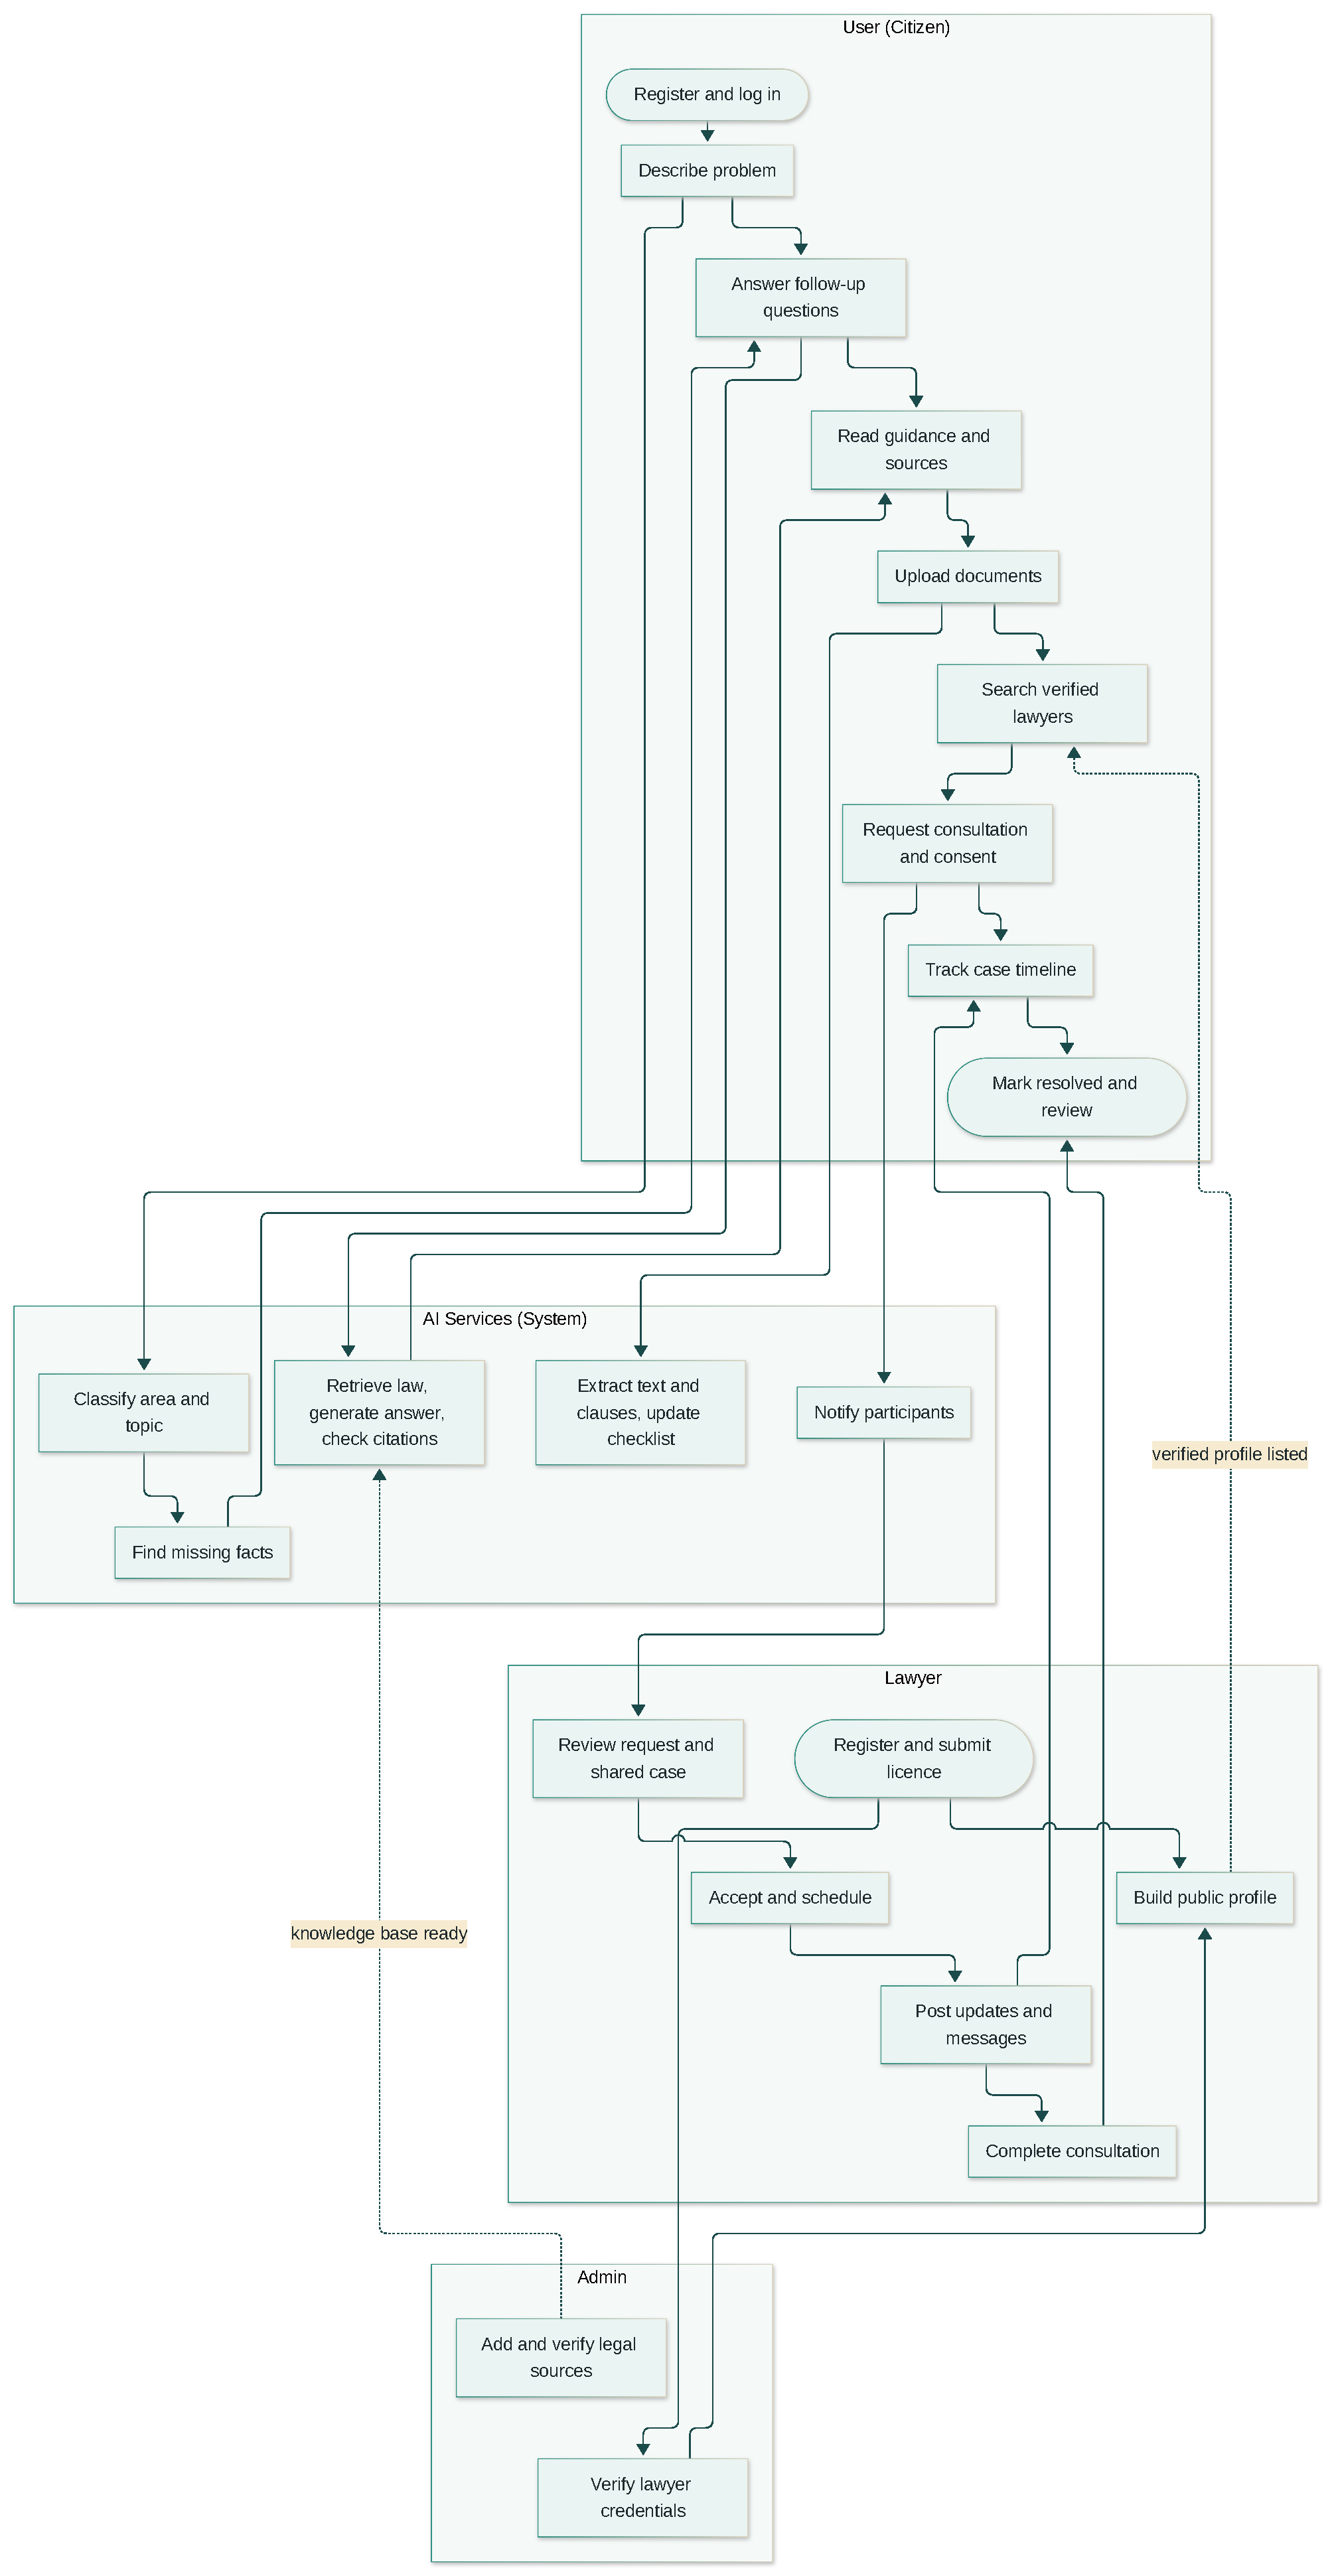
\includegraphics[width=\textwidth,height=0.80\textheight,keepaspectratio]{figures/e2e_swimlane.pdf}
\caption{End-to-end swimlane workflow across all actors}\label{fig:1.1}
\end{figure}

\needspace{12\baselineskip}
\section{Actor-Action Matrix}

Table~\ref{tab:1.2} summarises which actor can perform each group of actions. Detailed action catalogues with dependencies follow in Chapters 2 to 5.

\begin{longtable}{|L{6.68cm}|L{1.70cm}|L{1.60cm}|L{1.70cm}|L{1.87cm}|}
\caption{Actor-action matrix}\label{tab:1.2}\\
\hline\headrow \thd{Action group} & \thd{User} & \thd{Lawyer} & \thd{Admin} & \thd{AI Services} \\ \hline
\endfirsthead
\hline\headrow \thd{Action group} & \thd{User} & \thd{Lawyer} & \thd{Admin} & \thd{AI Services} \\ \hline
\endhead
\hline\endlastfoot
Register, log in, reset password & Yes & Yes & Log in only & No \\ \hline
Manage own profile & Personal profile & Public professional profile & No & No \\ \hline
Create and manage cases & Yes & No & View for moderation & No \\ \hline
Answer follow-up questions & Yes & No & No & Generates questions \\ \hline
Request AI legal guidance & Yes & No & No & Executes RAG pipeline \\ \hline
Upload documents & Yes & No & No & Extracts text and clauses \\ \hline
Search lawyers and view public profiles & Yes & No & Yes & No \\ \hline
Request consultation, give or revoke consent & Yes & No & No & No \\ \hline
Accept, decline or schedule consultations & No & Yes & No & No \\ \hline
View shared case & Owner & With active consent & Moderation only & No \\ \hline
Message within consultation & Yes & Yes & No & No \\ \hline
Post case status updates & Mark resolved or closed & Yes & No & System events \\ \hline
Rate and review lawyer & Yes & No & Moderate & No \\ \hline
Verify lawyers & No & Submits request & Yes & No \\ \hline
Manage legal knowledge base & No & No & Yes & Indexes sources \\ \hline
Suspend or reactivate accounts & No & No & Yes & No \\ \hline
View statistics and audit log & No & Own dashboard & Yes & No \\
\end{longtable}

\chapter{User (Citizen) Workflows}\label{ch:2}

\section{User Actions and Dependencies}

\begin{longtable}{|L{2.06cm}|L{3.43cm}|L{2.92cm}|L{3.43cm}|L{1.70cm}|}
\caption{Actions of the User and their dependencies}\label{tab:2.1}\\
\hline\headrow \thd{ID} & \thd{Action} & \thd{Depends on} & \thd{Result} & \thd{Req.} \\ \hline
\endfirsthead
\hline\headrow \thd{ID} & \thd{Action} & \thd{Depends on} & \thd{Result} & \thd{Req.} \\ \hline
\endhead
\hline\endlastfoot
U-A01 & Register account & Valid, unused email & Unverified account & UFR-01 \\ \hline
U-A02 & Verify email & U-A01; email service & Active account & UFR-01 \\ \hline
U-A03 & Log in / log out & U-A02; account not suspended (A-WF3) & Access token, dashboard & UFR-02 \\ \hline
U-A04 & Reset password & Registered email & New password set & UFR-03 \\ \hline
U-A05 & Manage profile & U-A03 & Profile updated & UFR-04 \\ \hline
U-A06 & Delete account & U-A03 & Data removed or anonymised & UFR-05 \\ \hline
U-A07 & Create case and describe problem & U-A03 & Case and chat session created & UFR-06, UFR-16 \\ \hline
U-A08 & Confirm or correct legal area and topic & U-A07; classification (S-WF1) & Area and topic fixed & UFR-07 \\ \hline
U-A09 & Answer follow-up questions & U-A08 & Case status Clarified & UFR-08 \\ \hline
U-A10 & Request AI guidance & U-A09; verified, indexed sources (A-WF2) & Guidance with citations & UFR-09 to UFR-14 \\ \hline
U-A11 & Ask further questions & U-A10 & Additional guidance in session & UFR-15 \\ \hline
U-A12 & Upload documents & U-A07 & Document stored, text extracted (S-WF2) & UFR-17, UFR-18 \\ \hline
U-A13 & Review extracted clauses and checklist & U-A12 and/or U-A10 & Checklist progress updated & UFR-19, UFR-20 \\ \hline
U-A14 & Search lawyers and view profile & At least one verified lawyer (A-WF1) & Lawyer selected & UFR-22, UFR-23 \\ \hline
U-A15 & Request consultation & U-A07, U-A14; lawyer accepting requests (L-WF2) & Consultation Requested & UFR-24 \\ \hline
U-A16 & Give consent to share case & U-A15 & Consent record created & UFR-25 \\ \hline
U-A17 & Revoke sharing & U-A16 & Lawyer access ends & UFR-26 \\ \hline
U-A18 & Message lawyer & Consultation accepted (L-WF3) & Message thread & UFR-27 \\ \hline
U-A19 & Track case progress & U-A07 & Timeline shown & UFR-29 \\ \hline
U-A20 & Mark case resolved or closed & U-A07 & Case Resolved or Closed & UFR-16 \\ \hline
U-A21 & Rate and review lawyer & Consultation Completed (L-WF4) & Review published & UFR-28 \\
\end{longtable}

% Mermaid source:
% %% name: actions_user
% flowchart TB
%     ROOT(["User (Citizen)"])
%     G1["<b>Account</b>"]
%     ROOT --> G1
%     G1A1["Register / verify email"]
%     G1 --> G1A1
%     G1A2["Log in / log out"]
%     G1A1 ~~~ G1A2
%     G1A3["Reset password"]
%     G1A2 ~~~ G1A3
%     G1A4["Manage profile / delete account"]
%     G1A3 ~~~ G1A4
%     G2["<b>Cases and AI assistance</b>"]
%     ROOT --> G2
%     G2A1["Create case"]
%     G2 --> G2A1
%     G2A2["Confirm area and topic"]
%     G2A1 ~~~ G2A2
%     G2A3["Answer follow-up questions"]
%     G2A2 ~~~ G2A3
%     G2A4["Request guidance / ask more"]
%     G2A3 ~~~ G2A4
%     G3["<b>Documents and evidence</b>"]
%     ROOT --> G3
%     G3A1["Upload PDF or image"]
%     G3 --> G3A1
%     G3A2["Review clauses"]
%     G3A1 ~~~ G3A2
%     G3A3["Complete checklist"]
%     G3A2 ~~~ G3A3
%     G4["<b>Lawyers and consultations</b>"]
%     ROOT --> G4
%     G4A1["Search and filter lawyers"]
%     G4 --> G4A1
%     G4A2["View public profile"]
%     G4A1 ~~~ G4A2
%     G4A3["Request consultation + consent"]
%     G4A2 ~~~ G4A3
%     G4A4["Message lawyer / revoke sharing"]
%     G4A3 ~~~ G4A4
%     G5["<b>Tracking and feedback</b>"]
%     ROOT --> G5
%     G5A1["View timeline and notifications"]
%     G5 --> G5A1
%     G5A2["Mark resolved or closed"]
%     G5A1 ~~~ G5A2
%     G5A3["Rate and review lawyer"]
%     G5A2 ~~~ G5A3
\begin{figure}[H]\centering
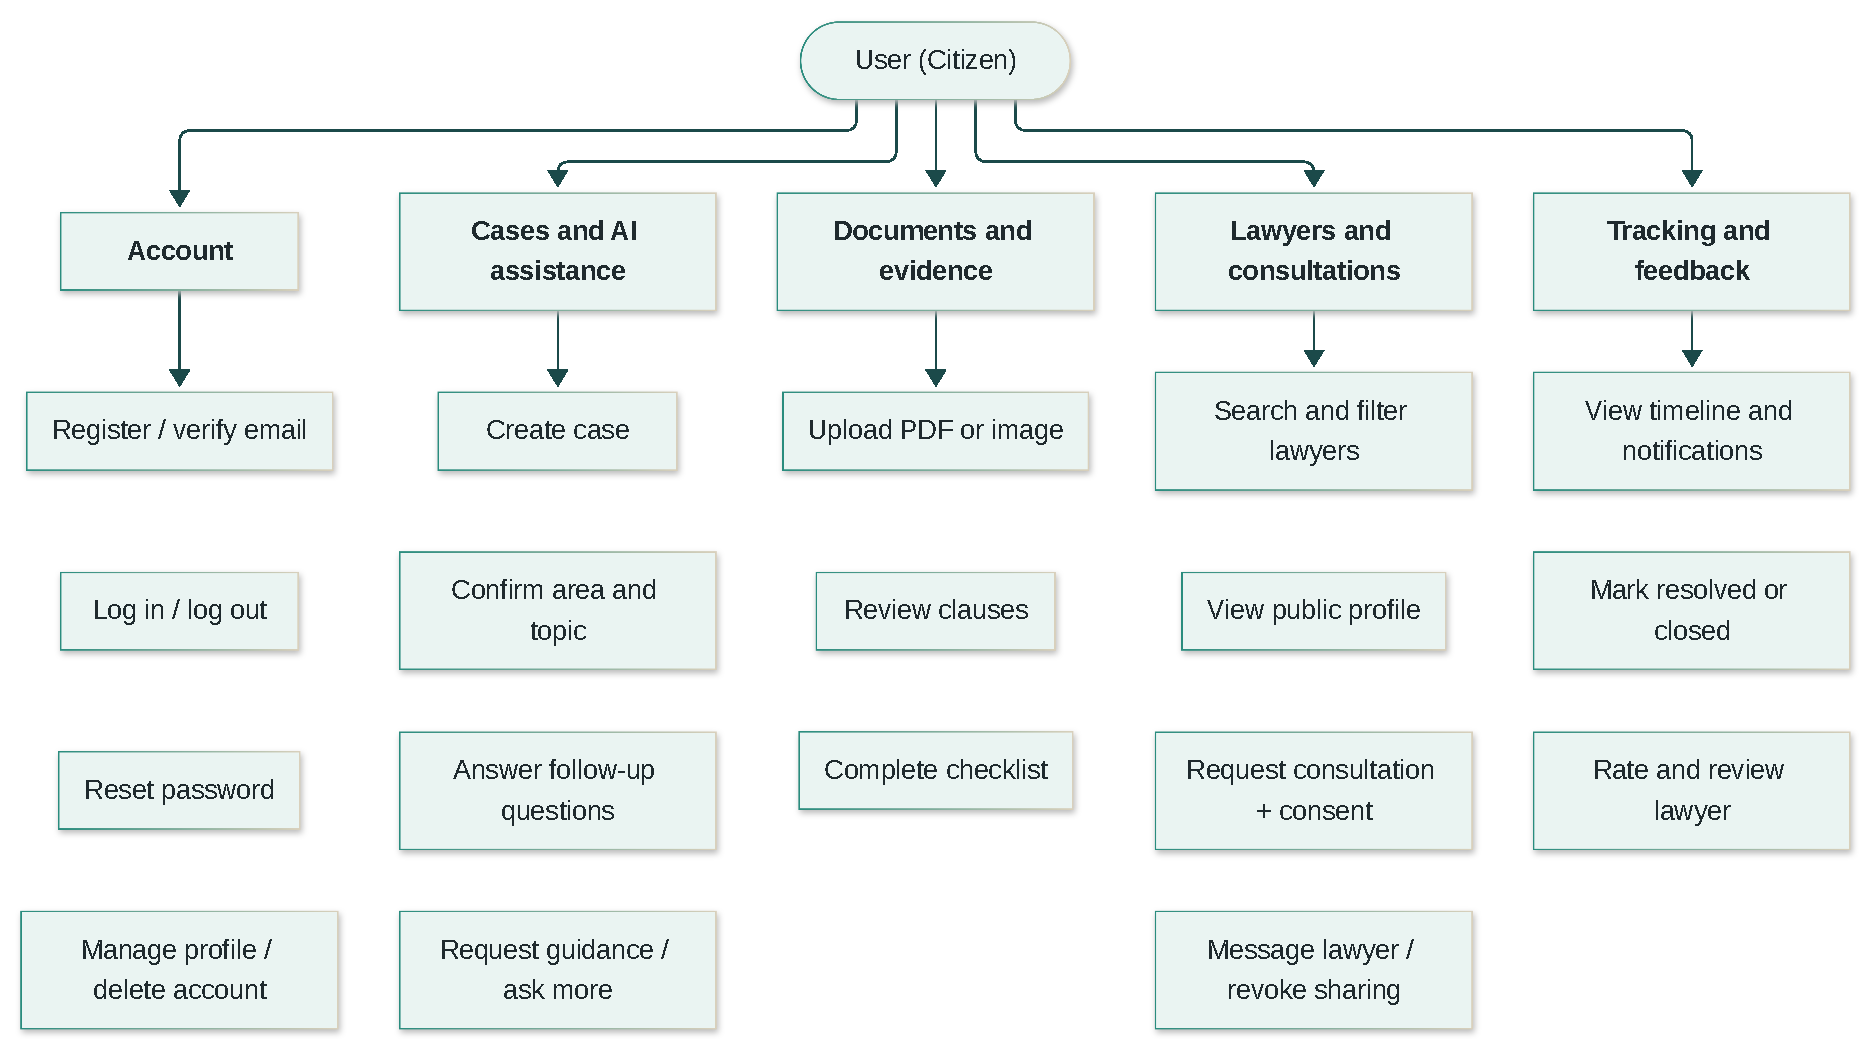
\includegraphics[width=\textwidth,height=0.80\textheight,keepaspectratio]{figures/actions_user.pdf}
\caption{Actions available to the User}\label{fig:2.1}
\end{figure}

\needspace{12\baselineskip}
\section{U-WF1: Account Access and Profile Management}

The user registers, verifies the email address and logs in. From the dashboard the user can update the profile or request account deletion. If the account has been suspended by the Admin (A-WF3), login is refused.

% Mermaid source:
% %% name: wf_u1_account
% flowchart TD
%     S(["Start"]) --> H{{"Has an account?"}}
%     H -->|No| R["Fill registration form"]
%     R --> V1{{"Email unused and input valid?"}}
%     V1 -->|No| R
%     V1 -->|Yes| E["Receive verification email"]
%     E --> C{{"Link valid?"}}
%     C -->|No| E2["Request new link"] --> E
%     C -->|Yes| ACT["Account activated"]
%     ACT --> LG
%     H -->|Yes| LG["Enter email and password"]
%     LG --> OK{{"Credentials valid?"}}
%     OK -->|No| F{{"Forgot password?"}}
%     F -->|Yes| RP["Reset via emailed link"] --> LG
%     F -->|No| LG
%     OK -->|Yes| SUS{{"Account suspended?"}}
%     SUS -->|Yes| X(["Access refused"])
%     SUS -->|No| D["User dashboard"]
%     D --> P{{"Choose action"}}
%     P -->|Edit profile| EP["Update details / password"] --> D
%     P -->|Delete account| DEL["Confirm deletion"] --> END1(["Data removed or anonymised"])
%     P -->|Continue| END2(["Go to cases (U-WF2)"])
%     ADM["Admin: A-WF3 suspension"] -.-> SUS
\begin{figure}[H]\centering
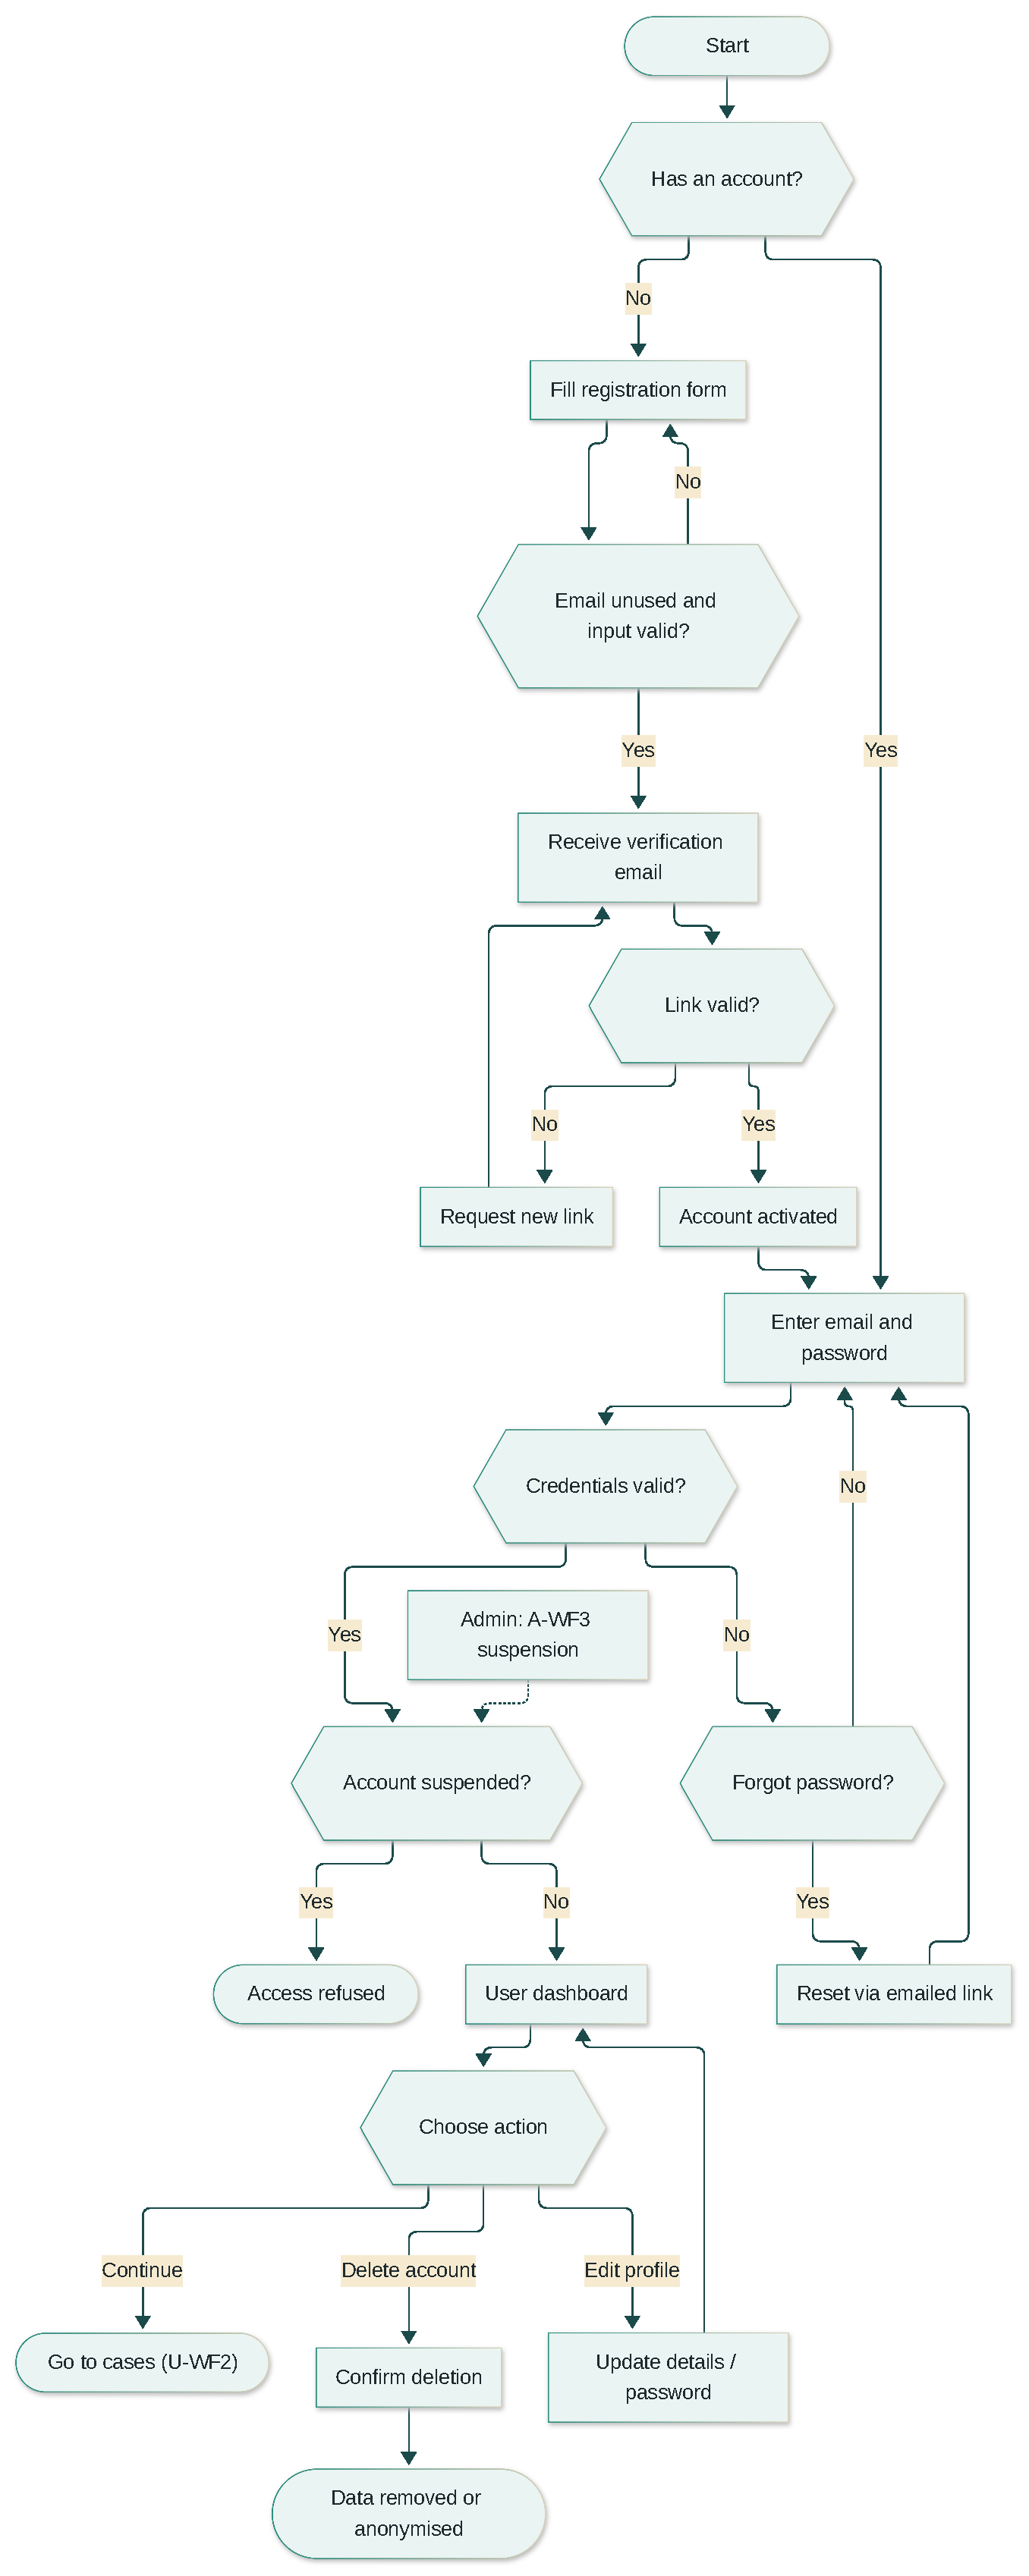
\includegraphics[width=\textwidth,height=0.80\textheight,keepaspectratio]{figures/wf_u1_account.pdf}
\caption{U-WF1 Account access and profile management}\label{fig:2.2}
\end{figure}

\needspace{12\baselineskip}
\section{U-WF2: Create Case and Clarify Facts}

The user describes the problem in free text. The system classifies the legal area and topic, and the user can correct this. The system then asks follow-up questions until all required facts for the topic are known. A question outside property and family law ends the workflow with a referral to the lawyer directory.

% Mermaid source:
% %% name: wf_u2_case
% flowchart TD
%     S(["Start: New case"]) --> D["Describe problem in own words"]
%     D --> CR["System creates case and chat session"]
%     CR --> CL["System classifies legal area and topic"]
%     CL --> SC{{"Within property or family law?"}}
%     SC -->|No| OUT["Explain scope and suggest lawyer search"] --> E0(["Go to U-WF5"])
%     SC -->|Yes| CF{{"User agrees with classification?"}}
%     CF -->|No| CH["User changes area or topic"] --> MF
%     CF -->|Yes| MF["System finds missing facts"]
%     MF --> ANY{{"Any fact missing?"}}
%     ANY -->|Yes| Q["System asks one follow-up question"]
%     Q --> A{{"User response"}}
%     A -->|Answer| ST["Store answer"] --> MF
%     A -->|Not sure| UN["Record fact as unknown"] --> MF
%     A -->|Upload document| UP["U-WF4 extracts facts"] --> MF
%     ANY -->|No| CLR["Case status: Clarified"]
%     CLR --> E(["Ready for guidance (U-WF3)"])
\begin{figure}[H]\centering
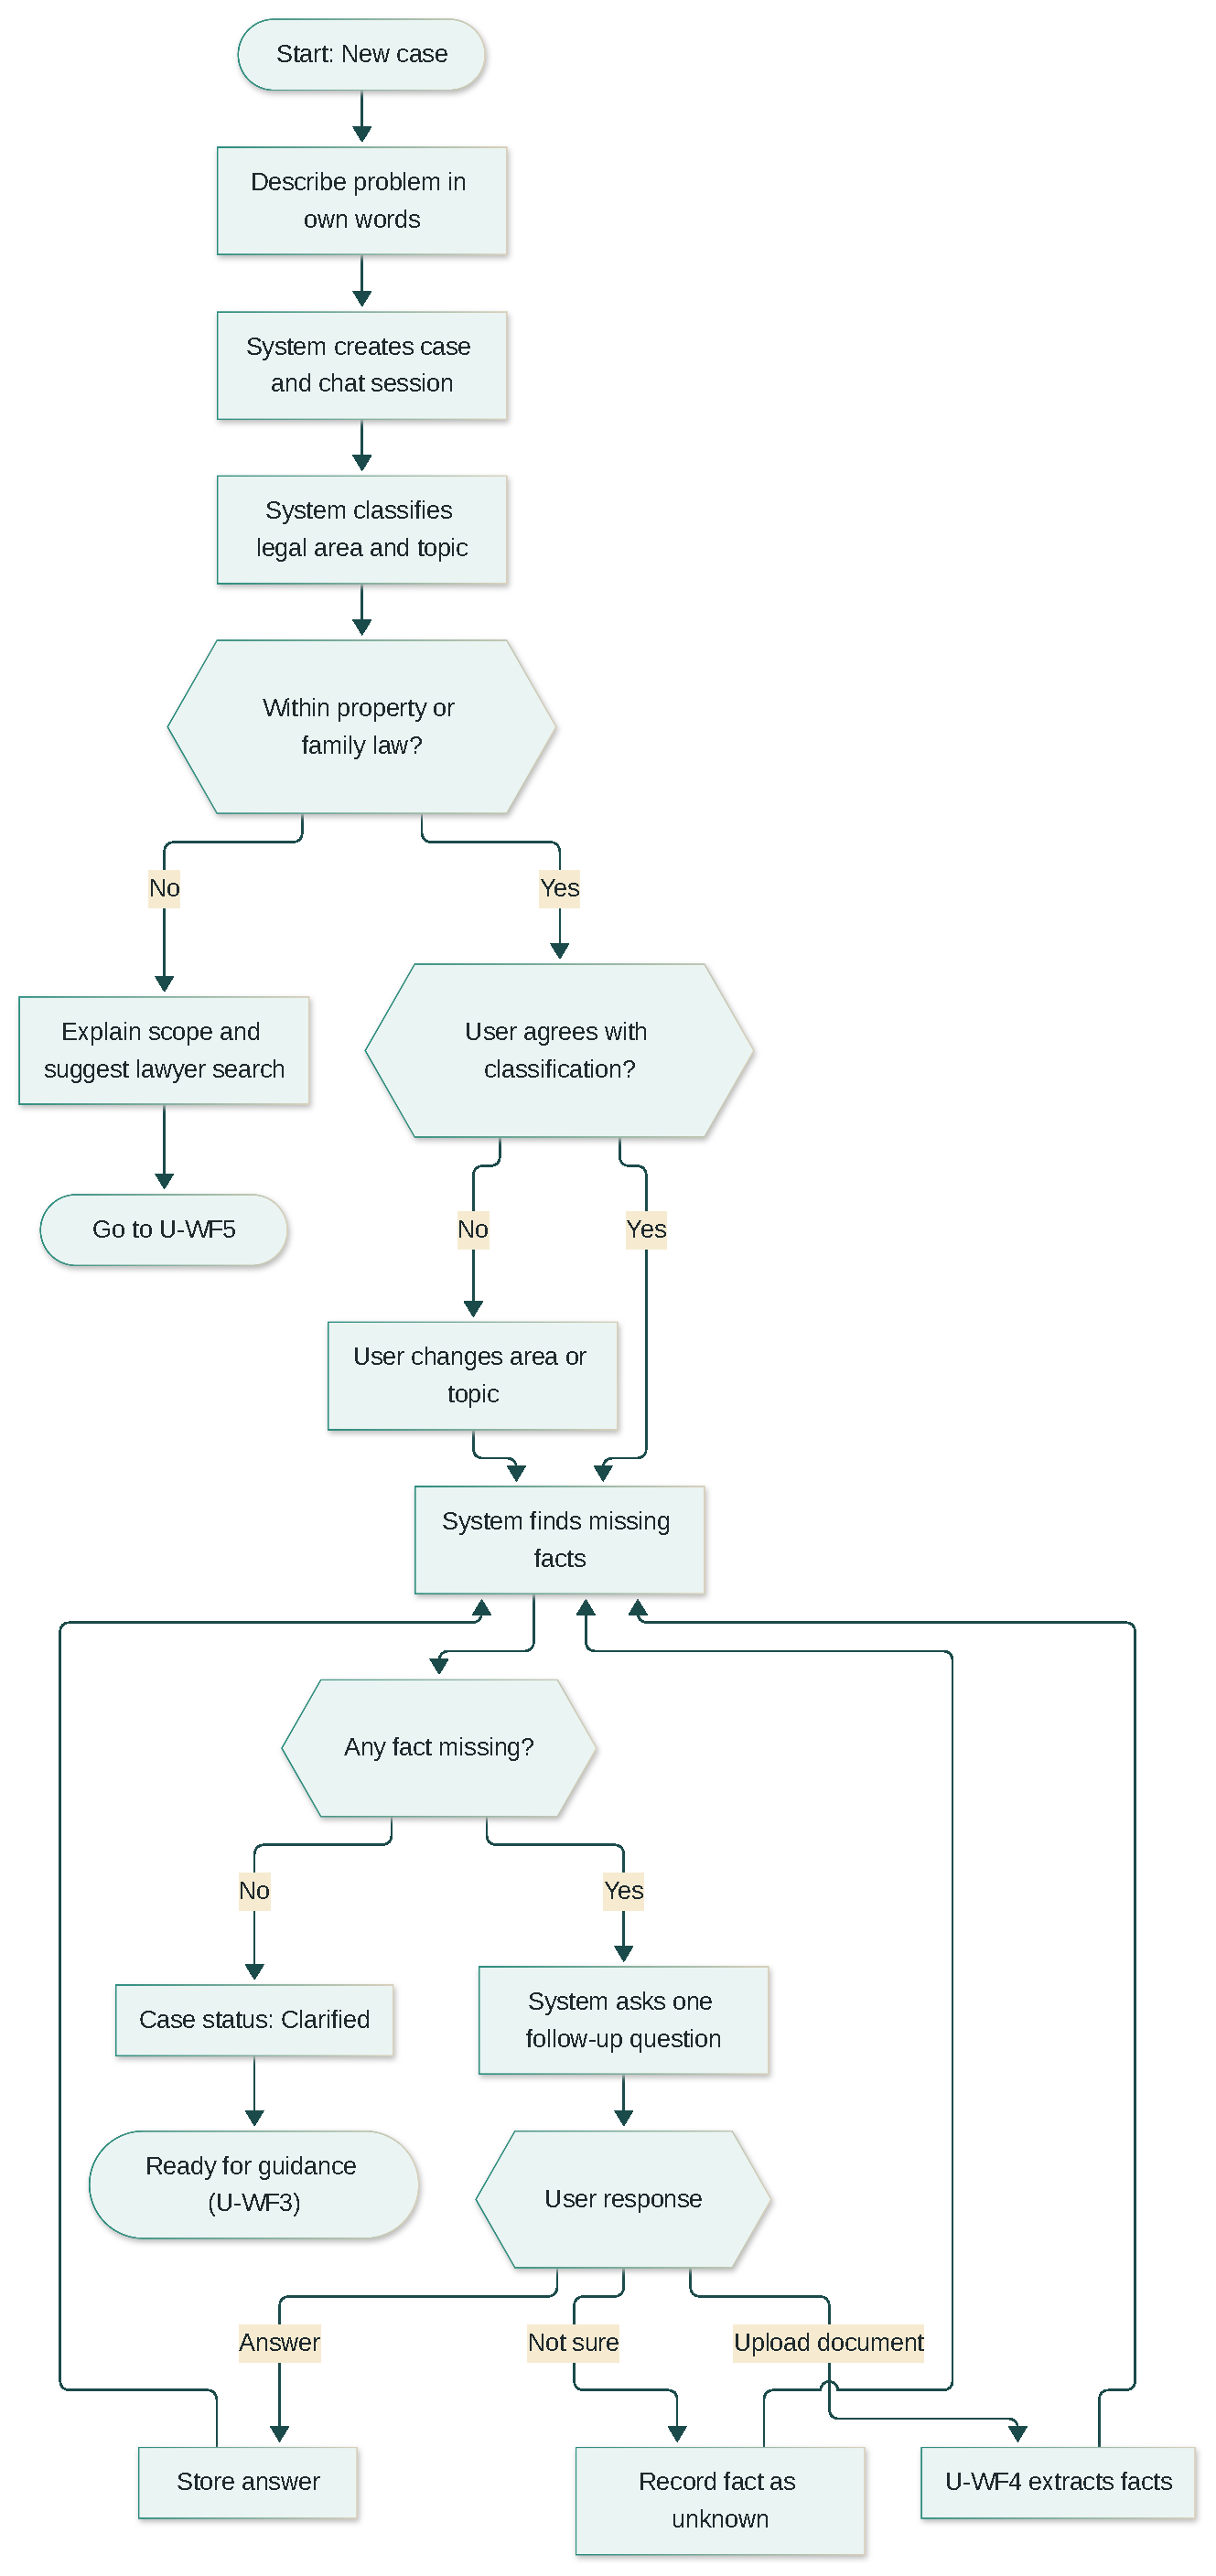
\includegraphics[width=\textwidth,height=0.80\textheight,keepaspectratio]{figures/wf_u2_case.pdf}
\caption{U-WF2 Create case and clarify facts}\label{fig:2.3}
\end{figure}

\needspace{12\baselineskip}
\section{U-WF3: Obtain AI Legal Guidance}

Guidance can be requested only for a clarified case and depends on the knowledge base prepared by the Admin (A-WF2). The automated steps are detailed in S-WF1. The user either receives a cited answer or an honest ``no verified source'' response that points to the lawyer directory.

% Mermaid source:
% %% name: wf_u3_guidance
% flowchart TD
%     S(["Start: Case is Clarified"]) --> RQ["Request guidance"]
%     RQ --> P["System runs RAG pipeline (S-WF1)"]
%     KB["Admin: verified knowledge base (A-WF2)"] -.-> P
%     P --> R{{"Result"}}
%     R -->|Cited answer| SH["Read plain-language answer, sources and disclaimer"]
%     R -->|No verified source| NS["Message: no verified source, consult a lawyer"]
%     R -->|Service error| ERR["Error shown, case kept"] --> RT{{"Retry later?"}}
%     RT -->|Yes| RQ
%     RT -->|No| E3(["End"])
%     SH --> CK["View evidence checklist"]
%     CK --> NX{{"Next step"}}
%     NX -->|Ask more| FQ["Ask follow-up question in same session"] --> P
%     NX -->|Add evidence| E1(["Go to U-WF4"])
%     NX -->|Find lawyer| E2(["Go to U-WF5"])
%     NS --> E2
\begin{figure}[H]\centering
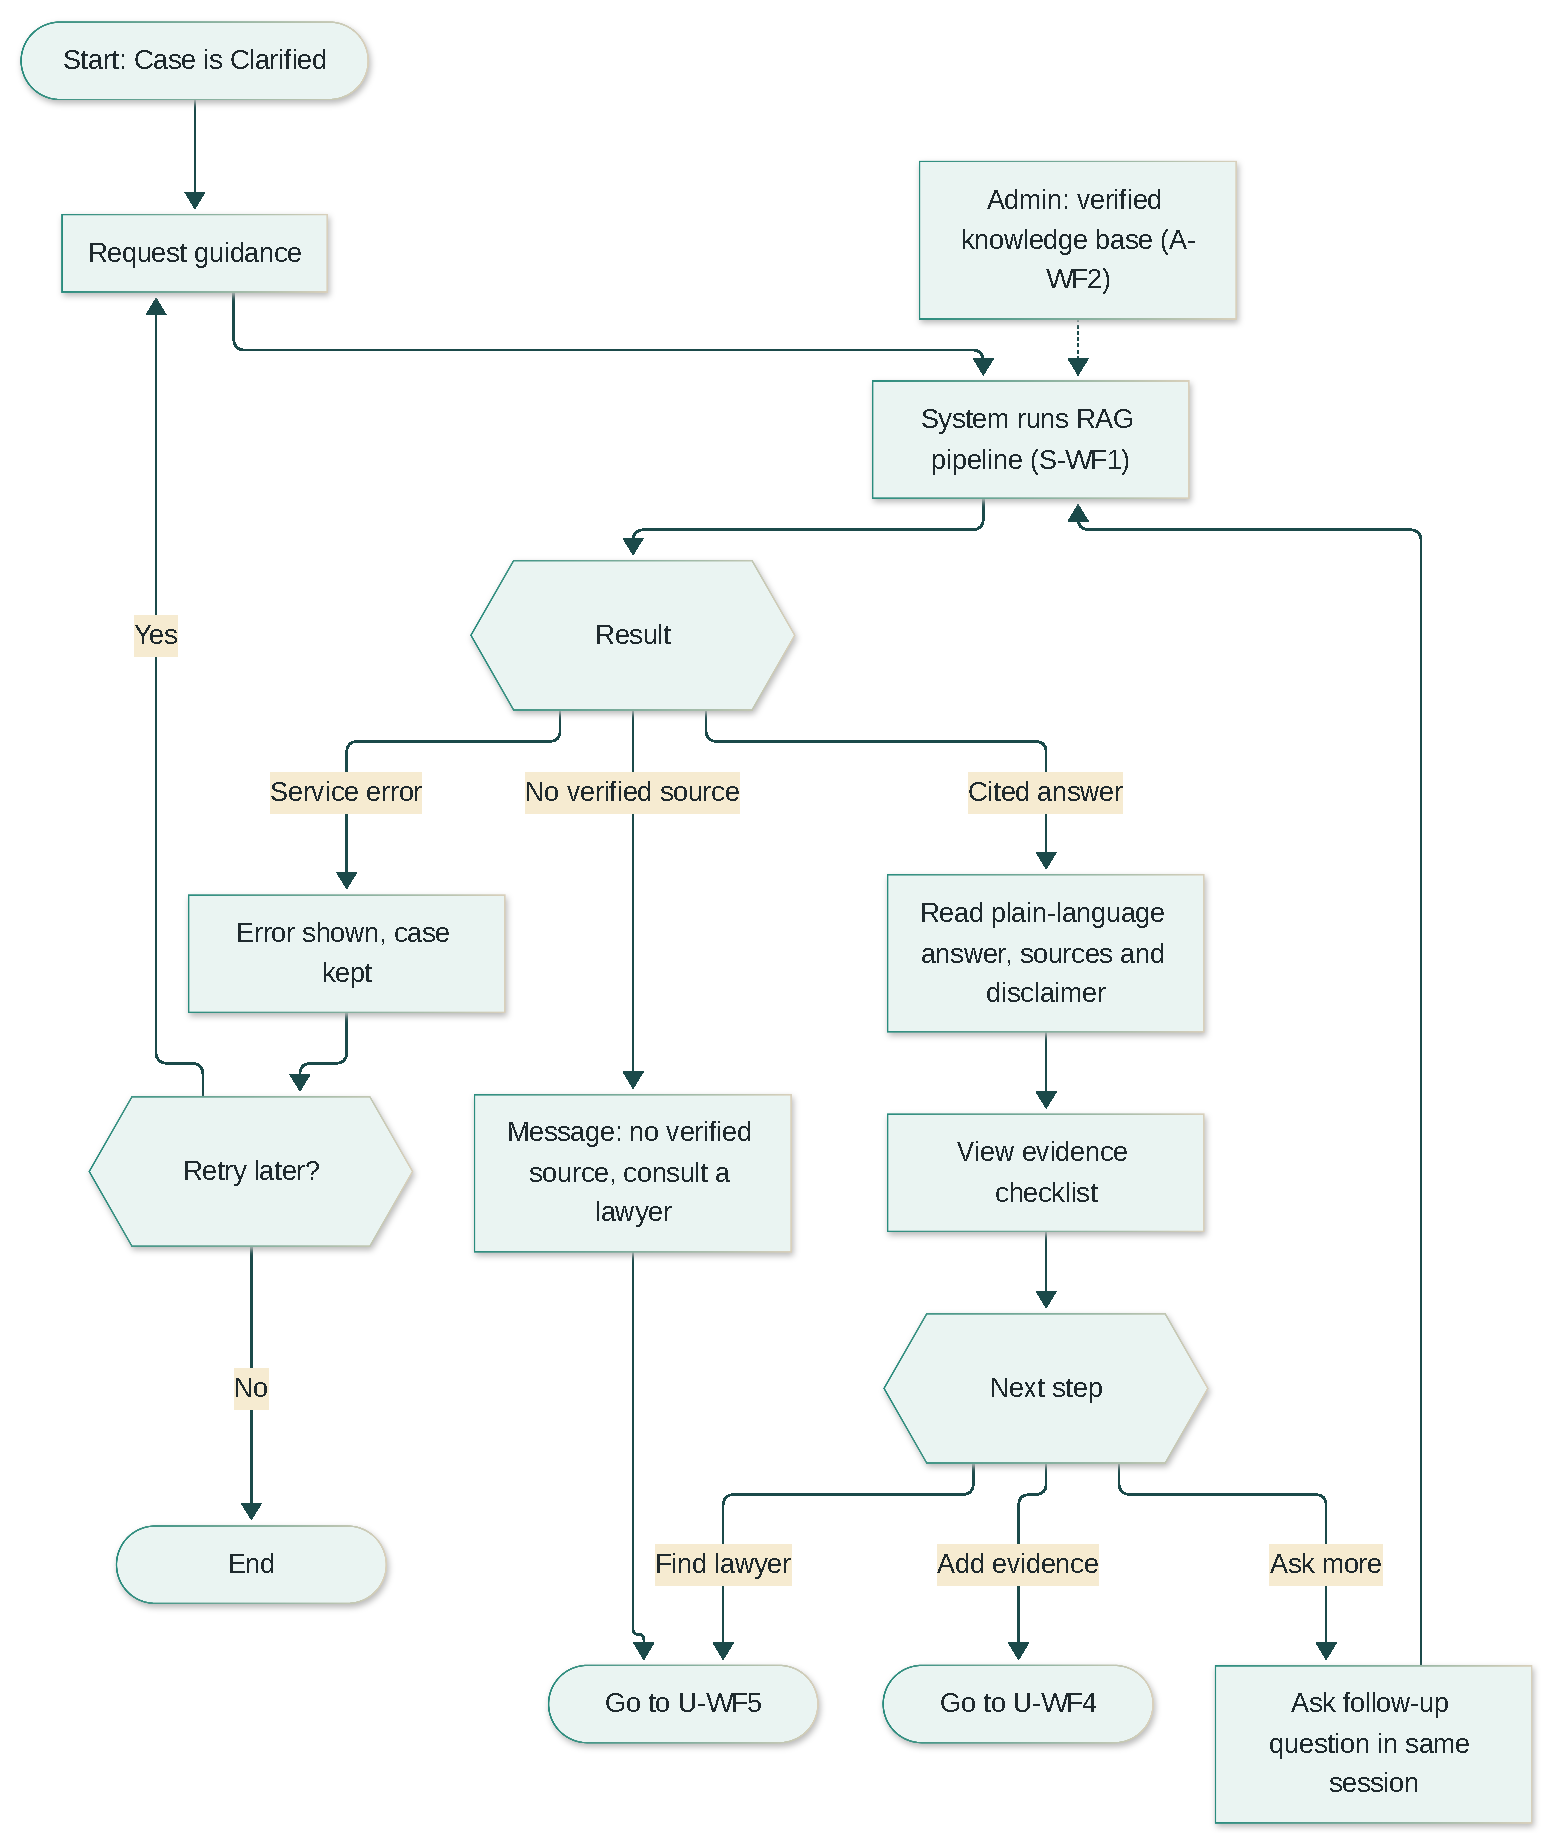
\includegraphics[width=\textwidth,height=0.80\textheight,keepaspectratio]{figures/wf_u3_guidance.pdf}
\caption{U-WF3 Obtain AI legal guidance}\label{fig:2.4}
\end{figure}

\needspace{12\baselineskip}
\section{U-WF4: Upload Documents and Complete Evidence Checklist}

Documents can be uploaded at any time after a case exists. Text extraction (PyMuPDF or OCR) and clause extraction are automated in S-WF2. Uploaded documents that match checklist items mark those items as available.

% Mermaid source:
% %% name: wf_u4_documents
% flowchart TD
%     S(["Start: Case exists"]) --> SEL["Select case and file"]
%     SEL --> VAL{{"Type PDF/JPG/PNG and size within limit?"}}
%     VAL -->|No| REJ["Upload rejected with reason"] --> SEL
%     VAL -->|Yes| UPL["File uploaded"]
%     UPL --> PROC["System processes document (S-WF2)"]
%     PROC --> Q{{"Text readable?"}}
%     Q -->|No| LOWQ["Asked for clearer image, file marked low quality"] --> SEL
%     Q -->|Yes| CLS["Review extracted key clauses"]
%     CLS --> LBL{{"Clauses recognised?"}}
%     LBL -->|No| MAN["Label document type manually"] --> CHK
%     LBL -->|Yes| CHK["Checklist items updated"]
%     CHK --> DONE{{"All required items available?"}}
%     DONE -->|No| MORE["Upload next document"] --> SEL
%     DONE -->|Yes| E(["Evidence complete"])
\begin{figure}[H]\centering
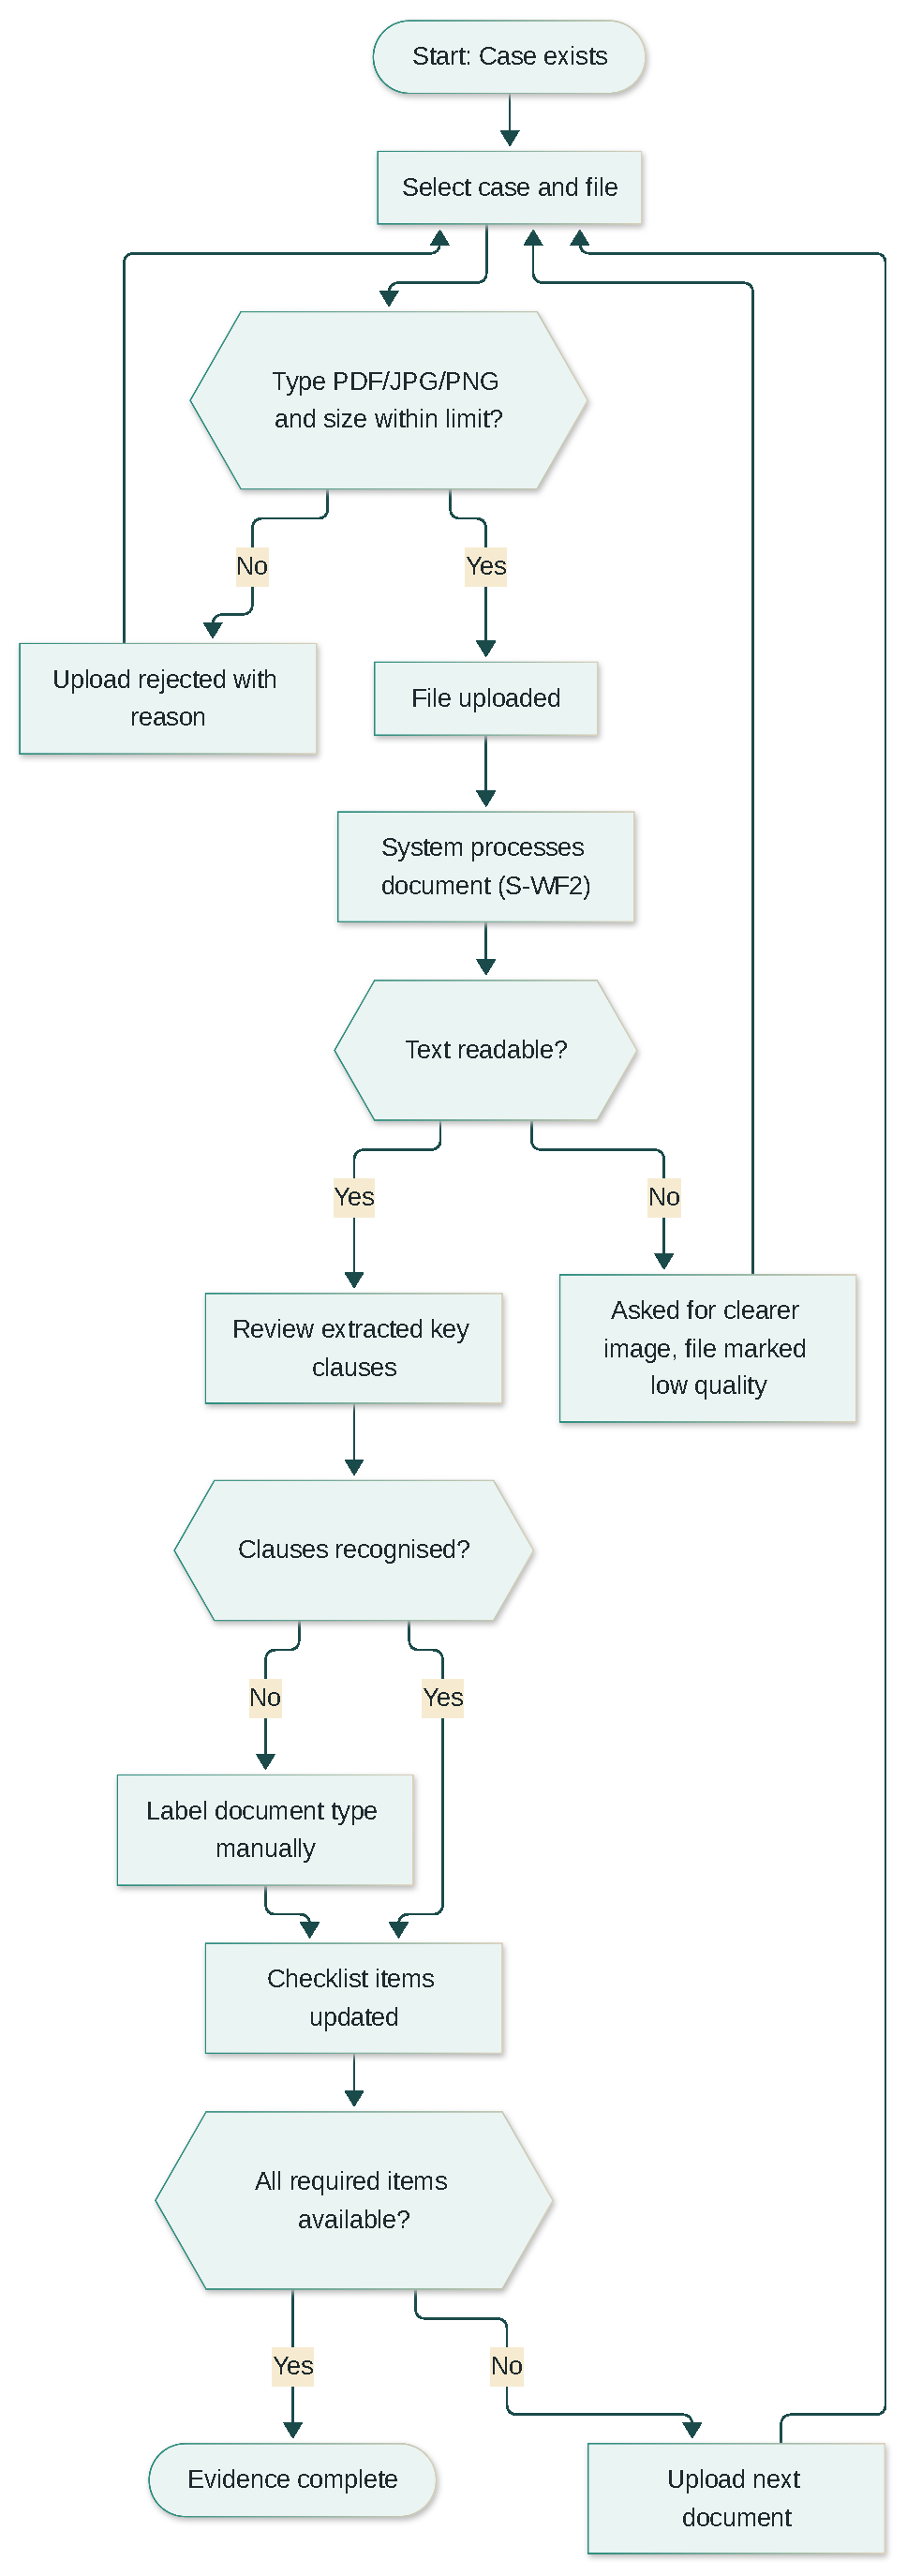
\includegraphics[width=\textwidth,height=0.80\textheight,keepaspectratio]{figures/wf_u4_documents.pdf}
\caption{U-WF4 Upload documents and complete evidence checklist}\label{fig:2.5}
\end{figure}

\needspace{12\baselineskip}
\section{U-WF5: Find a Lawyer and Request a Consultation}

The directory shows only lawyers verified by the Admin (A-WF1) whose profiles are published (L-WF2). A consultation is created only after explicit consent, and the request is delivered to the lawyer, who handles it in L-WF3.

% Mermaid source:
% %% name: wf_u5_consult
% flowchart TD
%     S(["Start"]) --> DIR["Open lawyer directory"]
%     VER["Admin: lawyers verified (A-WF1)"] -.-> DIR
%     DIR --> FIL["Apply filters: area, city, fee, experience, language, rating"]
%     FIL --> RES{{"Matches found?"}}
%     RES -->|No| WID["Widen filters"] --> FIL
%     RES -->|Yes| PRO["Open public profile"]
%     PRO --> FIT{{"Suitable lawyer?"}}
%     FIT -->|No| FIL
%     FIT -->|Yes| AV{{"Lawyer accepting requests?"}}
%     AV -->|No| FIL
%     AV -->|Yes| REQ["Choose case, mode, time and message"]
%     REQ --> CON["Review items to be shared"]
%     CON --> AG{{"Give consent?"}}
%     AG -->|No| C0(["No consultation created"])
%     AG -->|Yes| CR["Consultation Requested, consent recorded"]
%     CR --> NT["Lawyer notified (S-WF4)"]
%     NT --> E(["Await lawyer response (L-WF3)"])
\begin{figure}[H]\centering
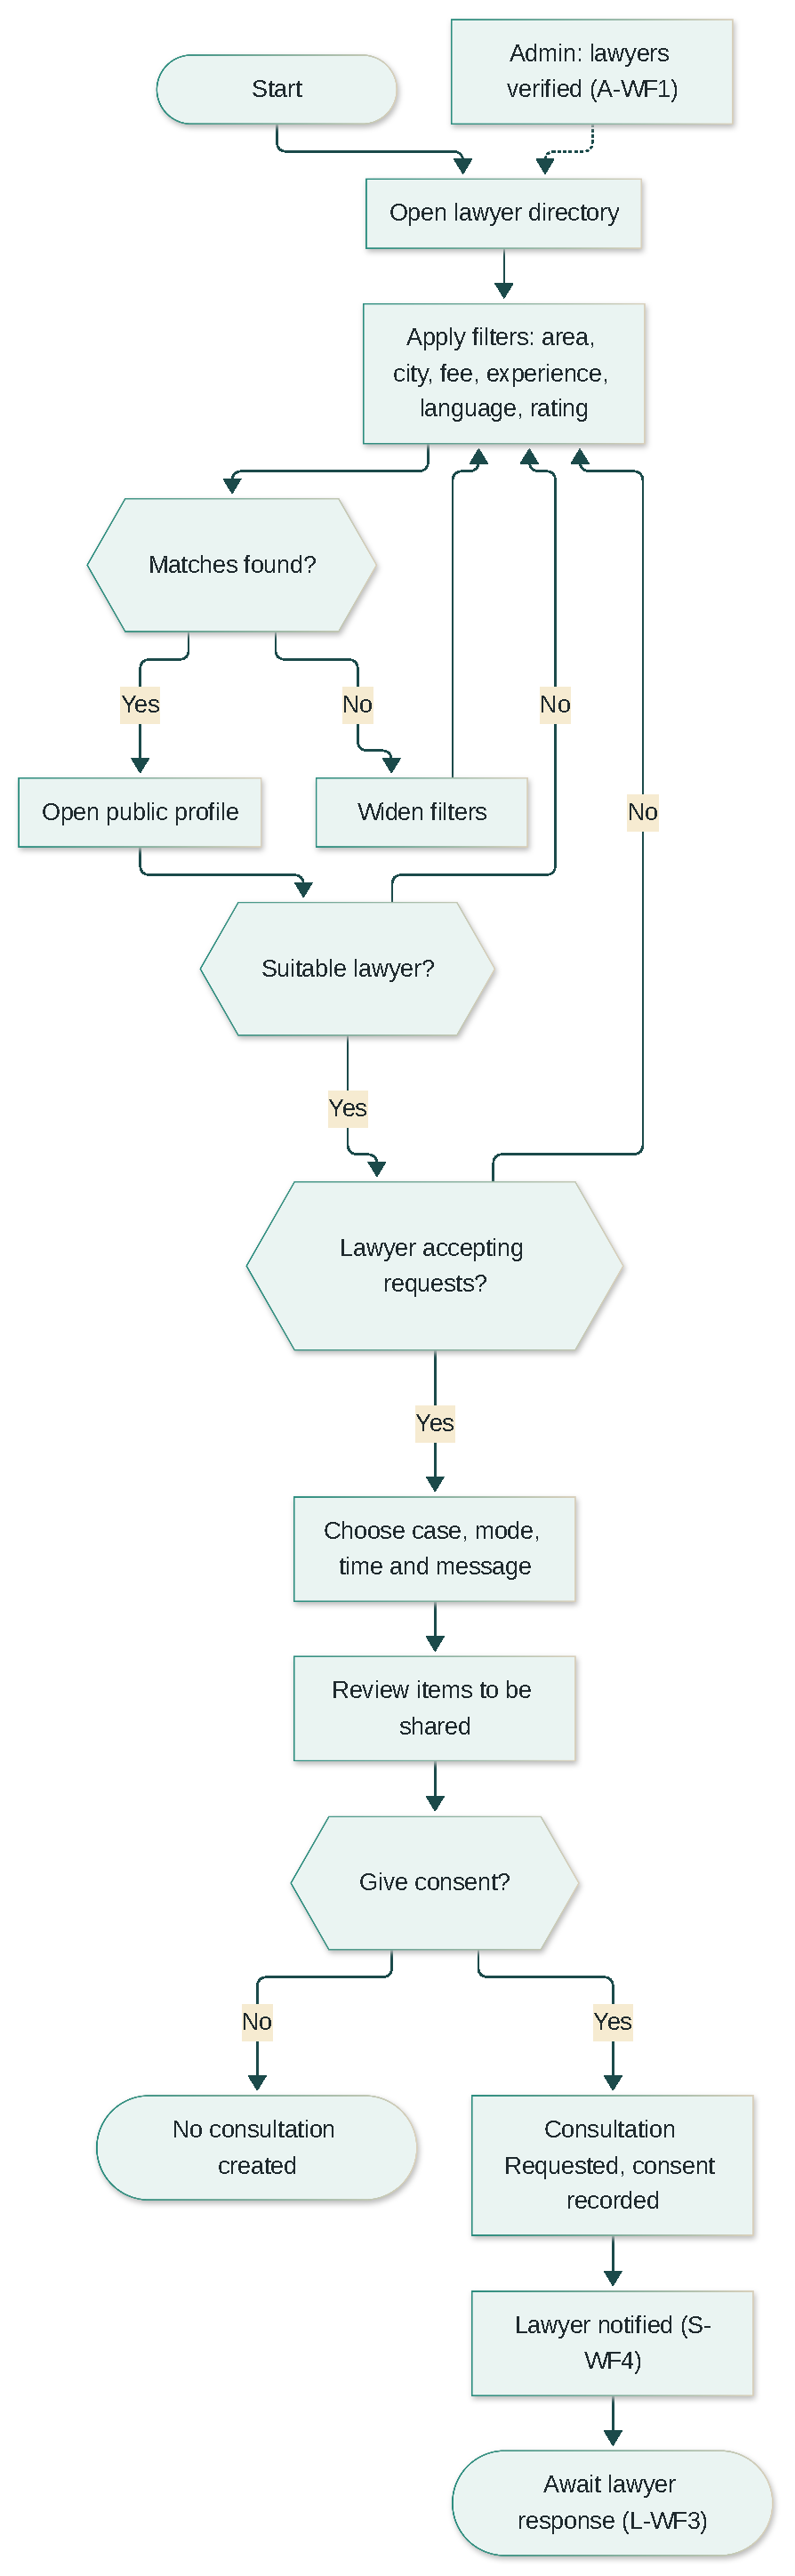
\includegraphics[width=\textwidth,height=0.80\textheight,keepaspectratio]{figures/wf_u5_consult.pdf}
\caption{U-WF5 Find a lawyer and request a consultation}\label{fig:2.6}
\end{figure}

\needspace{12\baselineskip}
\section{U-WF6: Track Case, Communicate and Review}

The user follows the case timeline, receives notifications of lawyer actions, can message the lawyer within an accepted consultation, can revoke sharing at any time, and reviews the lawyer after the consultation is completed.

% Mermaid source:
% %% name: wf_u6_track
% flowchart TD
%     S(["Start: Open case"]) --> TL["View status, timeline, checklist and consultations"]
%     TL --> EV{{"Event or user choice"}}
%     EV -->|Lawyer update received| UPD["Read update (from L-WF4)"] --> TL
%     EV -->|Consultation accepted| MSG["Message lawyer"] --> TL
%     EV -->|Stop sharing| REV["Revoke consent"] --> RV2["Lawyer access ends, timeline records revocation"] --> TL
%     EV -->|Consultation completed| RW{{"Leave a review?"}}
%     RW -->|Yes| RATE["Rate 1-5 and comment"] --> TL
%     RW -->|No| TL
%     EV -->|Matter settled| RES["Mark case Resolved"] --> E1(["End"])
%     EV -->|Abandon| CLS["Close case"] --> E2(["End"])
\begin{figure}[H]\centering
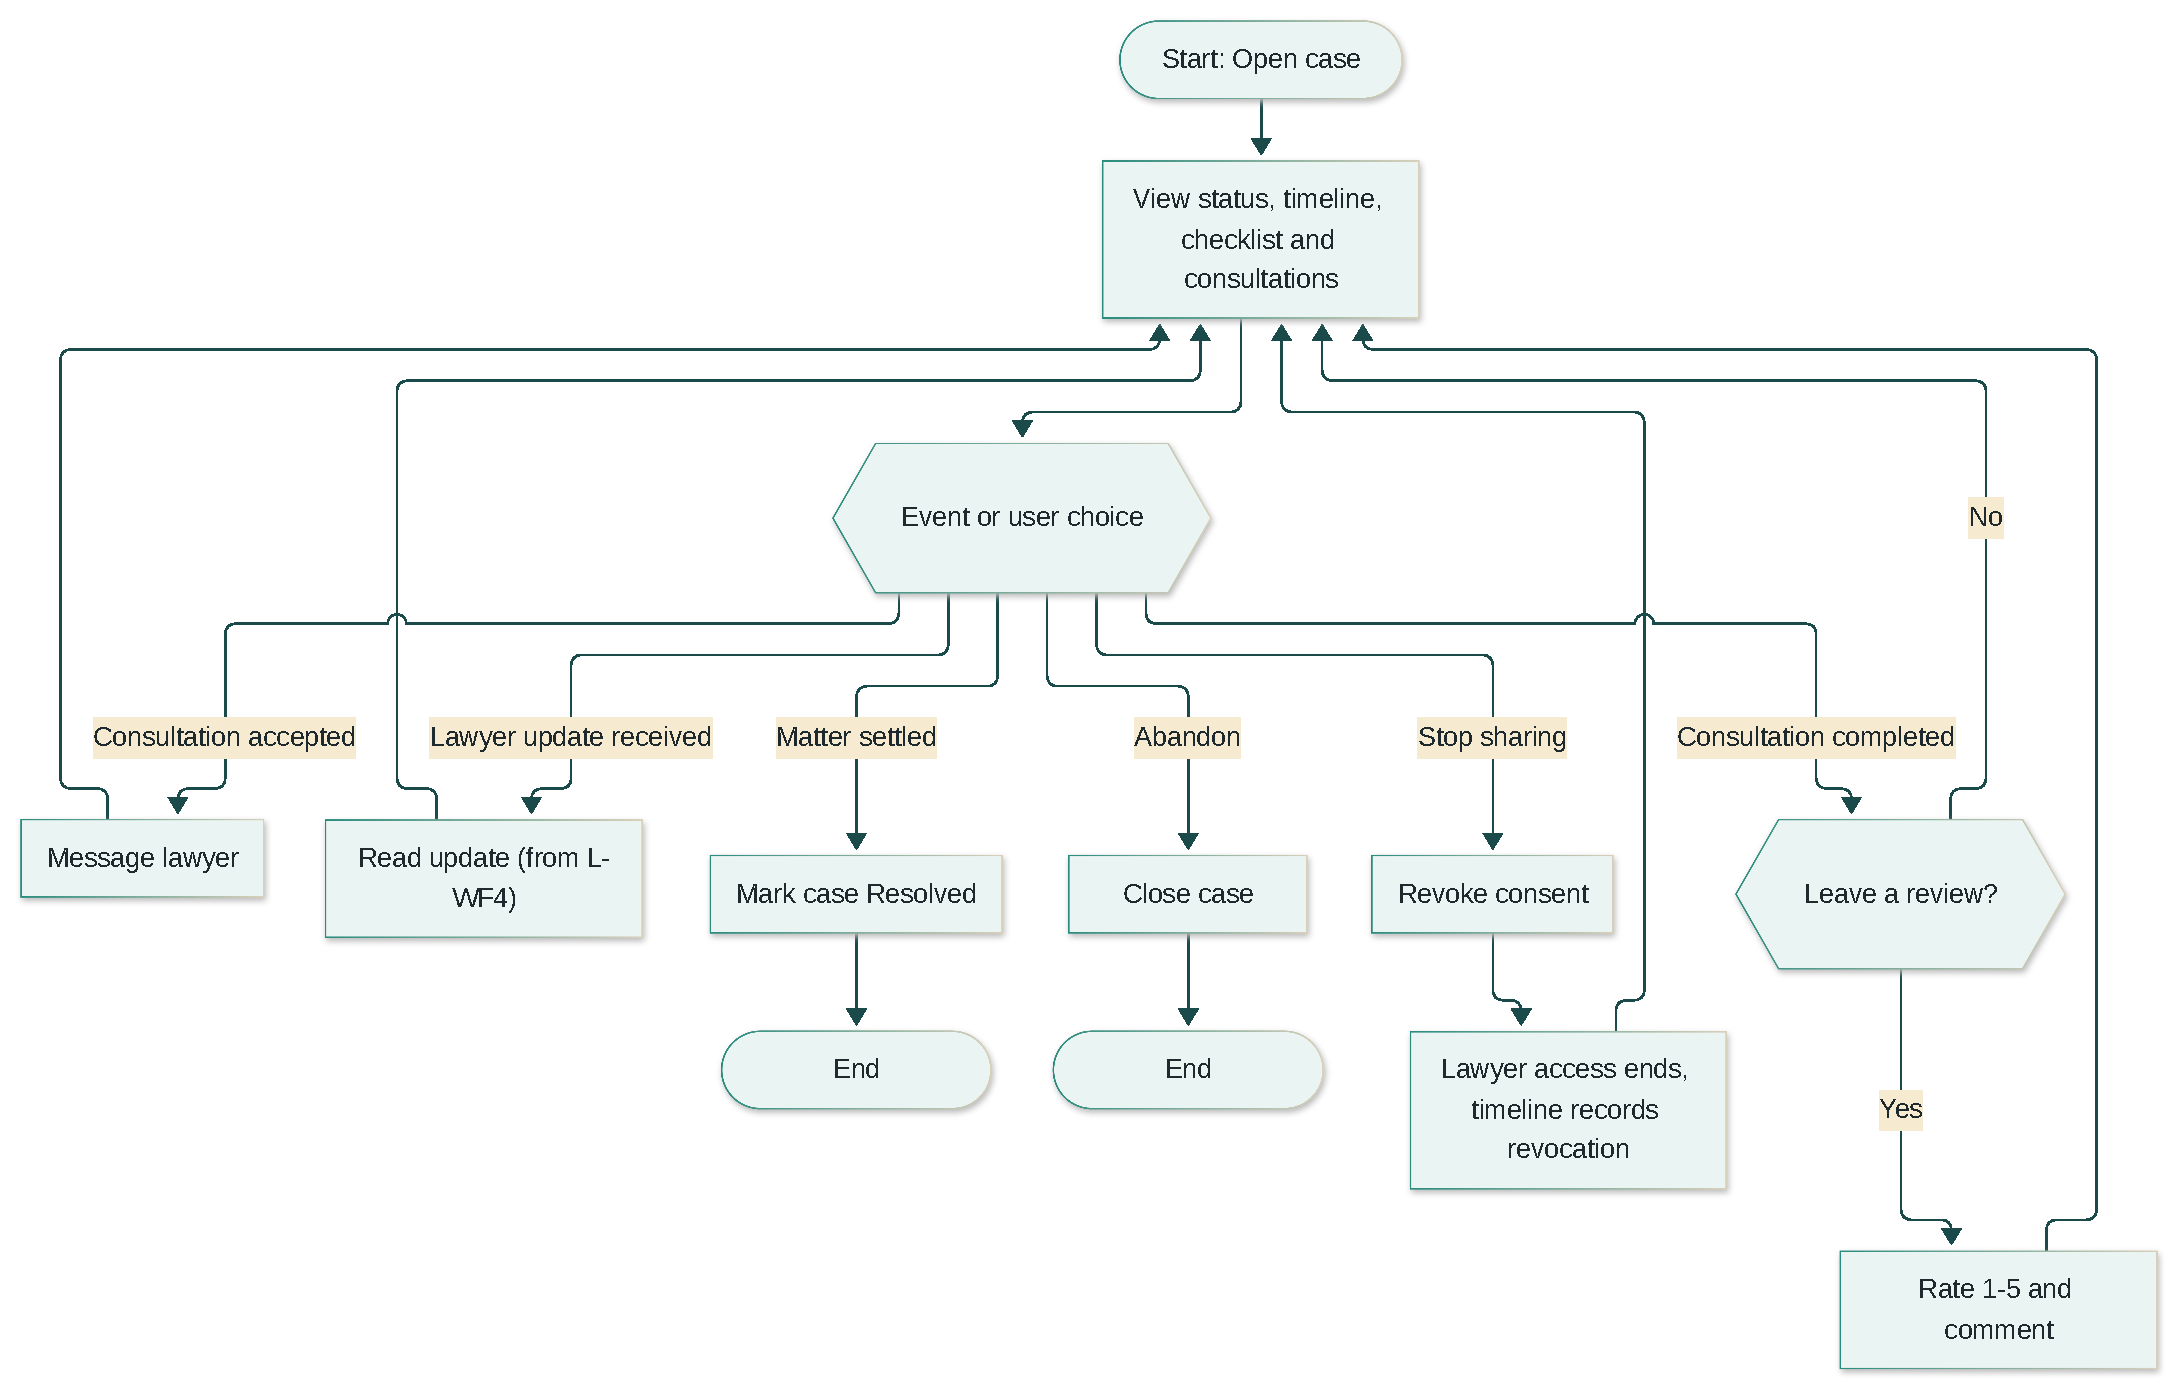
\includegraphics[width=\textwidth,height=0.80\textheight,keepaspectratio]{figures/wf_u6_track.pdf}
\caption{U-WF6 Track case, communicate and review}\label{fig:2.7}
\end{figure}

\chapter{Lawyer Workflows}\label{ch:3}

\section{Lawyer Actions and Dependencies}

\begin{longtable}{|L{1.87cm}|L{4.05cm}|L{2.81cm}|L{3.12cm}|L{1.70cm}|}
\caption{Actions of the Lawyer and their dependencies}\label{tab:3.1}\\
\hline\headrow \thd{ID} & \thd{Action} & \thd{Depends on} & \thd{Result} & \thd{Req.} \\ \hline
\endfirsthead
\hline\headrow \thd{ID} & \thd{Action} & \thd{Depends on} & \thd{Result} & \thd{Req.} \\ \hline
\endhead
\hline\endlastfoot
L-A01 & Register as lawyer with bar details and licence & Valid email & Account pending verification & LFR-01 \\ \hline
L-A02 & Log in / log out & Verified email; not suspended (A-WF3) & Lawyer dashboard & LFR-02 \\ \hline
L-A03 & Build or edit public profile & L-A02 & Profile saved (preview) & LFR-03 \\ \hline
L-A04 & Submit or re-submit verification request & L-A01 & Request in Admin queue & LFR-01 \\ \hline
L-A05 & Profile published in directory & Admin approval (A-WF1) & Verified badge, listed & LFR-04 \\ \hline
L-A06 & Set availability / pause requests & L-A05 & Accepting or paused & LFR-05 \\ \hline
L-A07 & View consultation requests & L-A05; user request with consent (U-WF5) & Request list & LFR-06 \\ \hline
L-A08 & Accept, decline or propose another time & L-A07 & Consultation Scheduled, Declined or Rescheduling & LFR-07 \\ \hline
L-A09 & Access shared case & Active consent (U-A16, not revoked) & Read-only case view & LFR-08 \\ \hline
L-A10 & Message user & Consultation accepted & Message thread & LFR-09 \\ \hline
L-A11 & Post case status update & Consultation accepted; active consent & Timeline entry, user notified & LFR-10 \\ \hline
L-A12 & Mark consultation completed & Consultation Scheduled & Review enabled for user & LFR-11 \\ \hline
L-A13 & View dashboard and rating & L-A02 & Statistics & LFR-12 \\
\end{longtable}

% Mermaid source:
% %% name: actions_lawyer
% flowchart TB
%     ROOT(["Lawyer"])
%     G1["<b>Account and verification</b>"]
%     ROOT --> G1
%     G1A1["Register with bar details"]
%     G1 --> G1A1
%     G1A2["Log in / log out"]
%     G1A1 ~~~ G1A2
%     G1A3["Submit or re-submit verification"]
%     G1A2 ~~~ G1A3
%     G2["<b>Public profile</b>"]
%     ROOT --> G2
%     G2A1["Edit headline, about, practice areas"]
%     G2 --> G2A1
%     G2A2["Add experience and education"]
%     G2A1 ~~~ G2A2
%     G2A3["Set fees, languages, availability"]
%     G2A2 ~~~ G2A3
%     G3["<b>Consultation requests</b>"]
%     ROOT --> G3
%     G3A1["View requests and shared summary"]
%     G3 --> G3A1
%     G3A2["Accept / decline / propose time"]
%     G3A1 ~~~ G3A2
%     G4["<b>Shared case work</b>"]
%     ROOT --> G4
%     G4A1["Read consented case items"]
%     G4 --> G4A1
%     G4A2["Message user"]
%     G4A1 ~~~ G4A2
%     G4A3["Post status updates"]
%     G4A2 ~~~ G4A3
%     G4A4["Mark consultation completed"]
%     G4A3 ~~~ G4A4
%     G5["<b>Dashboard</b>"]
%     ROOT --> G5
%     G5A1["View requests, active cases, rating"]
%     G5 --> G5A1
\begin{figure}[H]\centering
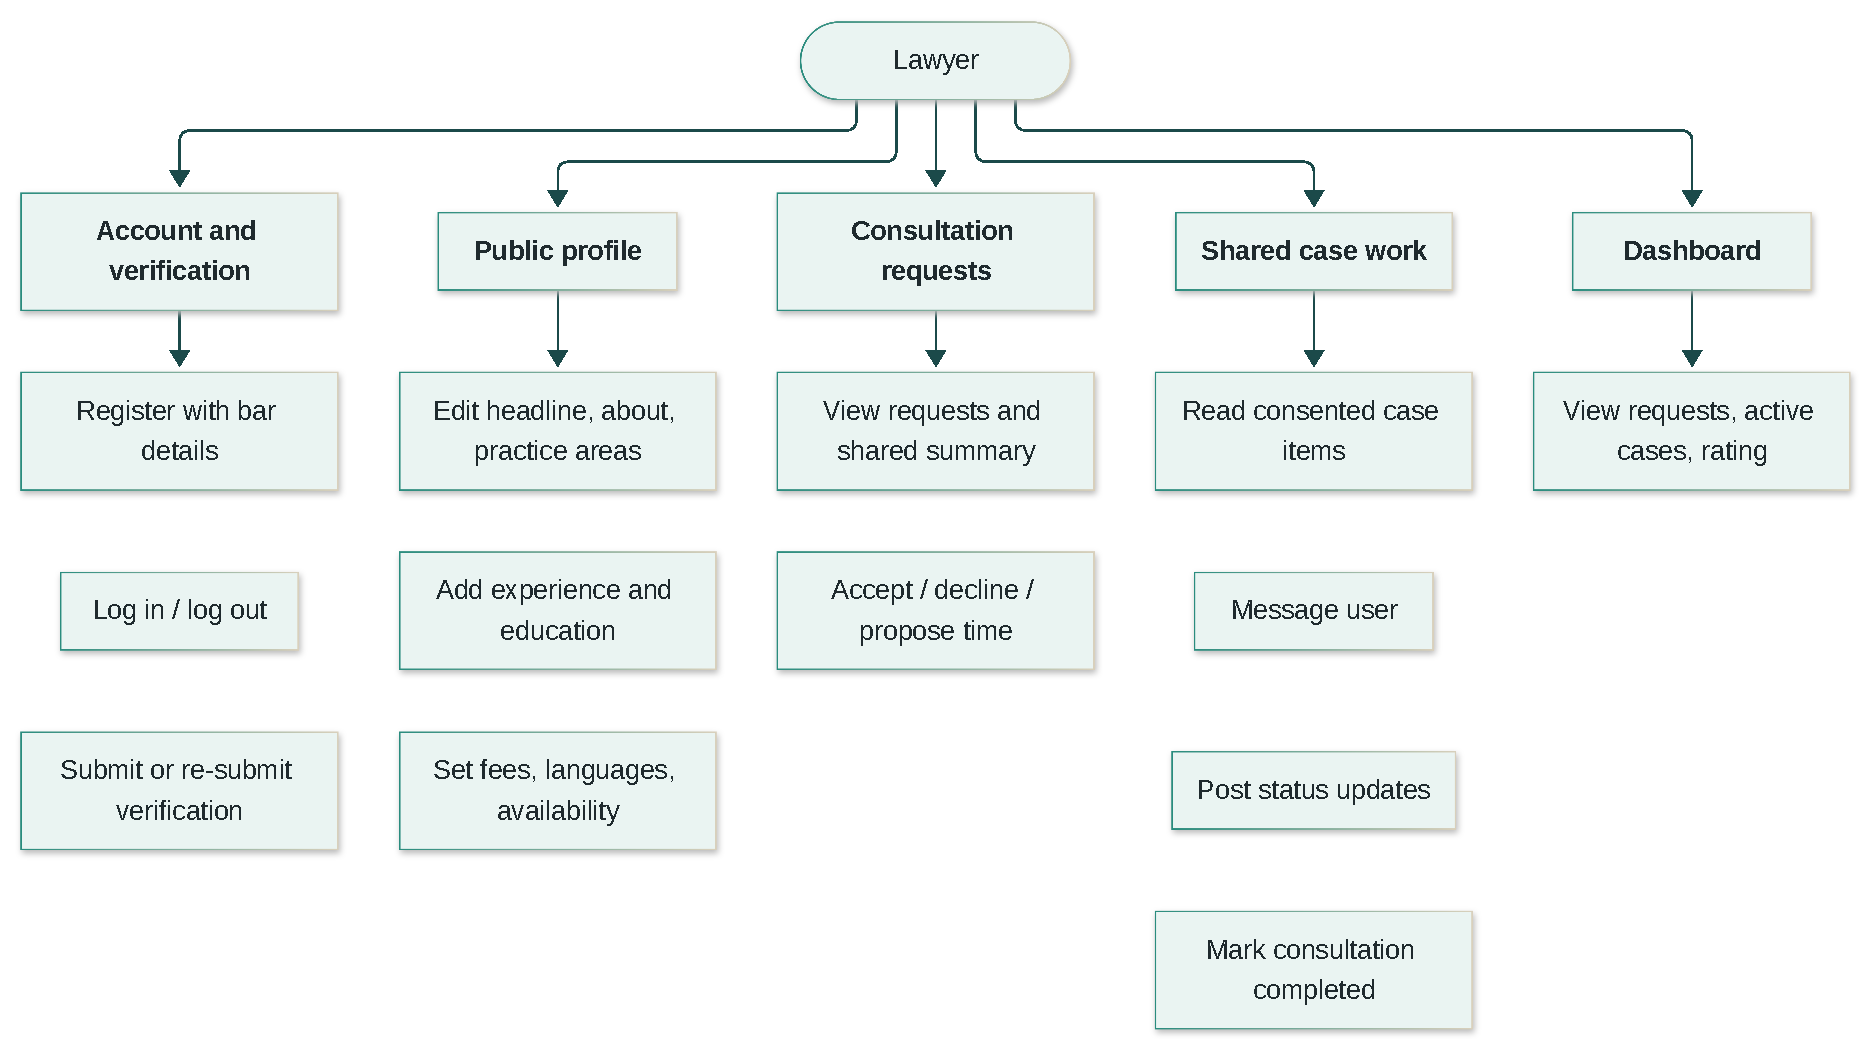
\includegraphics[width=\textwidth,height=0.80\textheight,keepaspectratio]{figures/actions_lawyer.pdf}
\caption{Actions available to the Lawyer}\label{fig:3.1}
\end{figure}

\needspace{12\baselineskip}
\section{L-WF1: Registration and Verification}

A lawyer can log in after email verification but is not listed in the directory until the Admin approves the submitted credentials (A-WF1). A rejected lawyer can correct the details and re-submit.

% Mermaid source:
% %% name: wf_l1_verify
% flowchart TD
%     S(["Start"]) --> REG["Register: personal details, bar enrolment no., bar council"]
%     REG --> LIC["Upload licence copy"]
%     LIC --> EM["Verify email"]
%     EM --> PEND["Status: Pending verification"]
%     PEND --> SUB["Verification request sent to Admin queue"]
%     SUB -.->|"handled in A-WF1"| DEC{{"Admin decision"}}
%     DEC -->|Approved| VER["Status: Verified, profile listed with badge"]
%     DEC -->|More info needed| INF["Provide clarification"] --> SUB
%     DEC -->|Rejected| REJ["Read rejection reason"]
%     REJ --> FIX{{"Correct and re-submit?"}}
%     FIX -->|Yes| CORR["Update details or licence"] --> SUB
%     FIX -->|No| E0(["Remains unlisted"])
%     VER --> E(["Can receive consultation requests"])
\begin{figure}[H]\centering
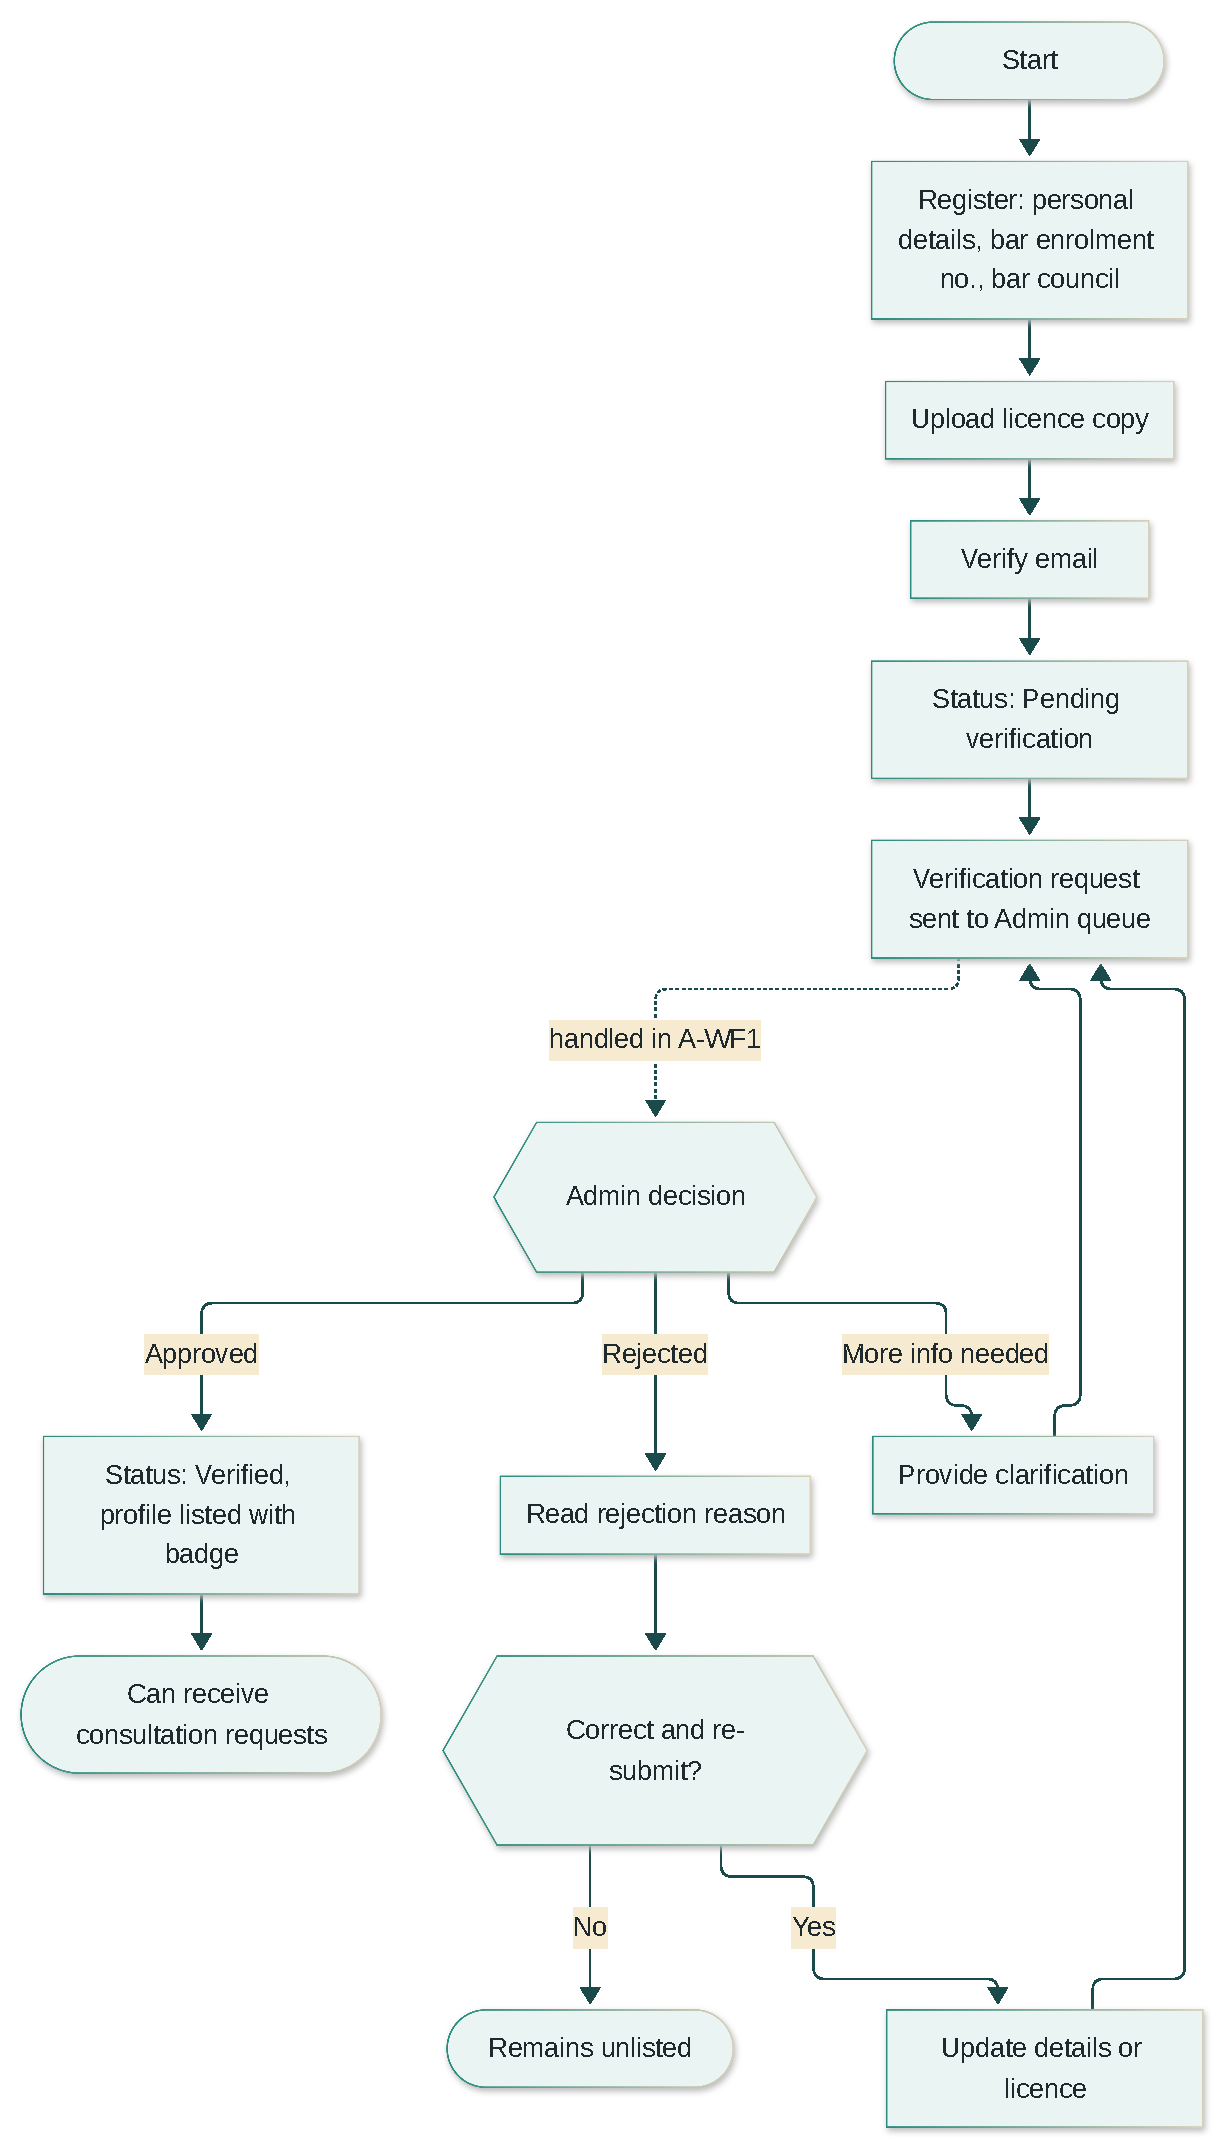
\includegraphics[width=\textwidth,height=0.80\textheight,keepaspectratio]{figures/wf_l1_verify.pdf}
\caption{L-WF1 Registration and verification}\label{fig:3.2}
\end{figure}

\needspace{12\baselineskip}
\section{L-WF2: Public Profile and Availability Management}

The profile is a LinkedIn-style public page. Edits to ordinary profile fields are published immediately for a verified lawyer. Edits to bar enrolment details return the profile to pending verification.

% Mermaid source:
% %% name: wf_l2_profile
% flowchart TD
%     S(["Start: Open My Profile"]) --> ED["Edit headline, about, practice areas, experience, education, languages, fees, photo"]
%     ED --> VAL{{"Input valid?"}}
%     VAL -->|No| ED
%     VAL -->|Yes| PRV["Preview public page"]
%     PRV --> BAR{{"Bar details changed?"}}
%     BAR -->|Yes| PEN["Status returns to Pending verification (A-WF1)"] --> E1(["Unlisted until re-approved"])
%     BAR -->|No| PUB{{"Lawyer verified?"}}
%     PUB -->|No| SAVE["Saved, not yet public"] --> E2(["Await verification"])
%     PUB -->|Yes| LIVE["Changes published in directory"]
%     LIVE --> AVL{{"Accepting new requests?"}}
%     AVL -->|Yes| ON["Availability: open"] --> E3(["Visible to users (U-WF5)"])
%     AVL -->|No| OFF["Availability: paused"] --> E4(["Listed but new requests blocked"])
\begin{figure}[H]\centering
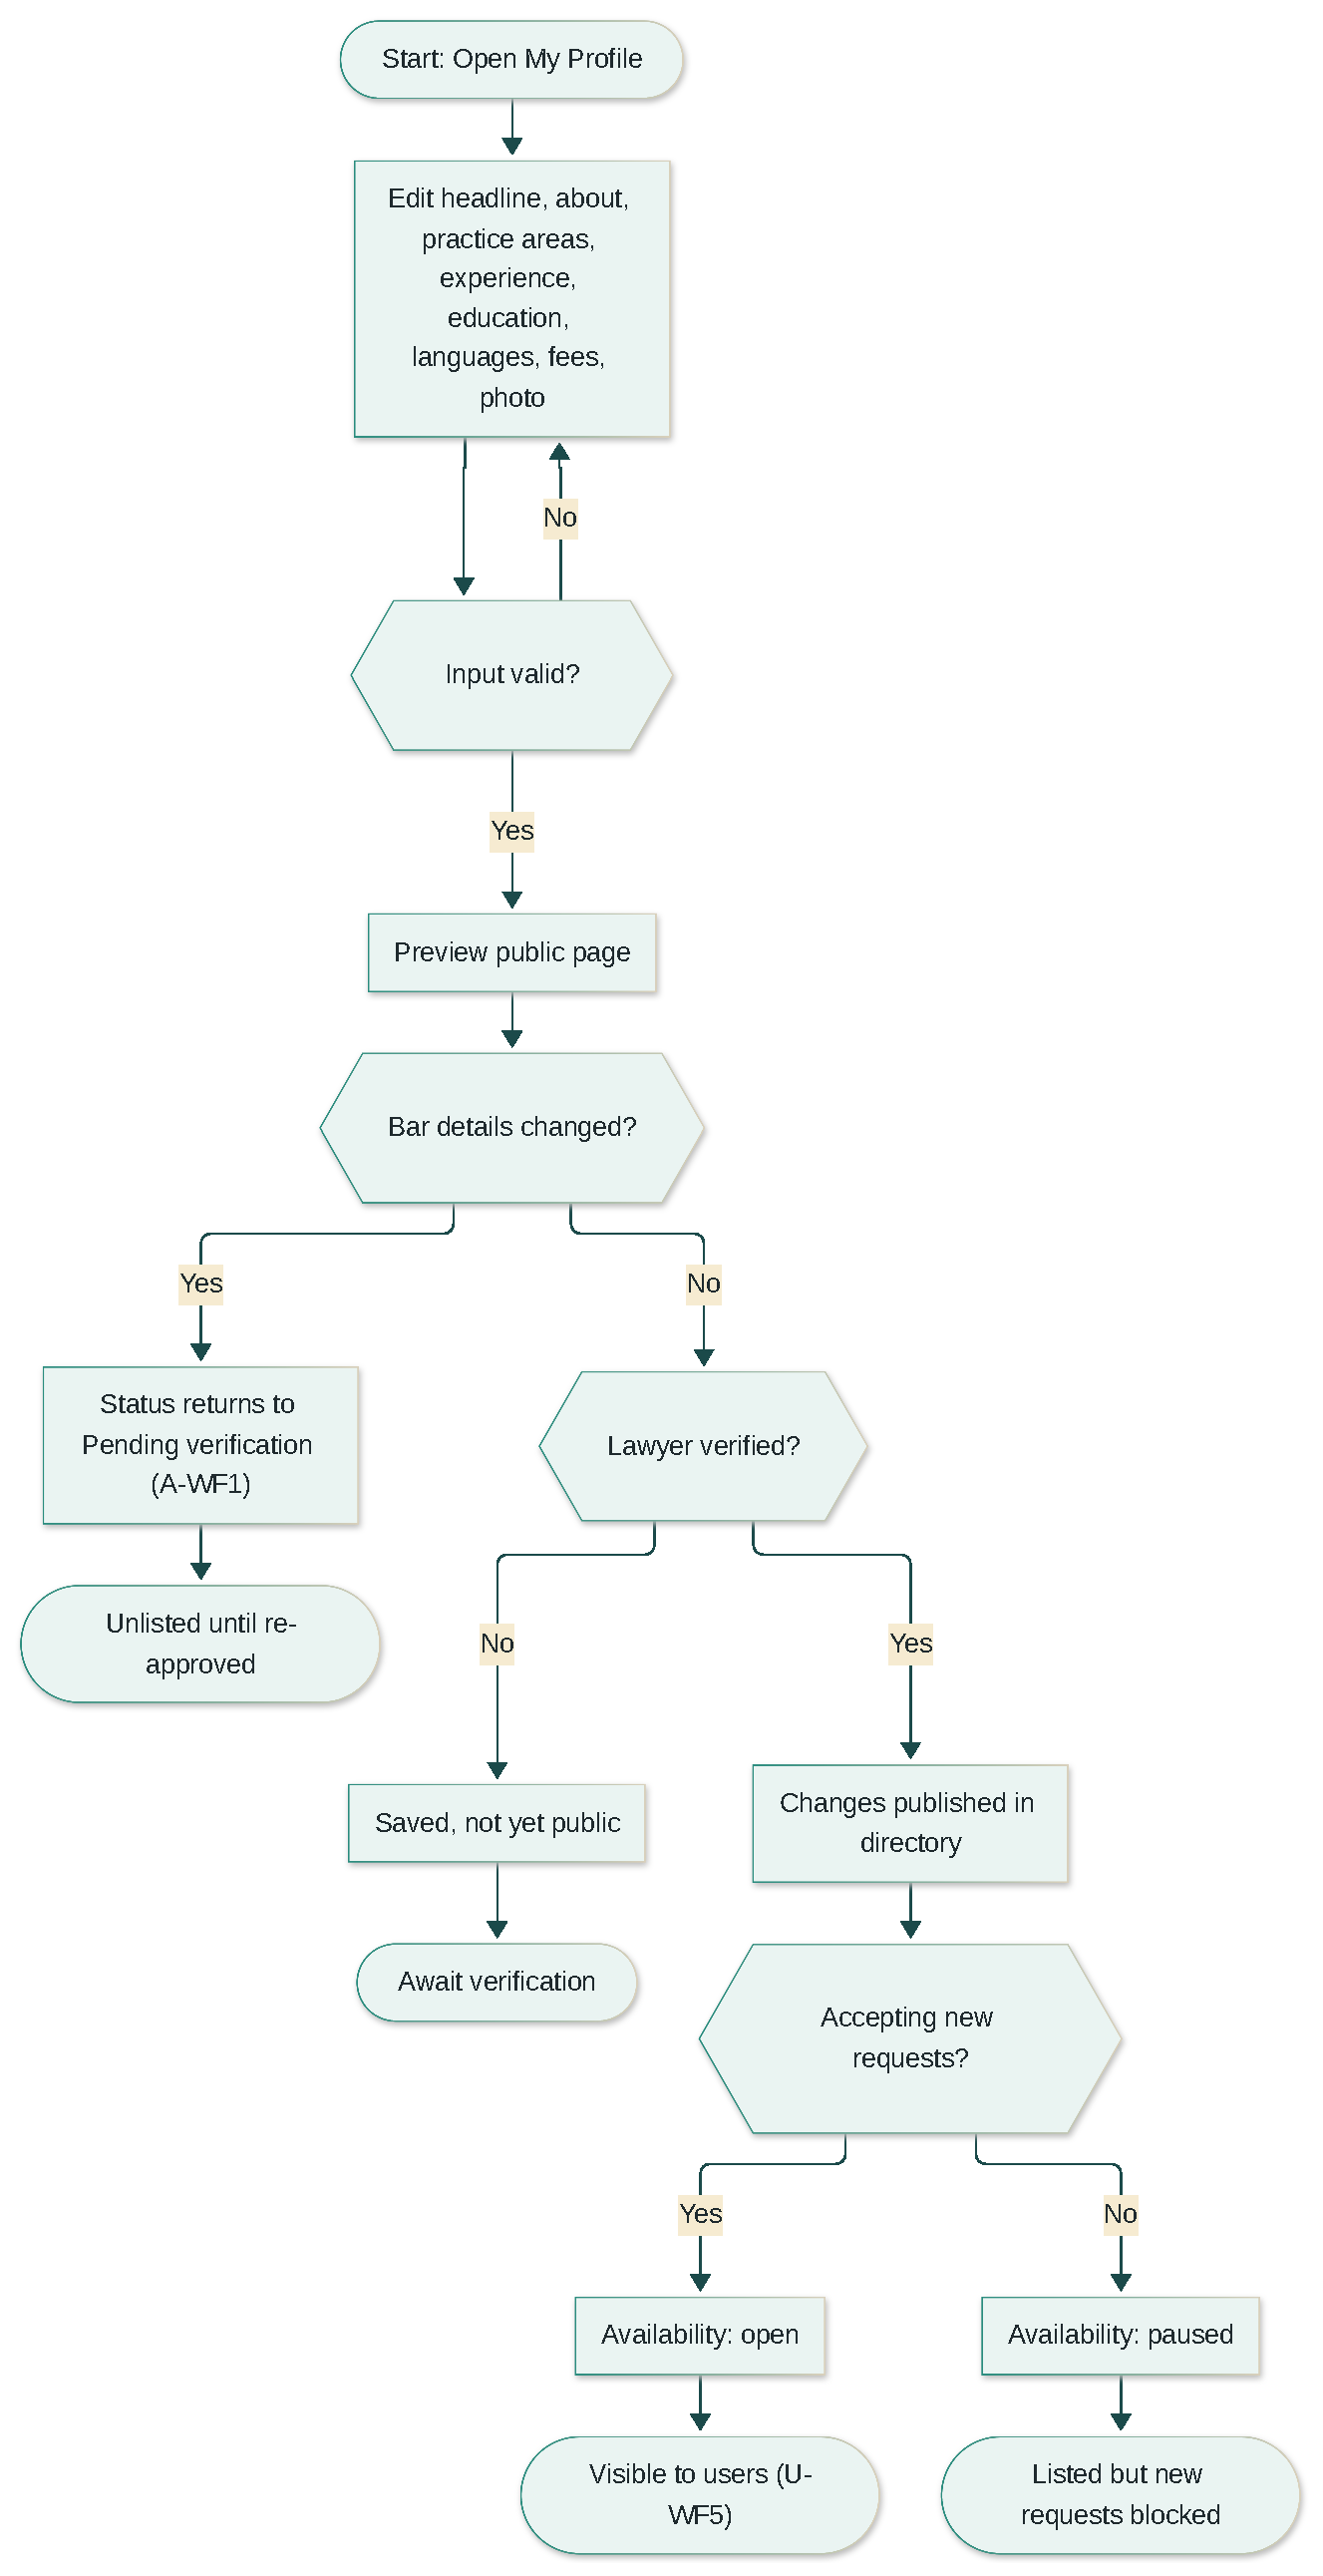
\includegraphics[width=\textwidth,height=0.80\textheight,keepaspectratio]{figures/wf_l2_profile.pdf}
\caption{L-WF2 Public profile and availability management}\label{fig:3.3}
\end{figure}

\needspace{12\baselineskip}
\section{L-WF3: Handle Consultation Requests}

Requests arrive only from users who gave consent (U-WF5). Before every read of the shared case, the system checks that consent is still active.

% Mermaid source:
% %% name: wf_l3_requests
% flowchart TD
%     S(["Start: New request notification"]) --> LST["Open request list"]
%     USR["User: consultation request + consent (U-WF5)"] -.-> LST
%     LST --> OPN["Open request"]
%     OPN --> CNS{{"Consent still active?"}}
%     CNS -->|No| CLS(["Request closed, case hidden"])
%     CNS -->|Yes| VIEW["Read case summary, guidance, documents, checklist"]
%     VIEW --> DEC{{"Decision"}}
%     DEC -->|Decline| DCL["Decline with optional reason"] --> N1["User notified, access ends"] --> E1(["End"])
%     DEC -->|Propose other time| PRP["Suggest new time"] --> UR{{"User accepts time?"}}
%     UR -->|No| CAN(["Consultation cancelled"])
%     UR -->|Yes| SCH
%     DEC -->|Accept| SCH["Status: Scheduled"]
%     SCH --> N2["User notified, contact details released"]
%     N2 --> E2(["Work on case (L-WF4)"])
\begin{figure}[H]\centering
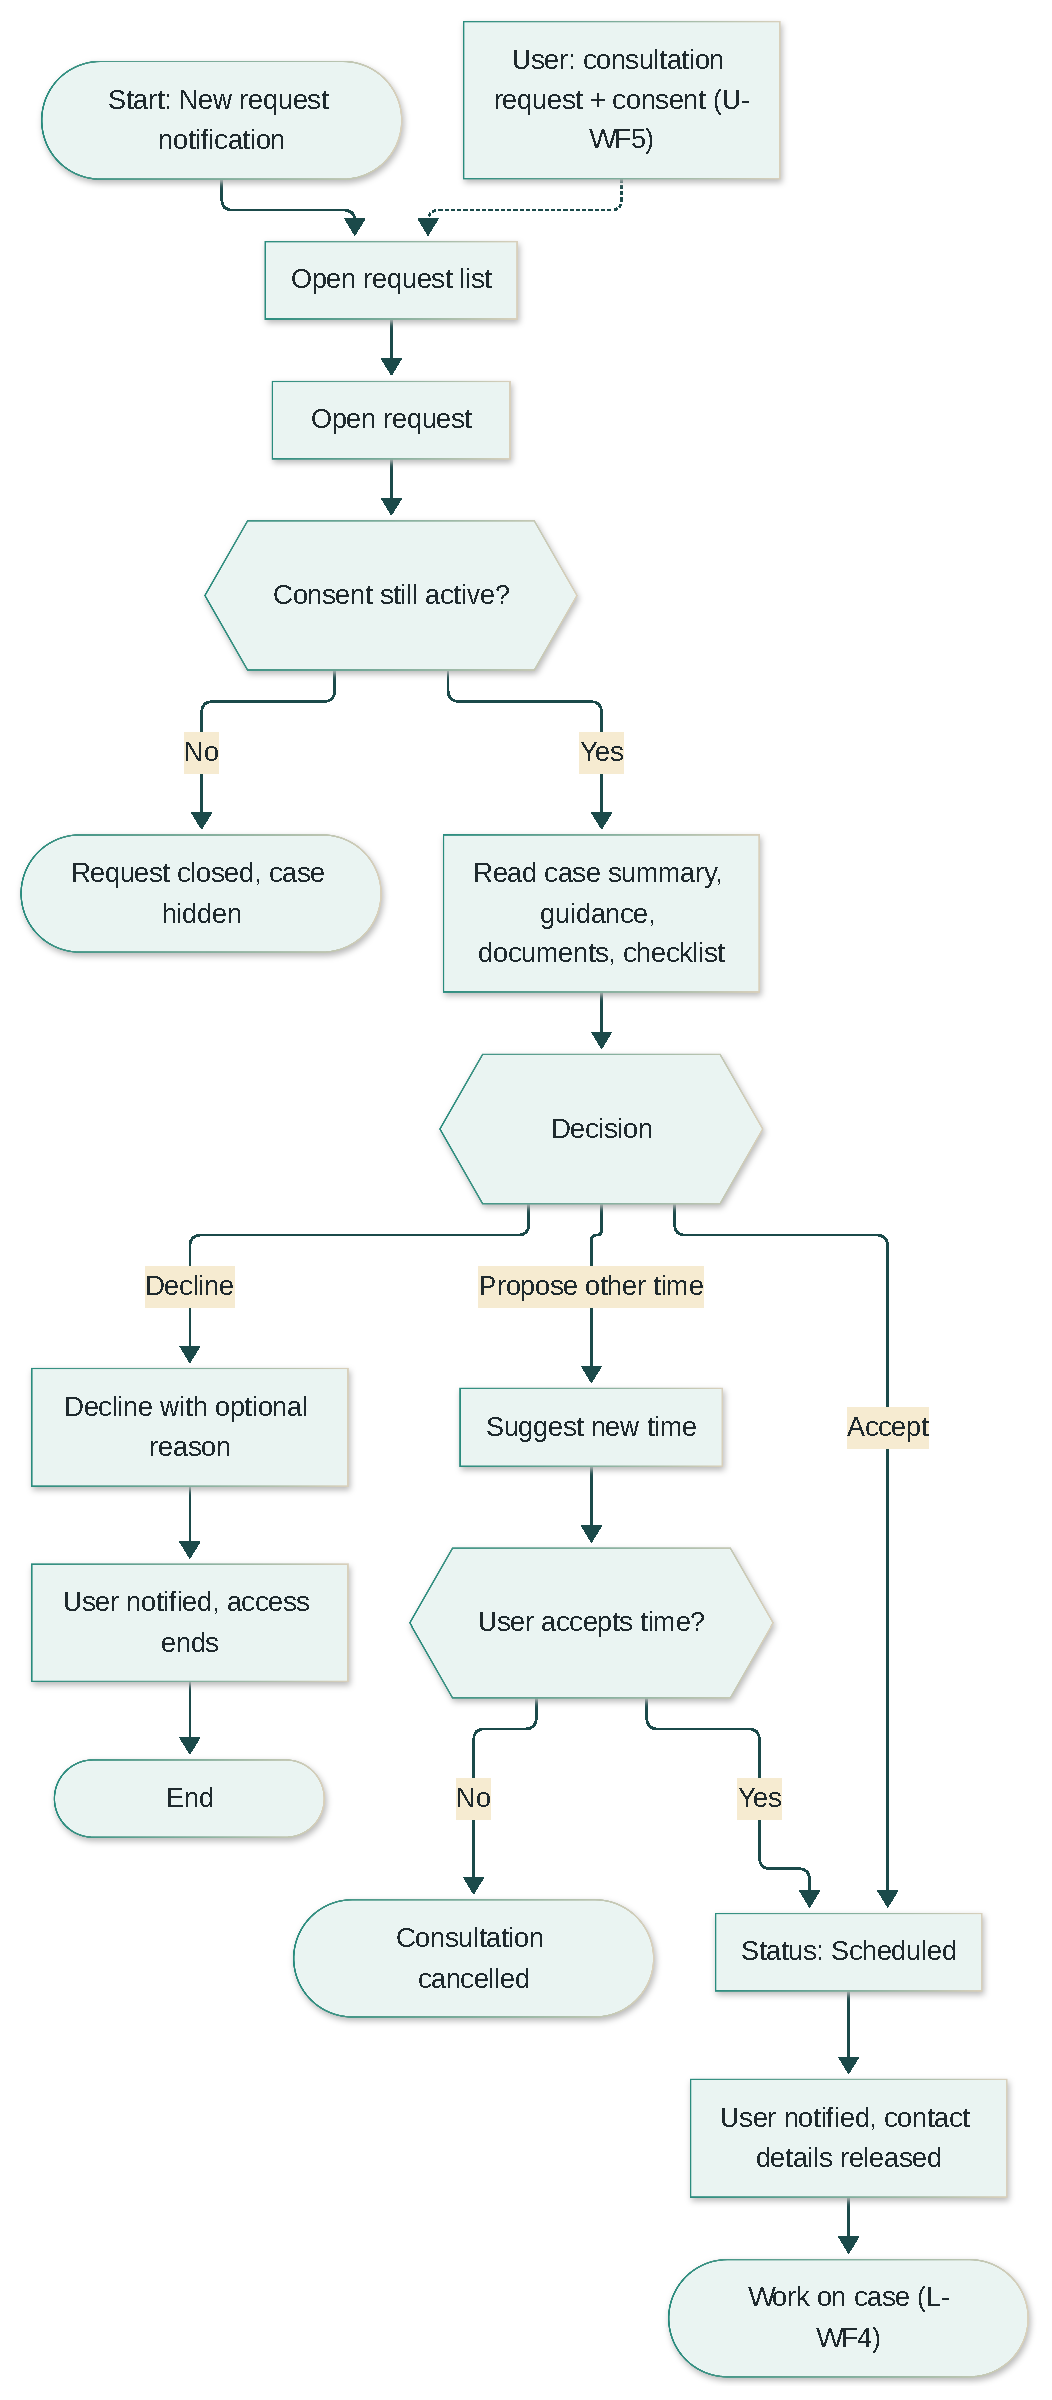
\includegraphics[width=\textwidth,height=0.80\textheight,keepaspectratio]{figures/wf_l3_requests.pdf}
\caption{L-WF3 Handle consultation requests}\label{fig:3.4}
\end{figure}

\needspace{12\baselineskip}
\section{L-WF4: Work on a Shared Case}

While the consultation is active, the lawyer exchanges messages and posts status updates that appear on the user's timeline (U-WF6). Completing the consultation enables the user's review.

% Mermaid source:
% %% name: wf_l4_casework
% flowchart TD
%     S(["Start: Consultation Scheduled"]) --> CS{{"Consent still active?"}}
%     CS -->|No| STOP(["Access ended by user revocation"])
%     CS -->|Yes| ACT{{"Choose action"}}
%     ACT -->|Message| MSG["Send message to user"] --> CS
%     ACT -->|Update| UPD["Post status update and note"] --> TL["Added to user timeline, user notified"] --> CS
%     ACT -->|Consultation held| CMP["Mark consultation Completed"]
%     CMP --> RV["User invited to review (U-WF6)"]
%     RV --> E(["End"])
\begin{figure}[H]\centering
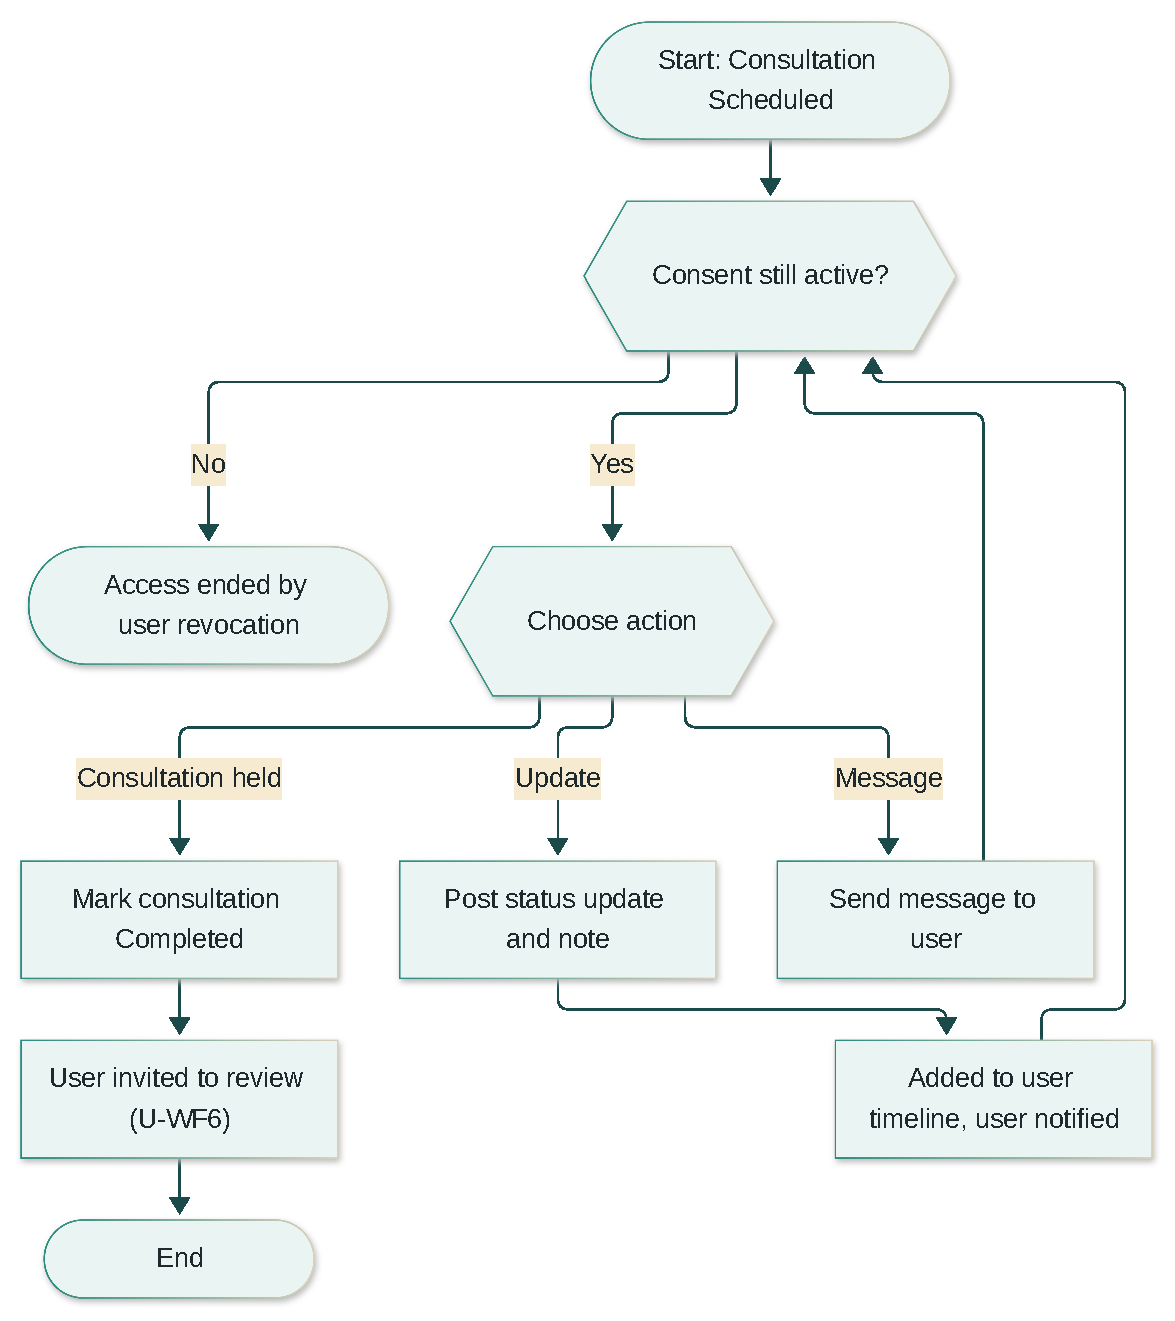
\includegraphics[width=\textwidth,height=0.80\textheight,keepaspectratio]{figures/wf_l4_casework.pdf}
\caption{L-WF4 Work on a shared case}\label{fig:3.5}
\end{figure}

\chapter{Admin Workflows}\label{ch:4}

\section{Admin Actions and Dependencies}

\begin{longtable}{|L{1.73cm}|L{4.48cm}|L{2.60cm}|L{3.03cm}|L{1.70cm}|}
\caption{Actions of the Admin and their dependencies}\label{tab:4.1}\\
\hline\headrow \thd{ID} & \thd{Action} & \thd{Depends on} & \thd{Result} & \thd{Req.} \\ \hline
\endfirsthead
\hline\headrow \thd{ID} & \thd{Action} & \thd{Depends on} & \thd{Result} & \thd{Req.} \\ \hline
\endhead
\hline\endlastfoot
A-A01 & Log in to Admin portal & Administrator role & Admin dashboard & AFR-01 \\ \hline
A-A02 & Review verification queue & Pending requests (L-WF1) & Request details and licence & AFR-02 \\ \hline
A-A03 & Approve, reject or request information & A-A02; external check with bar council records & Lawyer Verified / Rejected / Pending & AFR-02 \\ \hline
A-A04 & Add legal source with metadata & Official text available & Source Processing & AFR-05 \\ \hline
A-A05 & Review indexed chunks and verify source & A-A04; ingestion done (S-WF3) & Source Verified and retrievable & AFR-05, AFR-06 \\ \hline
A-A06 & Re-index amended source / retire repealed source & A-A05 & Updated or excluded from retrieval & AFR-07 \\ \hline
A-A07 & Search, view, suspend, reactivate, remove accounts & A-A01 & Account status changed & AFR-03 \\ \hline
A-A08 & Moderate reported profiles and reviews & Reports from users & Content kept or removed & AFR-04 \\ \hline
A-A09 & View platform statistics & A-A01 & Dashboard metrics & AFR-08 \\ \hline
A-A10 & View and filter audit log & Logged admin actions & Audit trail & AFR-09 \\
\end{longtable}

% Mermaid source:
% %% name: actions_admin
% flowchart TB
%     ROOT(["Admin"])
%     G1["<b>Lawyer verification</b>"]
%     ROOT --> G1
%     G1A1["Review queue and licence"]
%     G1 --> G1A1
%     G1A2["Approve / reject / request info"]
%     G1A1 ~~~ G1A2
%     G2["<b>Legal knowledge base</b>"]
%     ROOT --> G2
%     G2A1["Add source with metadata"]
%     G2 --> G2A1
%     G2A2["Review chunks and verify"]
%     G2A1 ~~~ G2A2
%     G2A3["Re-index or retire source"]
%     G2A2 ~~~ G2A3
%     G3["<b>Account management</b>"]
%     ROOT --> G3
%     G3A1["Search and view accounts"]
%     G3 --> G3A1
%     G3A2["Suspend / reactivate / remove"]
%     G3A1 ~~~ G3A2
%     G4["<b>Moderation</b>"]
%     ROOT --> G4
%     G4A1["Review reported content"]
%     G4 --> G4A1
%     G4A2["Keep or remove content"]
%     G4A1 ~~~ G4A2
%     G5["<b>Monitoring</b>"]
%     ROOT --> G5
%     G5A1["Platform statistics"]
%     G5 --> G5A1
%     G5A2["Audit log"]
%     G5A1 ~~~ G5A2
\begin{figure}[H]\centering
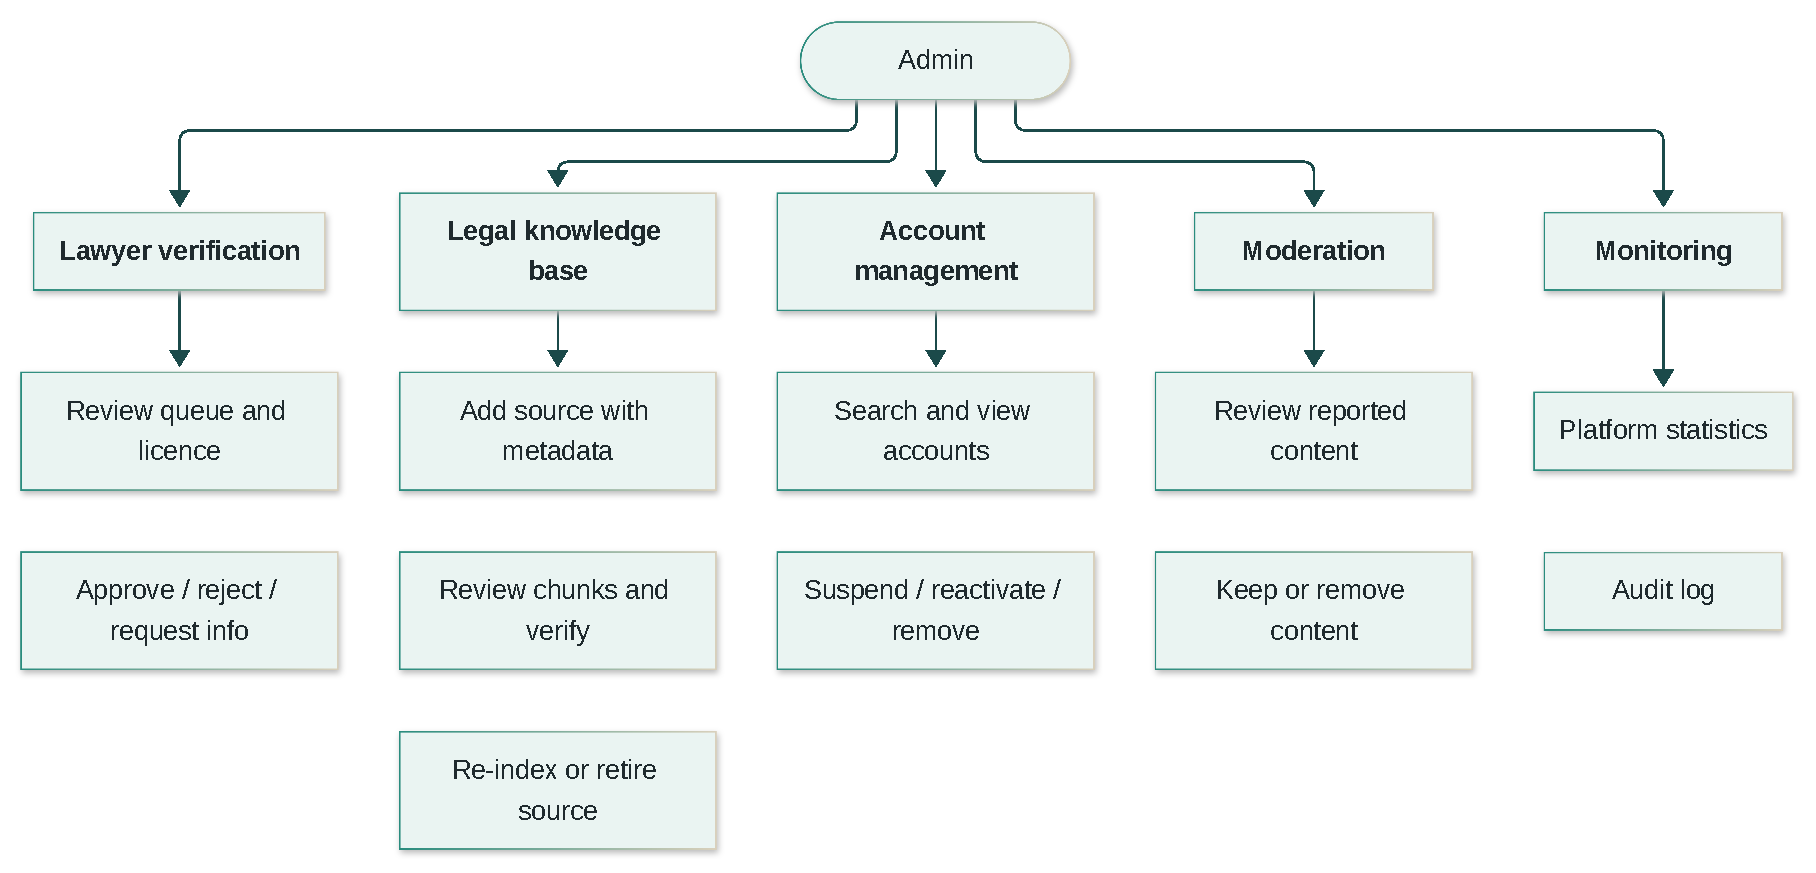
\includegraphics[width=\textwidth,height=0.80\textheight,keepaspectratio]{figures/actions_admin.pdf}
\caption{Actions available to the Admin}\label{fig:4.1}
\end{figure}

\needspace{12\baselineskip}
\section{A-WF1: Lawyer Verification}

The Admin checks each lawyer's bar enrolment details against the issuing bar council's records, which is done outside the system, and records the decision. The decision directly controls whether the lawyer appears in the user's directory (U-WF5).

% Mermaid source:
% %% name: wf_a1_verify
% flowchart TD
%     S(["Start"]) --> Q["Open verification queue"]
%     LW["Lawyer: verification request (L-WF1)"] -.-> Q
%     Q --> SEL["Select pending request"]
%     SEL --> DOC["View details and licence document"]
%     DOC --> EXT["Check against bar council records (outside system)"]
%     EXT --> M{{"Details match?"}}
%     M -->|Yes| AP["Approve: status Verified, profile listed"]
%     M -->|Unclear| INF["Request more information"] --> W(["Request stays pending"])
%     M -->|No| RJ["Reject with reason"]
%     AP --> LOG["Write audit log entry"]
%     RJ --> LOG
%     LOG --> NT["Notify lawyer (S-WF4)"]
%     NT --> MORE{{"More requests?"}}
%     MORE -->|Yes| SEL
%     MORE -->|No| E(["End"])
\begin{figure}[H]\centering
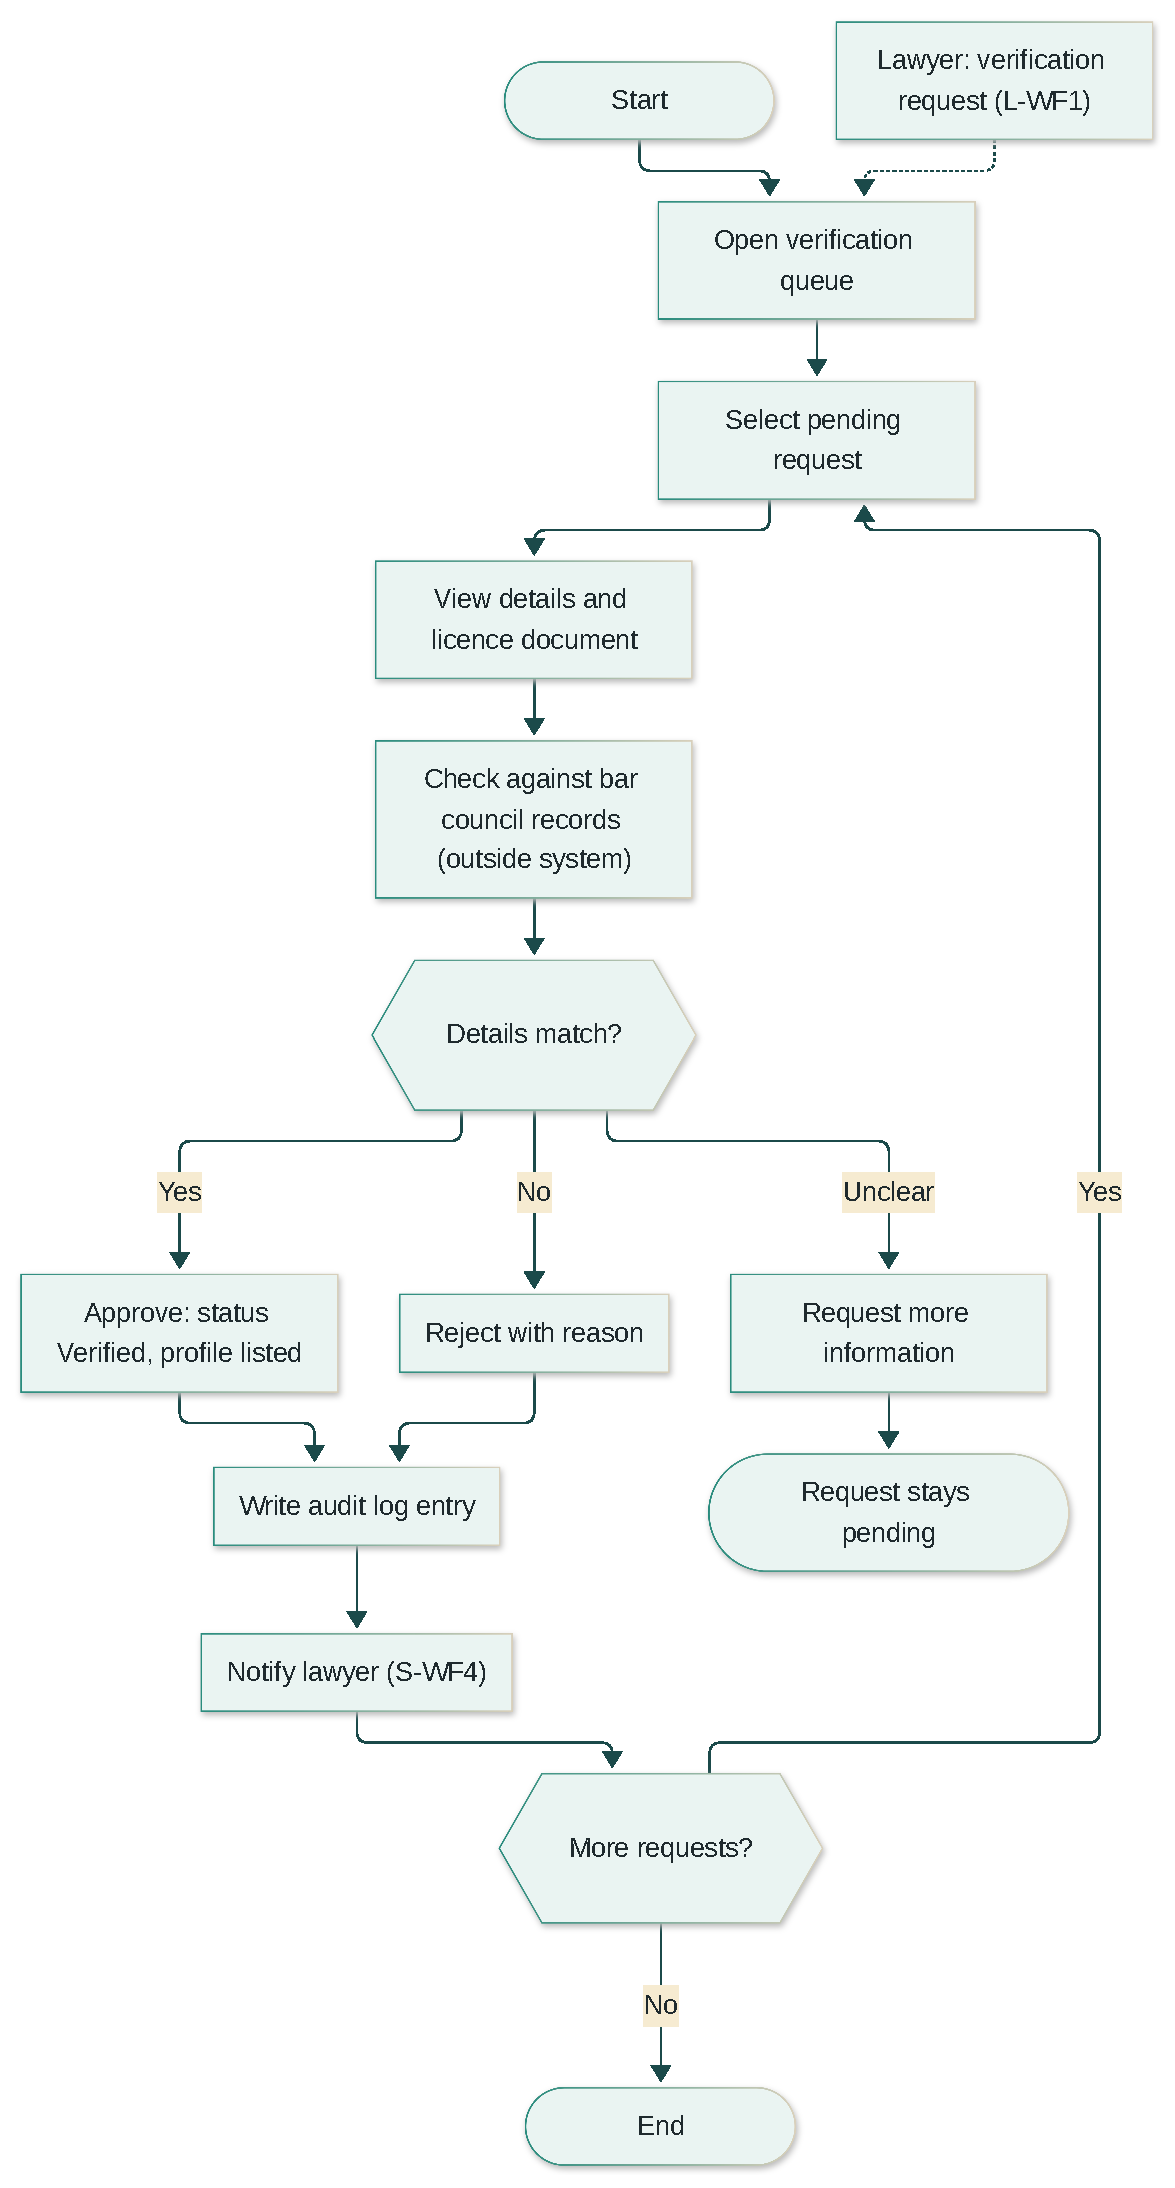
\includegraphics[width=\textwidth,height=0.80\textheight,keepaspectratio]{figures/wf_a1_verify.pdf}
\caption{A-WF1 Lawyer verification}\label{fig:4.2}
\end{figure}

\needspace{12\baselineskip}
\section{A-WF2: Legal Knowledge Base Management}

Only sources that the Admin has reviewed and verified are retrievable by the AI assistant. This is the key control that keeps guidance grounded in verified Pakistani law.

% Mermaid source:
% %% name: wf_a2_kb
% flowchart TD
%     S(["Start"]) --> ACT{{"Task"}}
%     ACT -->|Add source| UP["Upload official text and metadata: title, type, year, area, URL"]
%     UP --> ING["System ingestion (S-WF3)"]
%     ING --> RVW["Review sample of section chunks"]
%     RVW --> OK{{"Chunks correct?"}}
%     OK -->|No| FIX["Flag for manual correction and re-ingest"] --> ING
%     OK -->|Yes| VER["Mark source Verified"]
%     VER --> LIVE(["Retrievable by RAG pipeline (S-WF1)"])
%     ACT -->|Source amended| NEW["Upload new text"] --> REIDX["Re-index and retire old chunks"] --> RVW
%     ACT -->|Source repealed| RET["Retire source"] --> EX(["Excluded from retrieval, kept for past citations"])
\begin{figure}[H]\centering
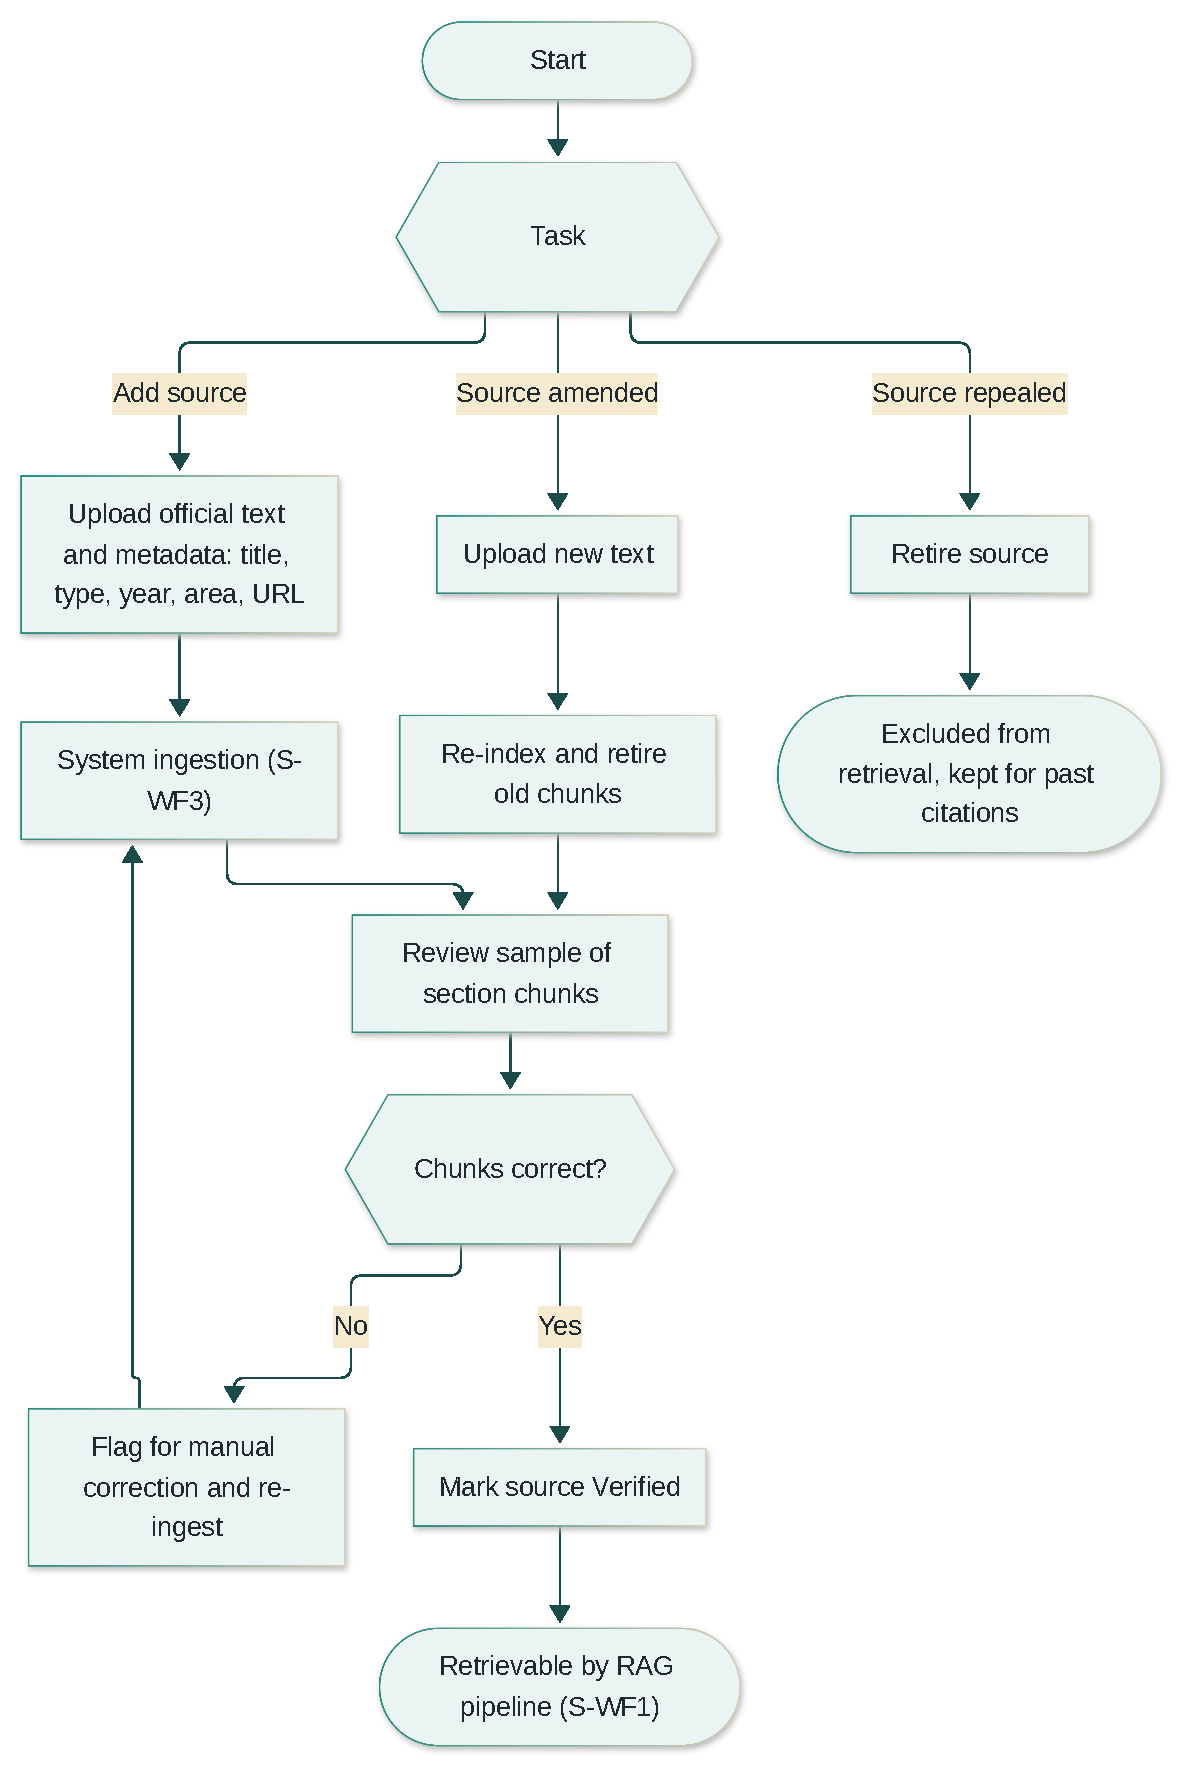
\includegraphics[width=\textwidth,height=0.80\textheight,keepaspectratio]{figures/wf_a2_kb.pdf}
\caption{A-WF2 Legal knowledge base management}\label{fig:4.3}
\end{figure}

\needspace{12\baselineskip}
\section{A-WF3: User and Lawyer Account Management}

% Mermaid source:
% %% name: wf_a3_accounts
% flowchart TD
%     S(["Start"]) --> SR["Search account by name, email or role"]
%     SR --> VW["Open account details"]
%     VW --> D{{"Action"}}
%     D -->|Suspend| SU["Suspend with reason"] --> SES["End active sessions"] --> LOG
%     D -->|Reactivate| RA["Reactivate account"] --> LOG
%     D -->|Remove| RM["Remove or anonymise account"] --> LOG
%     D -->|No action| E0(["End"])
%     LOG["Write audit log entry"] --> NT["Notify account holder"] --> E(["End"])
\begin{figure}[H]\centering
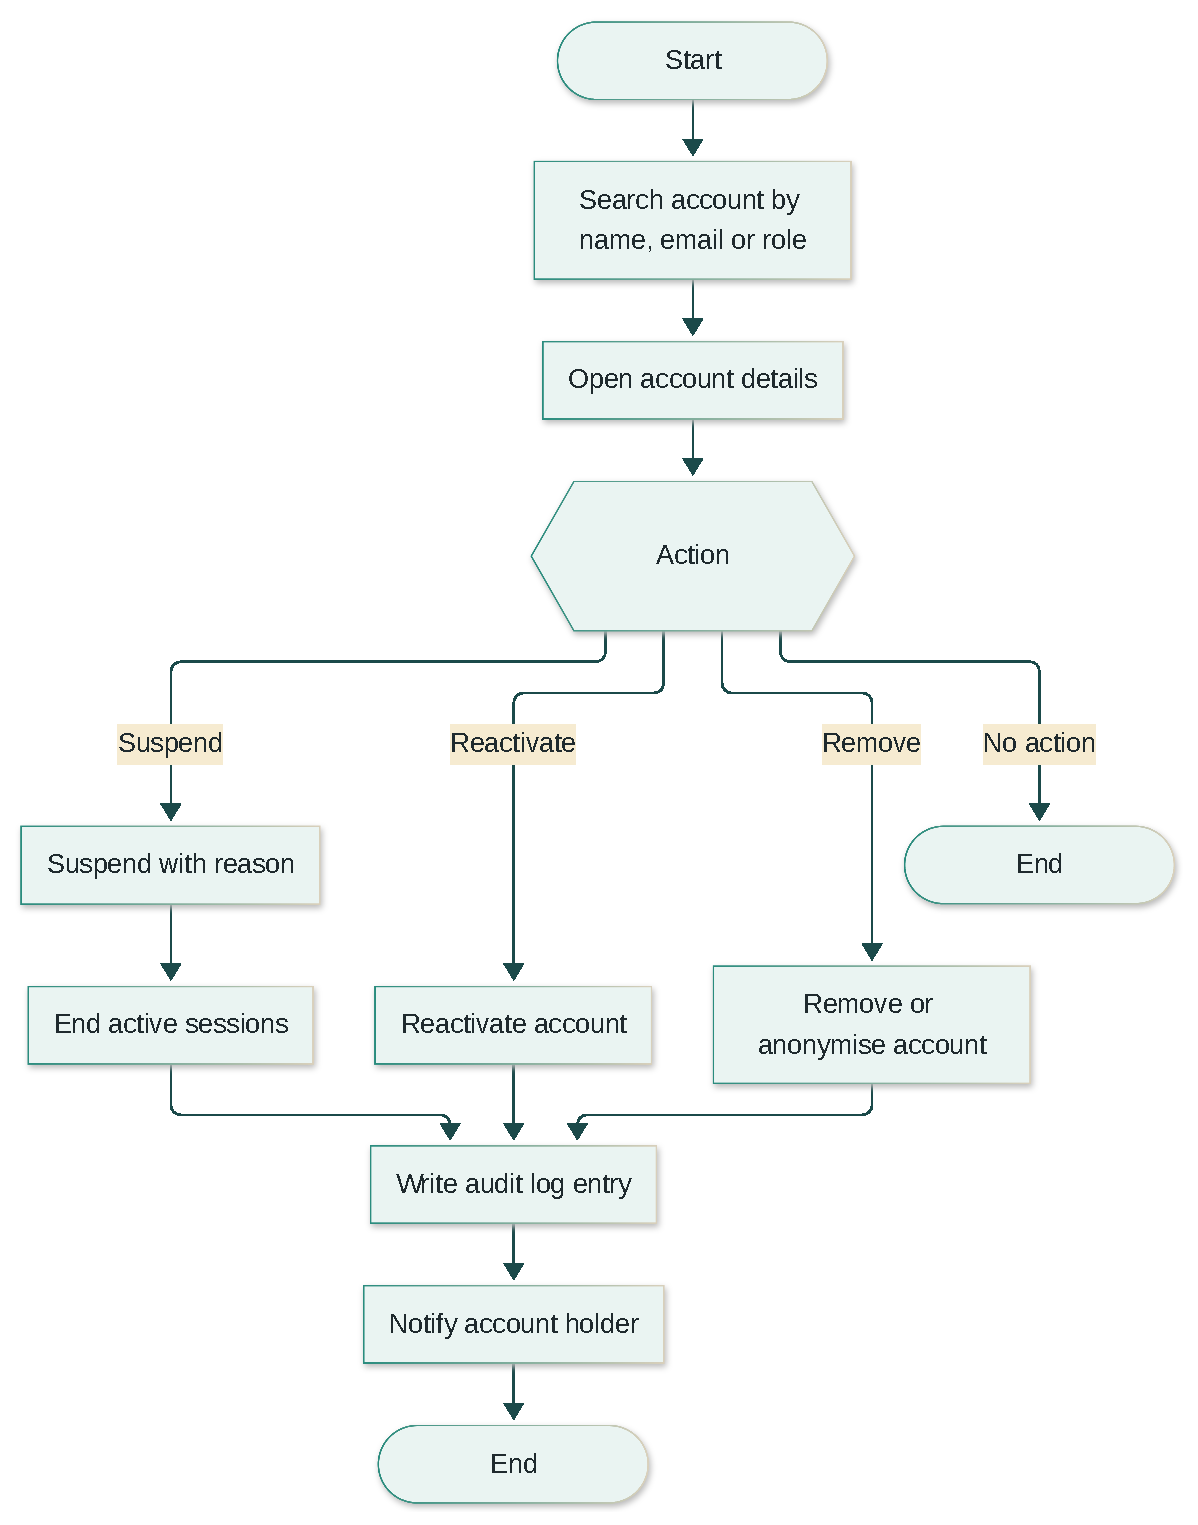
\includegraphics[width=\textwidth,height=0.80\textheight,keepaspectratio]{figures/wf_a3_accounts.pdf}
\caption{A-WF3 User and lawyer account management}\label{fig:4.4}
\end{figure}

Suspension takes effect immediately in U-WF1 and L-WF1: a suspended account cannot log in, and a suspended lawyer is removed from the directory.

\needspace{12\baselineskip}
\section{A-WF4: Content Moderation}

% Mermaid source:
% %% name: wf_a4_moderation
% flowchart TD
%     S(["Start"]) --> RQ["Open reports queue"]
%     USR["User reports profile item or review"] -.-> RQ
%     RQ --> IT["Select reported item"]
%     IT --> CHK{{"Violates platform rules?"}}
%     CHK -->|No| KEEP["Keep content, close report"]
%     CHK -->|Yes| REM["Remove content"]
%     REM --> SEV{{"Repeated or serious?"}}
%     SEV -->|Yes| SUS["Suspend account (A-WF3)"]
%     SEV -->|No| WARN["Notify content owner"]
%     KEEP --> LOG["Write audit log entry"]
%     SUS --> LOG
%     WARN --> LOG
%     LOG --> E(["End"])
\begin{figure}[H]\centering
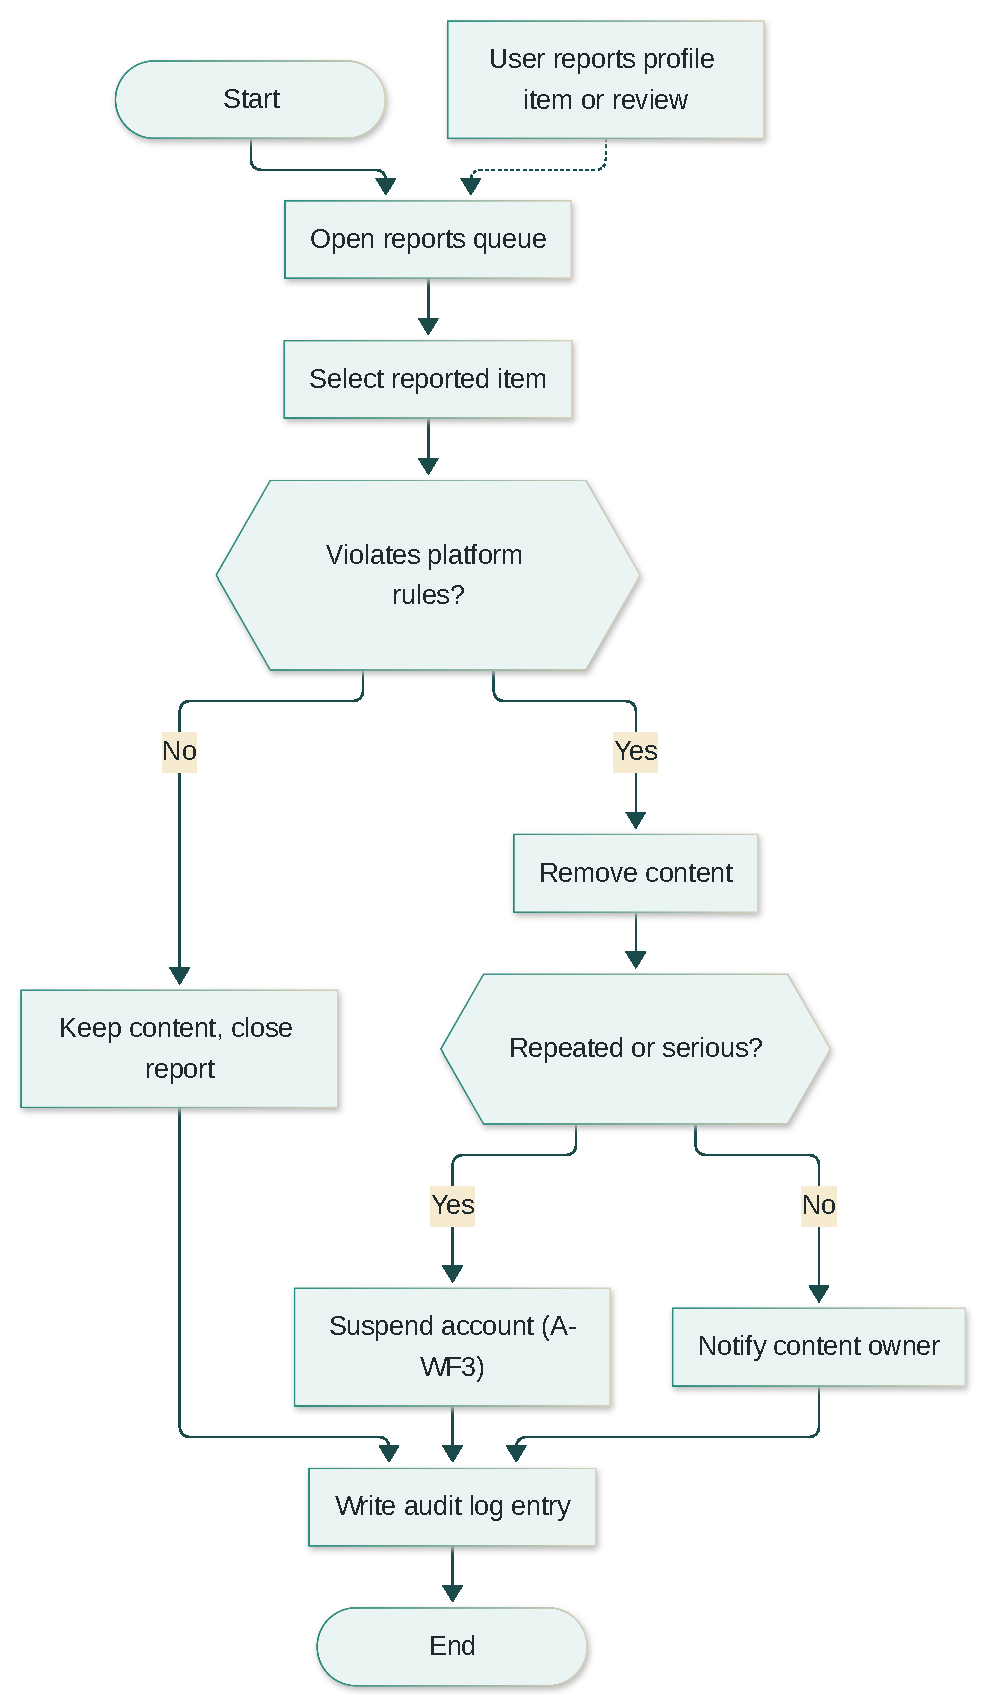
\includegraphics[width=\textwidth,height=0.80\textheight,keepaspectratio]{figures/wf_a4_moderation.pdf}
\caption{A-WF4 Content moderation}\label{fig:4.5}
\end{figure}

\needspace{12\baselineskip}
\section{A-WF5: Monitoring and Audit}

% Mermaid source:
% %% name: wf_a5_monitor
% flowchart TD
%     S(["Start"]) --> DB["Open admin dashboard"]
%     DB --> ST["View users, verified lawyers, open cases, consultations, indexed sections, guidance requests"]
%     ST --> WR{{"Withheld-answer rate high?"}}
%     WR -->|Yes| GAP["Identify missing topics"] --> KB(["Add sources (A-WF2)"])
%     WR -->|No| AUD{{"Audit review needed?"}}
%     AUD -->|Yes| FL["Filter audit log by date, admin, action"] --> RPT["Review actions"] --> E1(["End"])
%     AUD -->|No| E2(["End"])
\begin{figure}[H]\centering
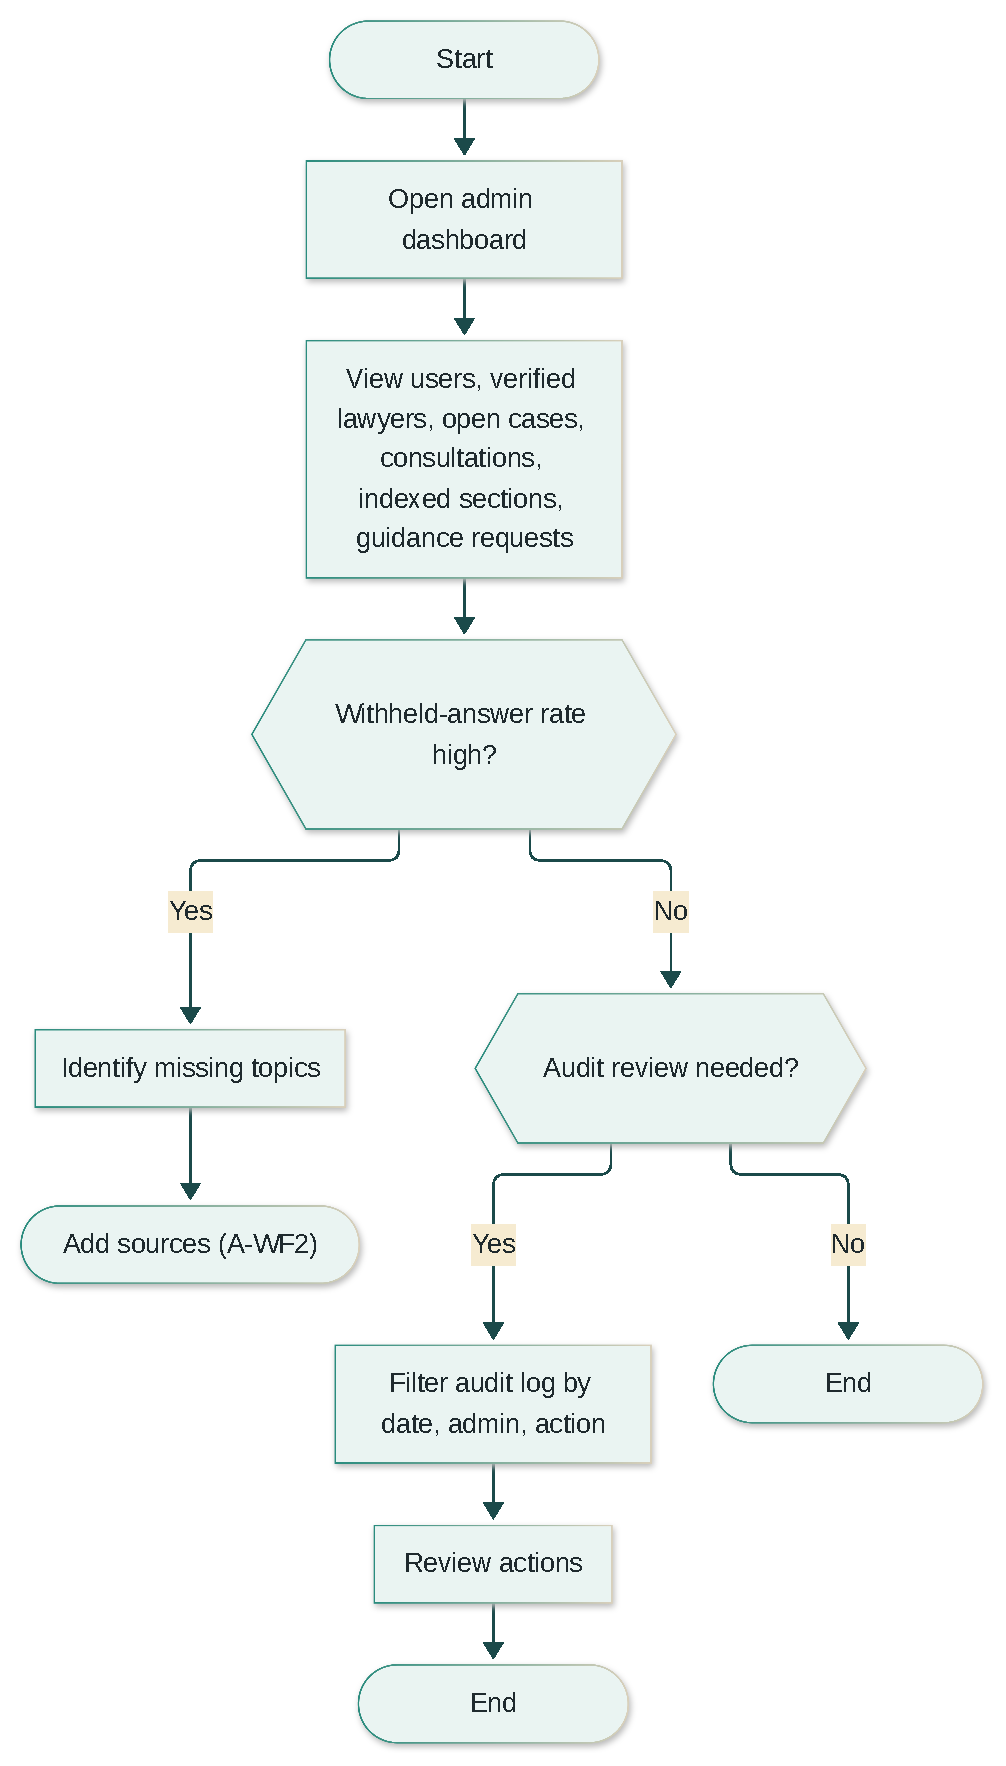
\includegraphics[width=\textwidth,height=0.80\textheight,keepaspectratio]{figures/wf_a5_monitor.pdf}
\caption{A-WF5 Monitoring and audit}\label{fig:4.6}
\end{figure}

A high rate of withheld (``no verified source'') answers signals gaps in the knowledge base, which the Admin closes by adding sources in A-WF2.

\chapter{System (AI Services) Workflows}\label{ch:5}

The system workflows run automatically when a human actor triggers them. They are shown as swimlanes across the backend components.

\needspace{12\baselineskip}
\section{S-WF1: RAG Guidance Pipeline}

Triggered by U-A10 and U-A11. The LLM receives only the retrieved sections, and no answer is shown unless its citations pass verification.

% Mermaid source:
% %% name: wf_s1_rag
% flowchart TD
%     S(["Guidance requested"]) --> F["RAG Service: load case facts and history"]
%     F --> EMB["Sentence Transformers: embed query"]
%     EMB --> QD["Qdrant: top-k similarity search filtered by legal area"]
%     KB["Verified sources only (A-WF2)"] -.-> QD
%     QD --> TH{{"Any section above relevance threshold?"}}
%     TH -->|No| NS(["Return: no verified source, suggest lawyer"])
%     TH -->|Yes| PR["Build grounded prompt: rules + sections + facts"]
%     PR --> LLM["Open-source LLM: generate answer with source tags"]
%     LLM --> CC{{"Citation checker: every statement tagged and every tag retrieved?"}}
%     CC -->|Yes| SAVE["Save guidance, citations, checklist"] --> OUT(["Return answer with sources and disclaimer"])
%     CC -->|No| RG{{"Already regenerated once?"}}
%     RG -->|No| LLM
%     RG -->|Yes| WH(["Answer withheld, user informed"])
\begin{figure}[H]\centering
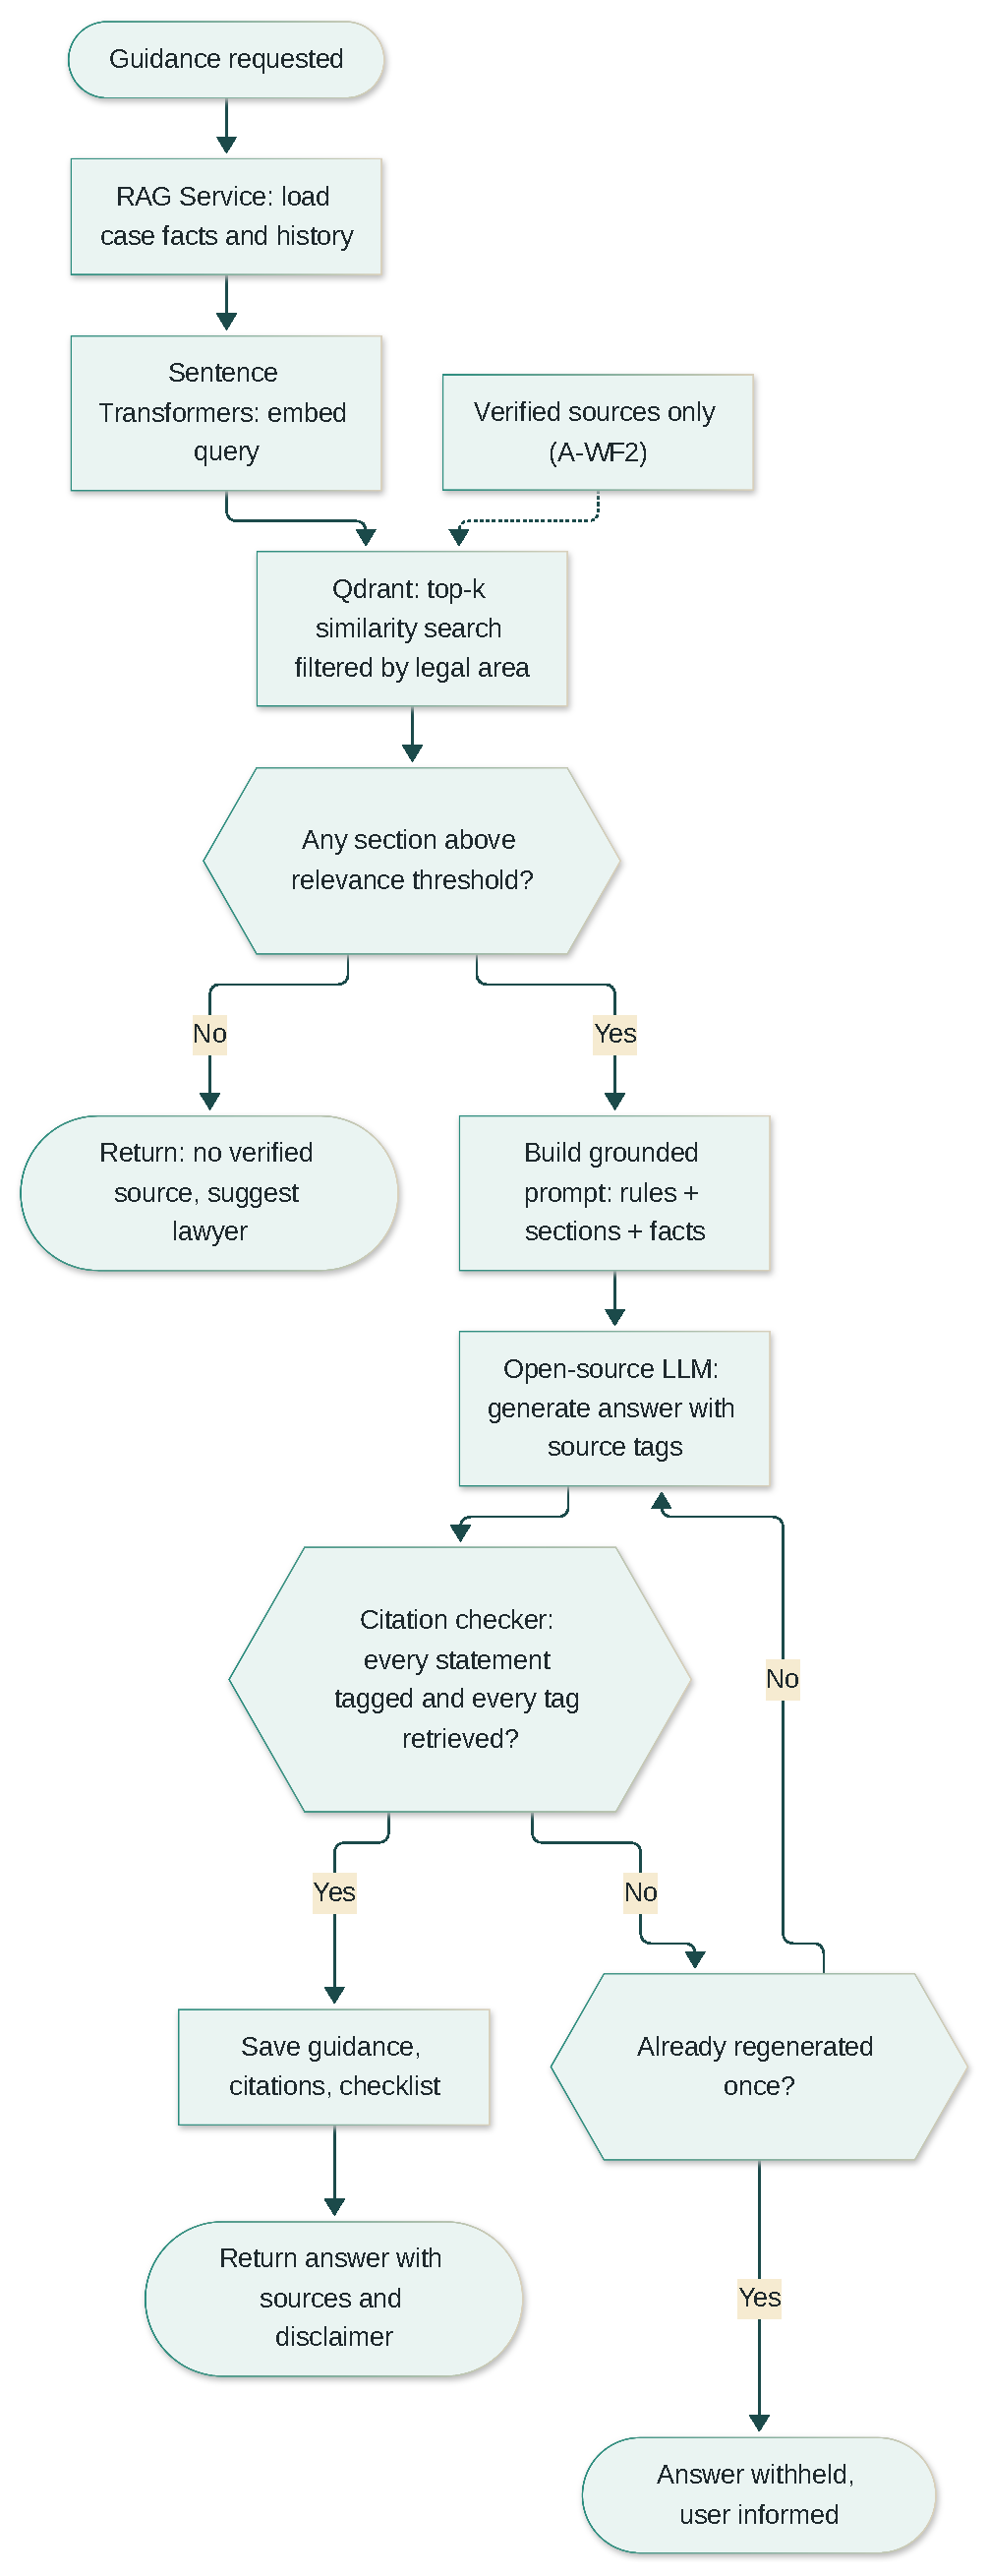
\includegraphics[width=\textwidth,height=0.80\textheight,keepaspectratio]{figures/wf_s1_rag.pdf}
\caption{S-WF1 RAG guidance pipeline}\label{fig:5.1}
\end{figure}

\needspace{12\baselineskip}
\section{S-WF2: Document Processing Pipeline}

Triggered by U-A12. Runs asynchronously so the user is not blocked.

% Mermaid source:
% %% name: wf_s2_docs
% flowchart TD
%     S(["File uploaded"]) --> V{{"Valid type and size?"}}
%     V -->|No| R(["Reject upload"])
%     V -->|Yes| ST["Store file, status Processing"]
%     ST --> TL{{"PDF with text layer?"}}
%     TL -->|Yes| PY["PyMuPDF: extract text"]
%     TL -->|No| OCR["OCR engine: recognise text"]
%     PY --> QL{{"Text quality acceptable?"}}
%     OCR --> QL
%     QL -->|No| LQ(["Mark Low quality, ask for clearer image"])
%     QL -->|Yes| CL["LLM: extract key clauses as structured fields"]
%     CL --> LK["Link document to case, match checklist items"]
%     LK --> NT(["Notify user: processing complete"])
\begin{figure}[H]\centering
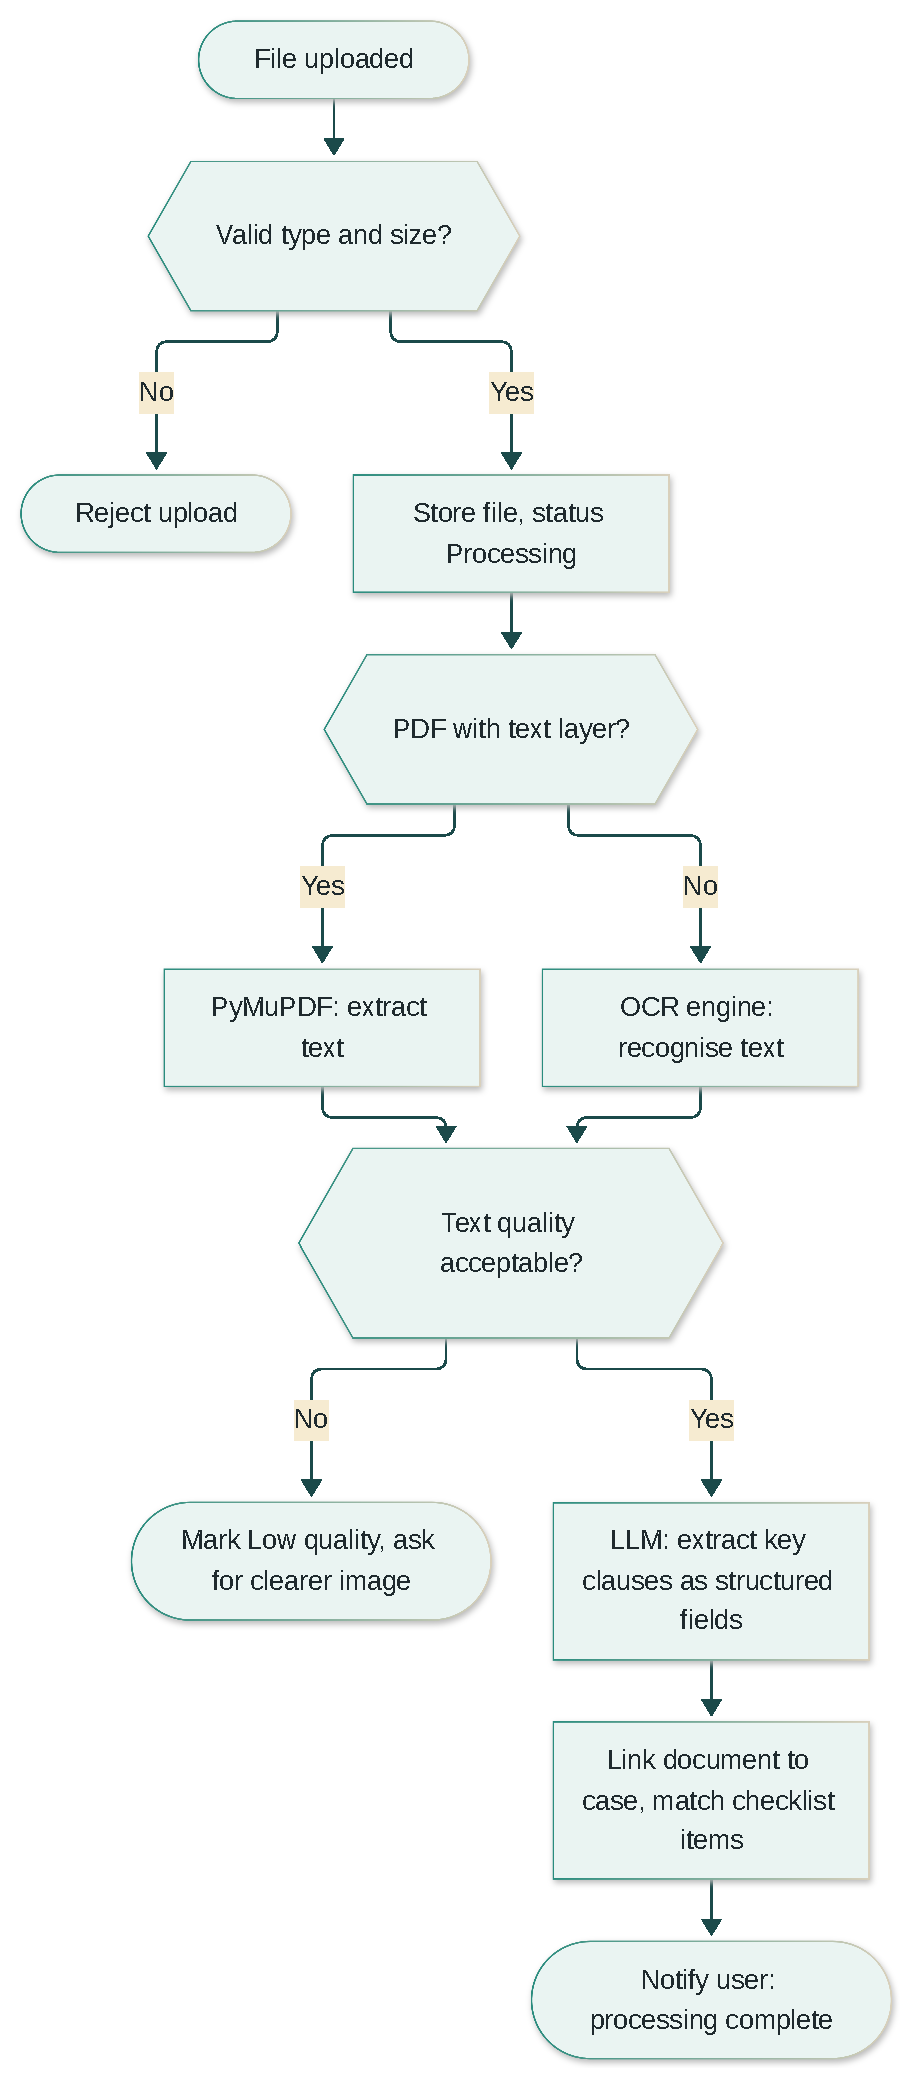
\includegraphics[width=\textwidth,height=0.80\textheight,keepaspectratio]{figures/wf_s2_docs.pdf}
\caption{S-WF2 Document processing pipeline}\label{fig:5.2}
\end{figure}

\needspace{12\baselineskip}
\section{S-WF3: Knowledge Base Ingestion Pipeline}

Triggered by A-A04 and A-A06.

% Mermaid source:
% %% name: wf_s3_ingest
% flowchart TD
%     S(["Source uploaded by Admin"]) --> EX["Extract text (PyMuPDF or OCR)"]
%     EX --> SEC{{"Section structure detected?"}}
%     SEC -->|Yes| CH["Split into section-wise chunks with metadata"]
%     SEC -->|No| FB["Fixed-length chunks with overlap, flag for review"]
%     CH --> LOOP["For each chunk"]
%     FB --> LOOP
%     LOOP --> EMB["Sentence Transformers: embed chunk"]
%     EMB --> UP["Qdrant: upsert vector with payload (chunk id, area, topic)"]
%     UP --> DB["MongoDB: store chunk record"]
%     DB --> MORE{{"More chunks?"}}
%     MORE -->|Yes| LOOP
%     MORE -->|No| AW(["Source status: Awaiting review (A-WF2)"])
\begin{figure}[H]\centering
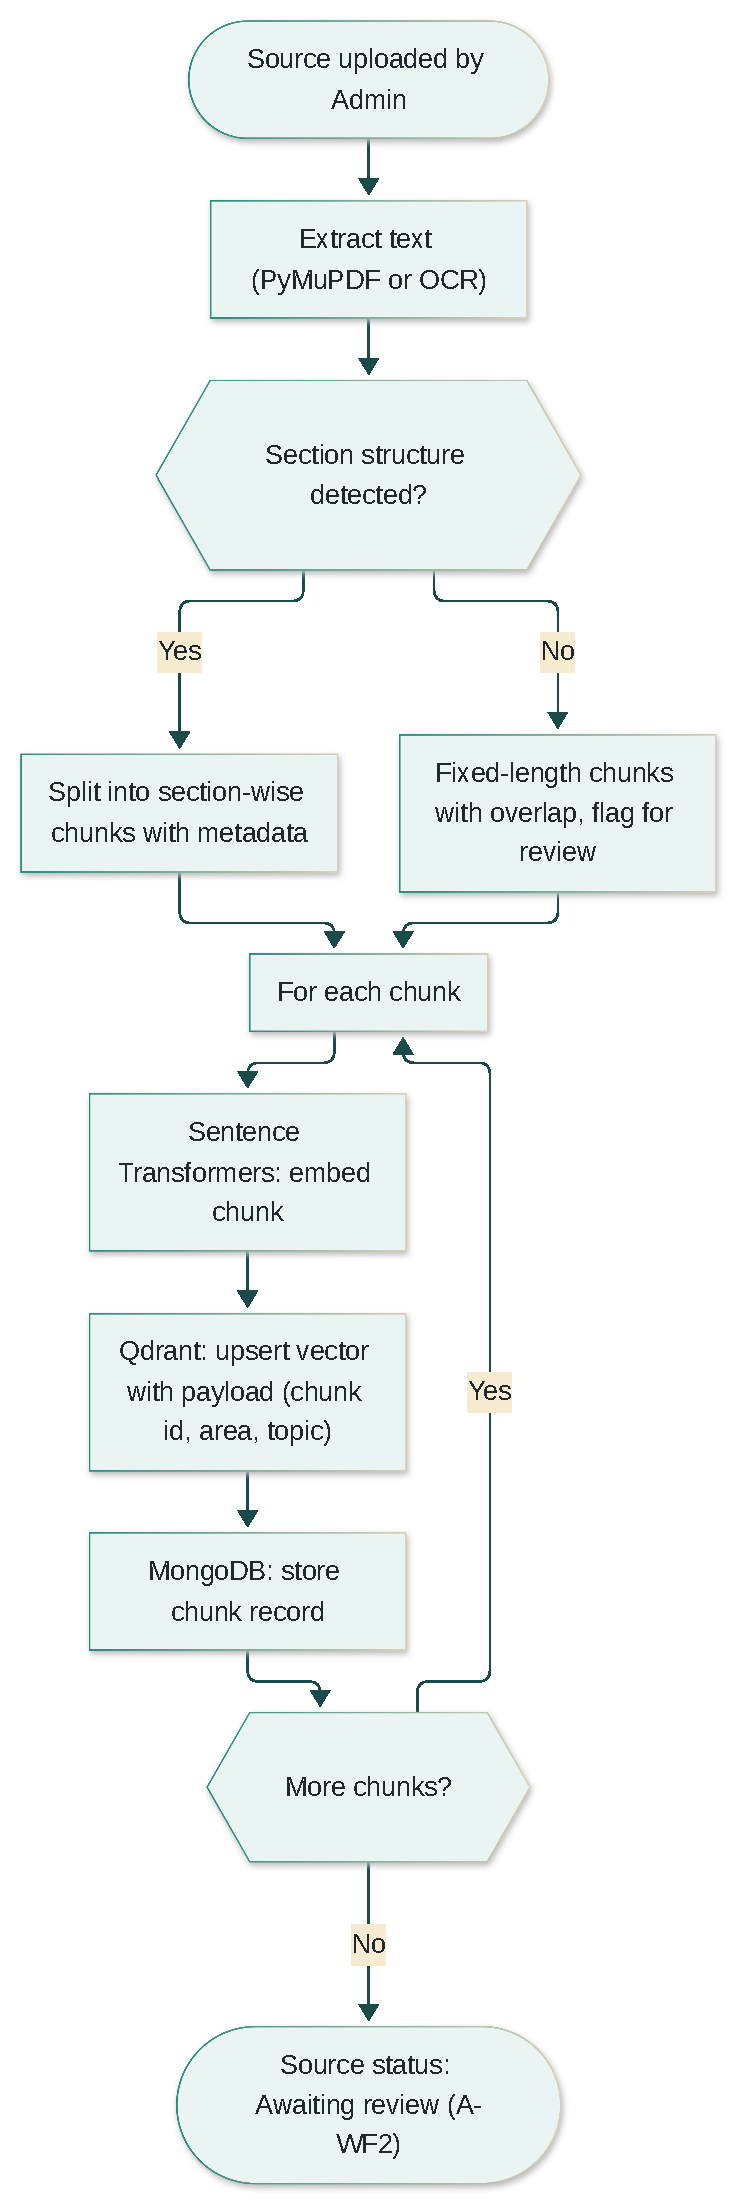
\includegraphics[width=\textwidth,height=0.80\textheight,keepaspectratio]{figures/wf_s3_ingest.pdf}
\caption{S-WF3 Knowledge base ingestion pipeline}\label{fig:5.3}
\end{figure}

\needspace{12\baselineskip}
\section{S-WF4: Notification Dispatch}

% Mermaid source:
% %% name: wf_s4_notify
% flowchart TD
%     S(["Event occurs"]) --> T{{"Event type"}}
%     T -->|Consultation requested| L1["Notify lawyer"]
%     T -->|Accepted, declined, rescheduled| U1["Notify user"]
%     T -->|Status update posted| U2["Notify user"]
%     T -->|Verification decision| L2["Notify lawyer"]
%     T -->|Account suspended or reactivated| A1["Notify account holder"]
%     L1 --> CH
%     U1 --> CH
%     U2 --> CH
%     L2 --> CH
%     A1 --> CH
%     CH["Create in-app notification"] --> EP{{"Email enabled for recipient?"}}
%     EP -->|Yes| EM["Send email"] --> E(["Done"])
%     EP -->|No| E
\begin{figure}[H]\centering
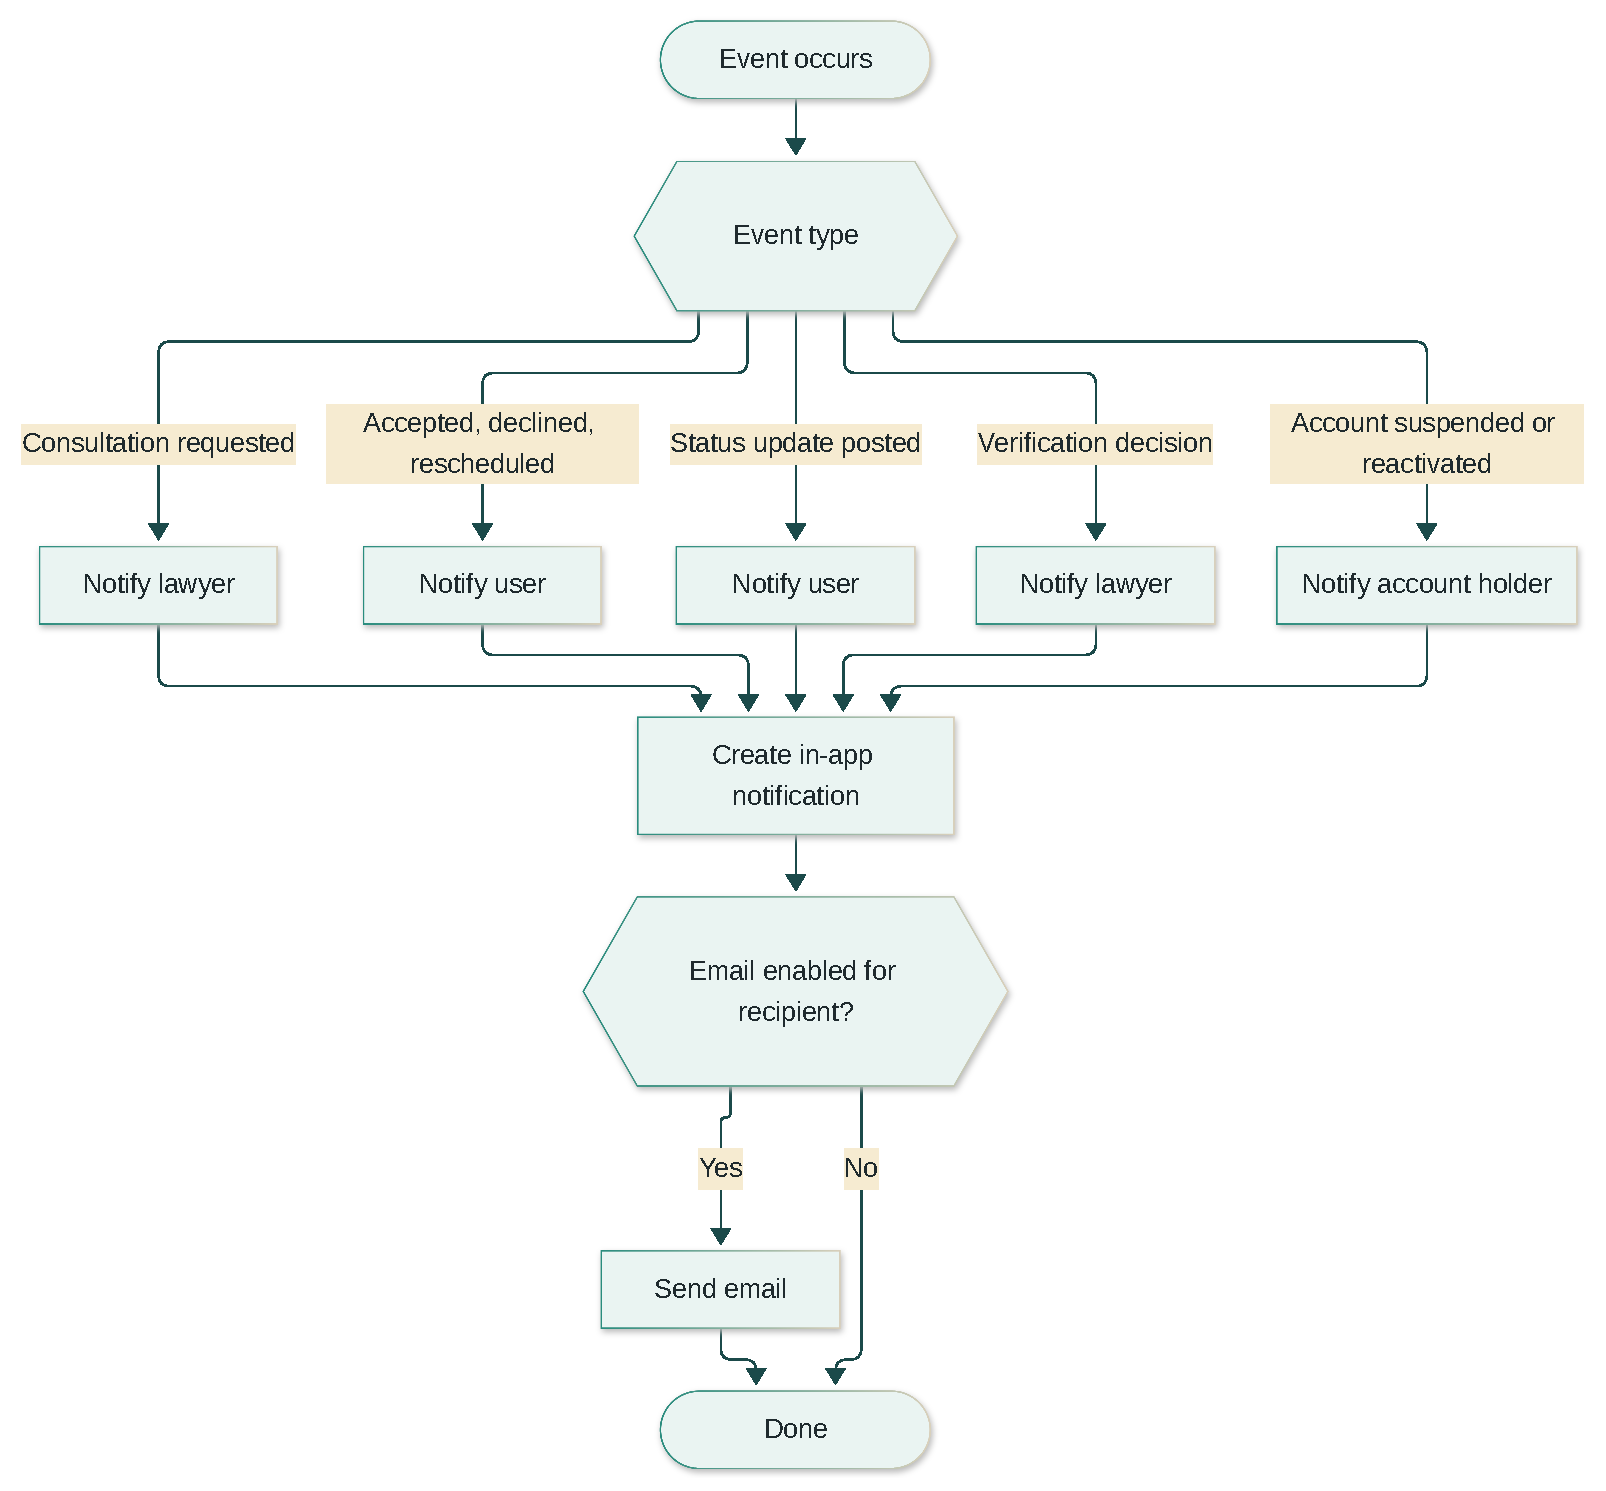
\includegraphics[width=\textwidth,height=0.80\textheight,keepaspectratio]{figures/wf_s4_notify.pdf}
\caption{S-WF4 Notification dispatch}\label{fig:5.4}
\end{figure}

\chapter{Cross-Actor Dependencies and Status Lifecycles}\label{ch:6}

\section{Dependency Graph}

Figure~\ref{fig:6.1} shows which workflow outcomes must exist before another workflow can proceed. Arrows point from the prerequisite to the dependent step. Two chains start with the Admin. The \textbf{knowledge chain} (A-WF2 to S-WF3 to S-WF1) makes AI guidance possible. The \textbf{trust chain} (L-WF1 to A-WF1 to L-WF2 to U-WF5) makes lawyers discoverable. The consultation then depends on both the user's case and the user's consent.

% Mermaid source:
% %% name: dependency_graph
% %% landscape
% flowchart LR
%     subgraph ADMIN["Admin"]
%         AKB["A-WF2 Verify legal sources"]
%         AVL["A-WF1 Approve lawyer"]
%         AAC["A-WF3 Account status"]
%     end
%     subgraph SYSTEM["AI Services"]
%         SIN["S-WF3 Index sources in Qdrant"]
%         SRAG["S-WF1 RAG pipeline"]
%         SDOC["S-WF2 Document processing"]
%     end
%     subgraph USER["User"]
%         UACC["U-WF1 Active account"]
%         UCASE["U-WF2 Clarified case"]
%         UGUI["U-WF3 Guidance"]
%         UDOC["U-WF4 Evidence"]
%         UREQ["U-WF5 Consultation + consent"]
%         UTRK["U-WF6 Tracking and review"]
%     end
%     subgraph LAWYER["Lawyer"]
%         LREG["L-WF1 Registered, request submitted"]
%         LPRF["L-WF2 Published profile"]
%         LREQ["L-WF3 Accept request"]
%         LWRK["L-WF4 Updates and completion"]
%     end
%     AKB --> SIN --> SRAG --> UGUI
%     UACC --> UCASE --> UGUI
%     UCASE --> UDOC
%     SDOC --> UDOC
%     LREG --> AVL --> LPRF --> UREQ
%     UCASE --> UREQ
%     UREQ --> LREQ --> LWRK --> UTRK
%     AAC -.->|"suspension blocks"| UACC
%     AAC -.->|"suspension blocks"| LPRF
%     UREQ -.->|"revocation ends"| LWRK
\begin{landscape}
\begin{figure}[p]\centering
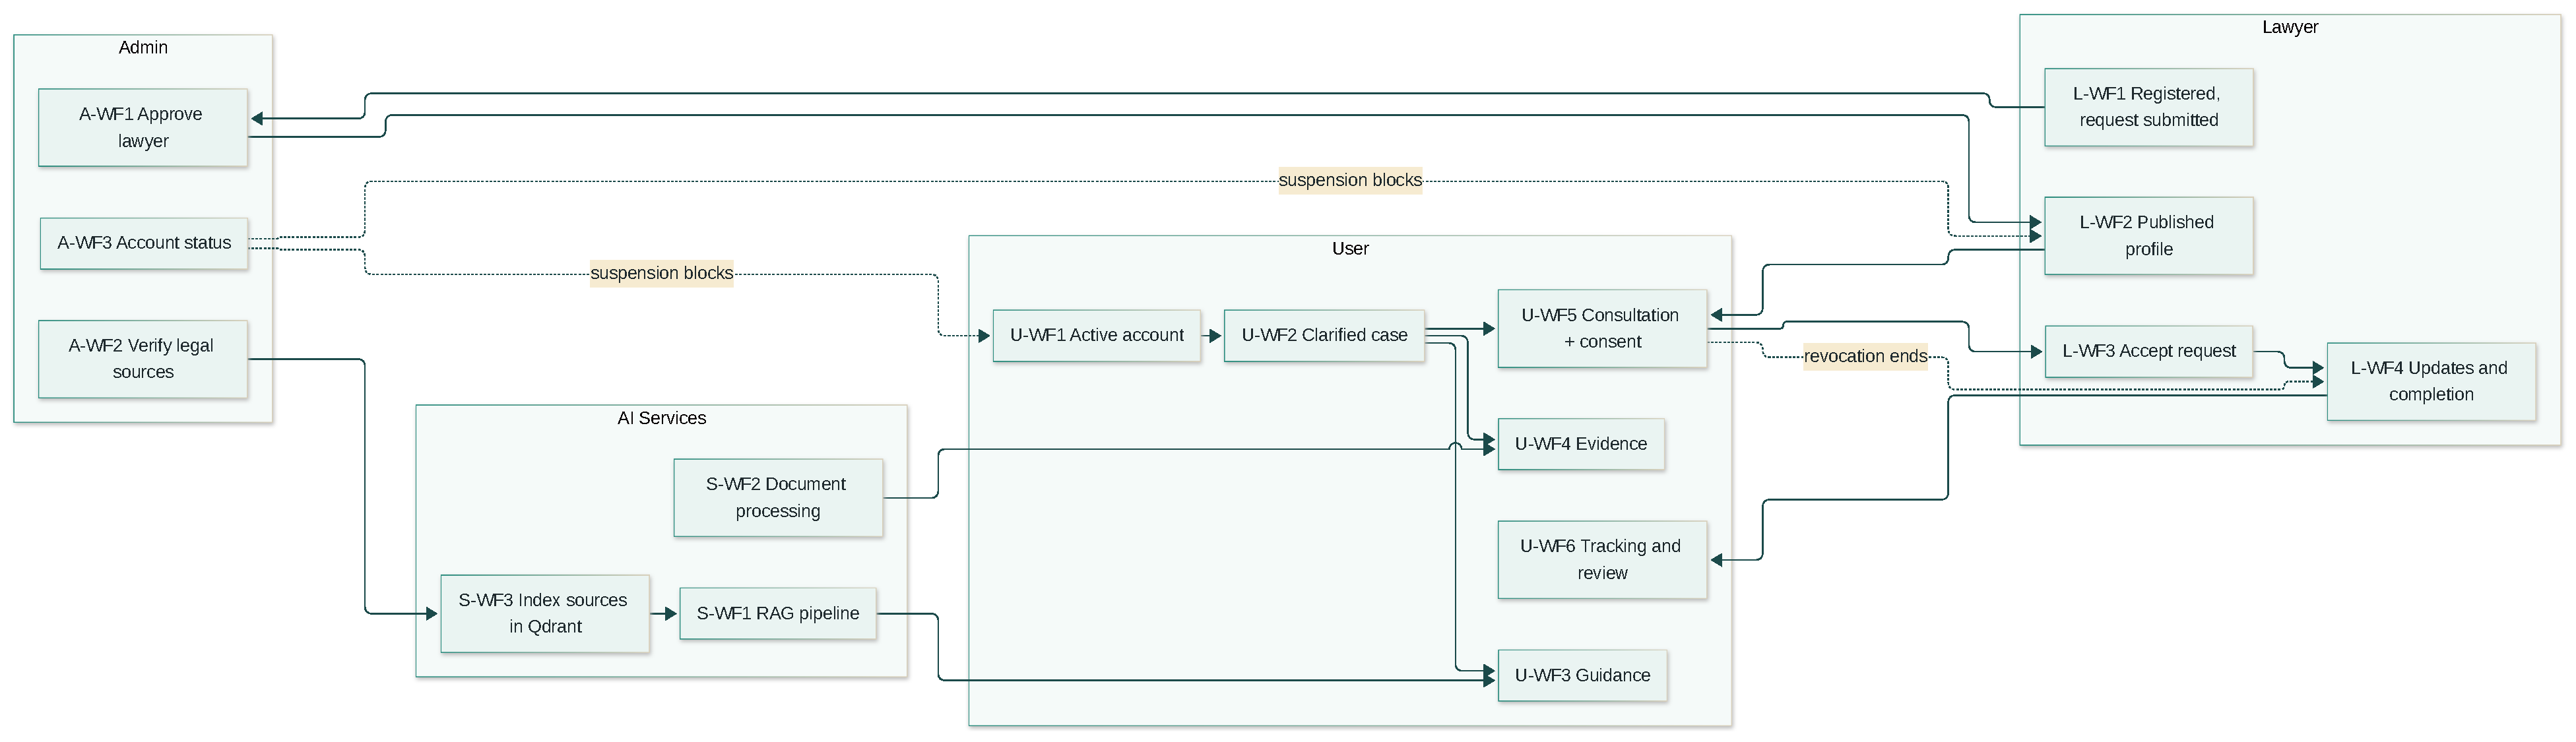
\includegraphics[width=24.5cm,height=14.8cm,keepaspectratio]{figures/dependency_graph.pdf}
\caption{Dependency graph between workflows and actors}\label{fig:6.1}
\end{figure}
\end{landscape}

\begin{longtable}{|L{3.54cm}|L{3.86cm}|L{2.42cm}|L{4.19cm}|}
\caption{Key dependencies}\label{tab:6.1}\\
\hline\headrow \thd{Dependent step} & \thd{Depends on} & \thd{Provided by} & \thd{If dependency is missing} \\ \hline
\endfirsthead
\hline\headrow \thd{Dependent step} & \thd{Depends on} & \thd{Provided by} & \thd{If dependency is missing} \\ \hline
\endhead
\hline\endlastfoot
AI guidance (U-WF3) & Verified and indexed legal sources & Admin (A-WF2) and System (S-WF3) & System returns ``no verified source'' and suggests a lawyer \\ \hline
AI guidance (U-WF3) & Case status Clarified & User (U-WF2) & Guidance is not offered until facts are complete \\ \hline
Evidence checklist (U-WF4) & Guidance generated or document uploaded & System (S-WF1, S-WF2) & Checklist is empty \\ \hline
Lawyer appears in directory (U-WF5) & Lawyer verification approved & Admin (A-WF1) & Lawyer is not listed \\ \hline
Consultation request (U-WF5) & Existing case, verified lawyer accepting requests & User, Lawyer (L-WF2) & Request button disabled \\ \hline
Lawyer reads case (L-WF3, L-WF4) & Active consent & User (U-WF5) & Access refused, request closed \\ \hline
Contact details released & Consultation accepted & Lawyer (L-WF3) & Contact details hidden \\ \hline
User messages lawyer (U-WF6) & Consultation accepted & Lawyer (L-WF3) & Messaging unavailable \\ \hline
Review (U-WF6) & Consultation Completed & Lawyer (L-WF4) & Review not allowed \\ \hline
Login (U-WF1, L-WF1) & Account not suspended & Admin (A-WF3) & Access refused \\ \hline
Notifications & Triggering event & System (S-WF4) & No notification sent \\
\end{longtable}

\section{Case Status Lifecycle}

% Mermaid source:
% %% name: state_case
% stateDiagram-v2
%     [*] --> Open : User creates case
%     Open --> Clarifying : Missing facts found
%     Clarifying --> Clarifying : Follow-up answered
%     Clarifying --> Clarified : All required facts known
%     Open --> Clarified : No facts missing
%     Clarified --> GuidanceReady : Cited answer generated
%     Clarified --> Clarified : No verified source
%     GuidanceReady --> SharedWithLawyer : Consultation requested with consent
%     SharedWithLawyer --> InProgress : Lawyer accepts
%     SharedWithLawyer --> GuidanceReady : Declined or consent revoked
%     InProgress --> GuidanceReady : Consent revoked
%     InProgress --> Resolved : User marks resolved
%     GuidanceReady --> Resolved : User marks resolved
%     Open --> Closed : User closes
%     Clarifying --> Closed : User closes
%     GuidanceReady --> Closed : User closes
%     Resolved --> [*]
%     Closed --> [*]
\begin{figure}[H]\centering
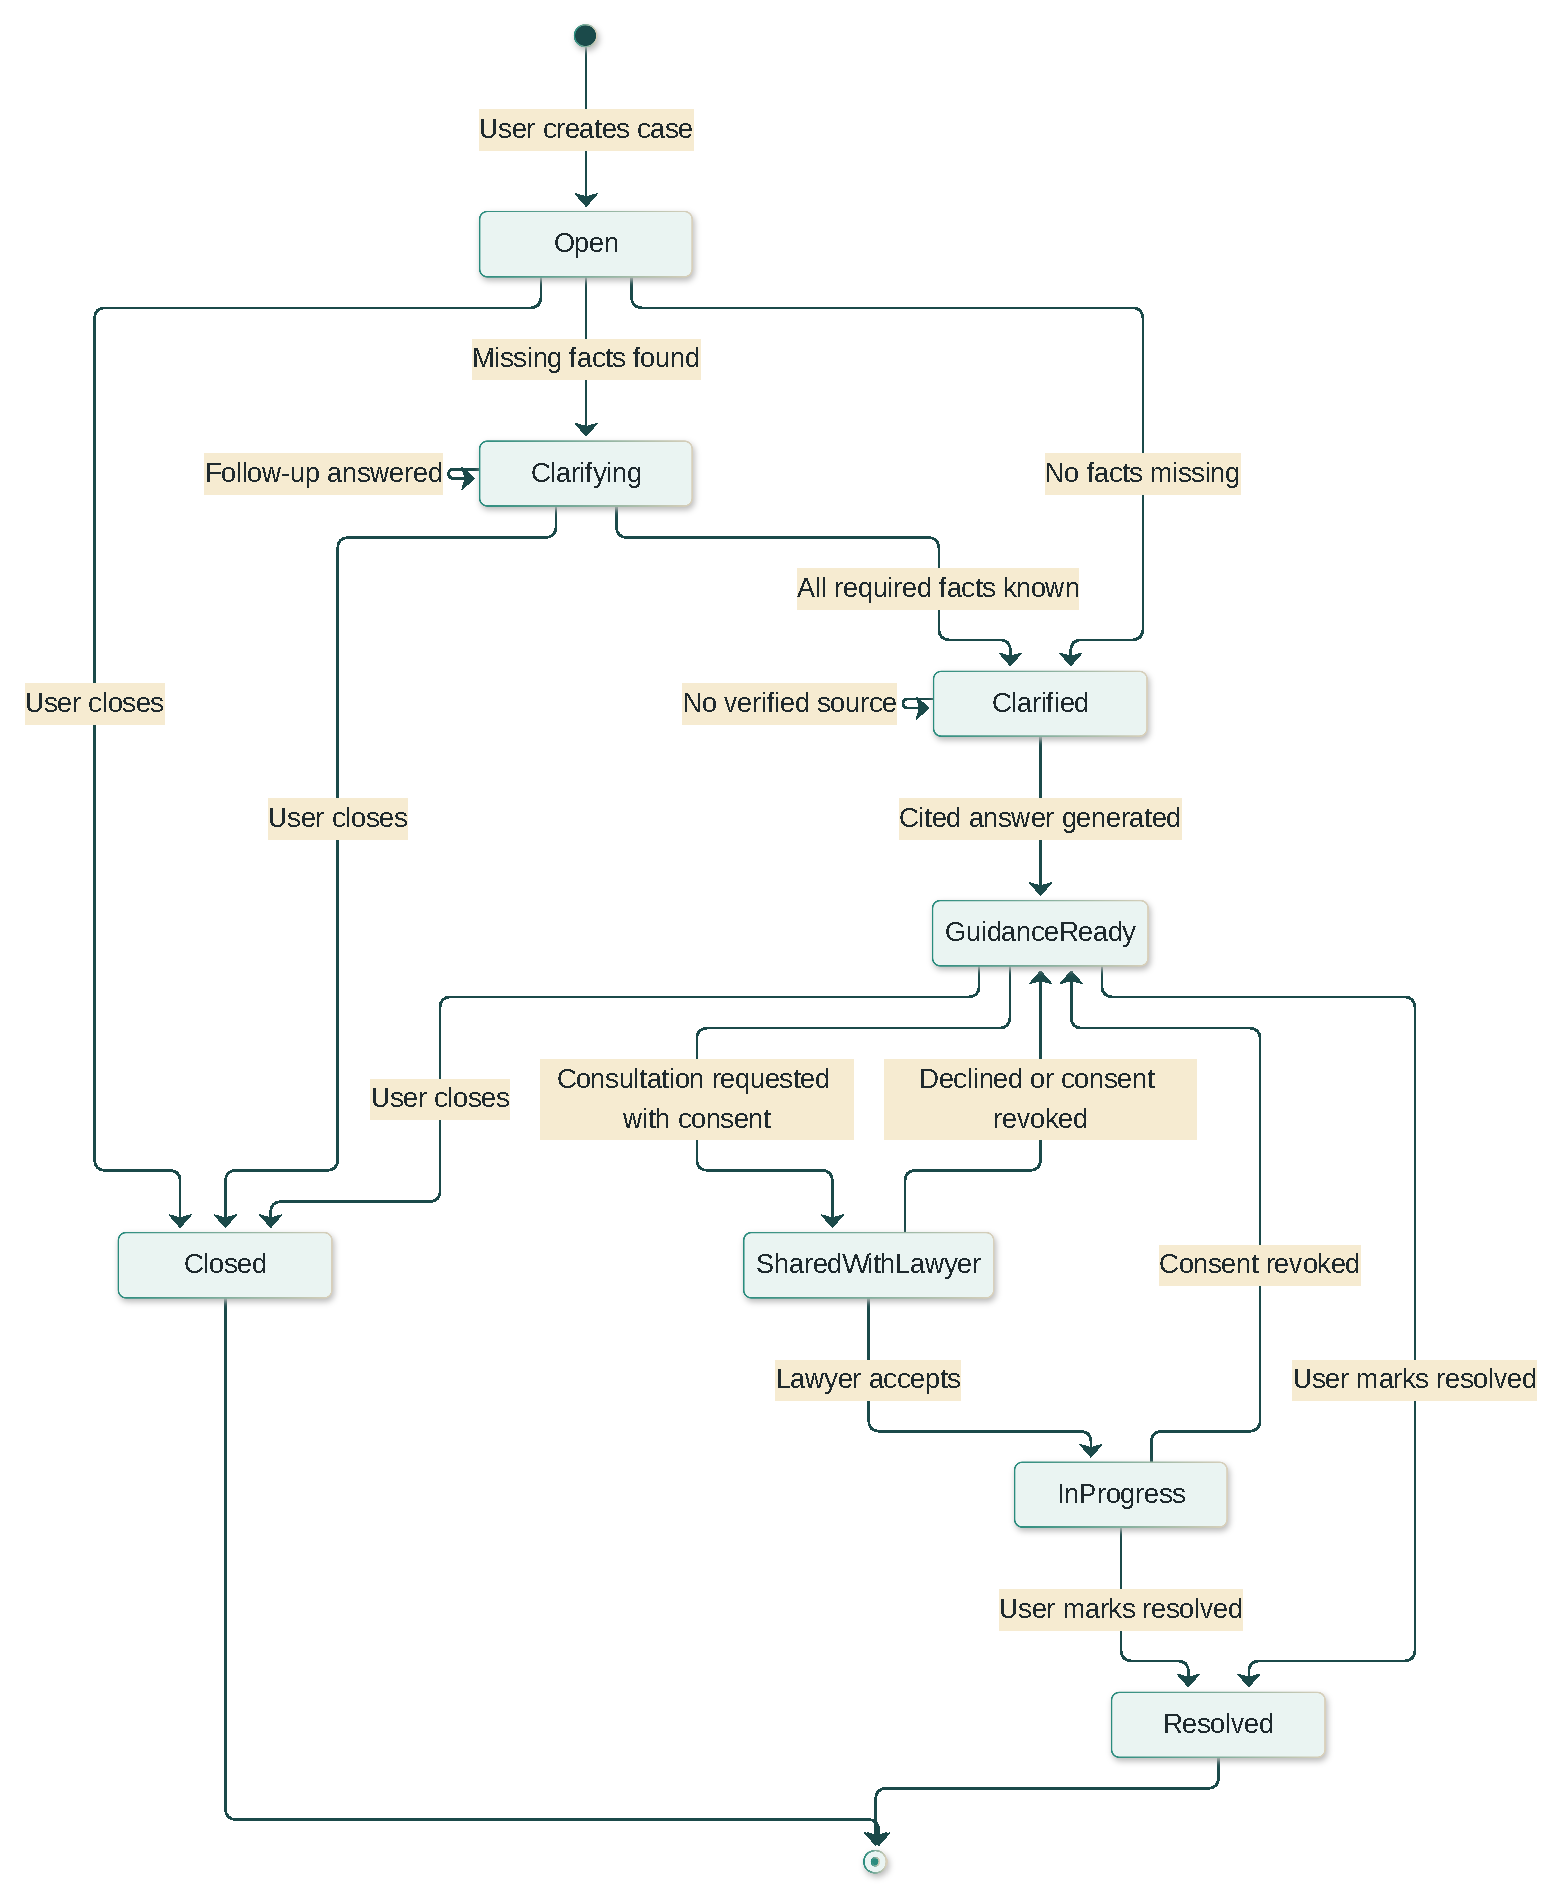
\includegraphics[width=\textwidth,height=0.80\textheight,keepaspectratio]{figures/state_case.pdf}
\caption{Case status lifecycle}\label{fig:6.2}
\end{figure}

\needspace{12\baselineskip}
\section{Consultation Status Lifecycle}

% Mermaid source:
% %% name: state_consult
% stateDiagram-v2
%     [*] --> Requested : User requests with consent
%     Requested --> Scheduled : Lawyer accepts
%     Requested --> Declined : Lawyer declines
%     Requested --> Rescheduling : Lawyer proposes another time
%     Rescheduling --> Scheduled : User accepts time
%     Rescheduling --> Cancelled : User rejects time
%     Requested --> Closed : Consent revoked
%     Scheduled --> Closed : Consent revoked
%     Scheduled --> Completed : Lawyer marks completed
%     Completed --> [*] : User may review
%     Declined --> [*]
%     Cancelled --> [*]
%     Closed --> [*]
\begin{figure}[H]\centering
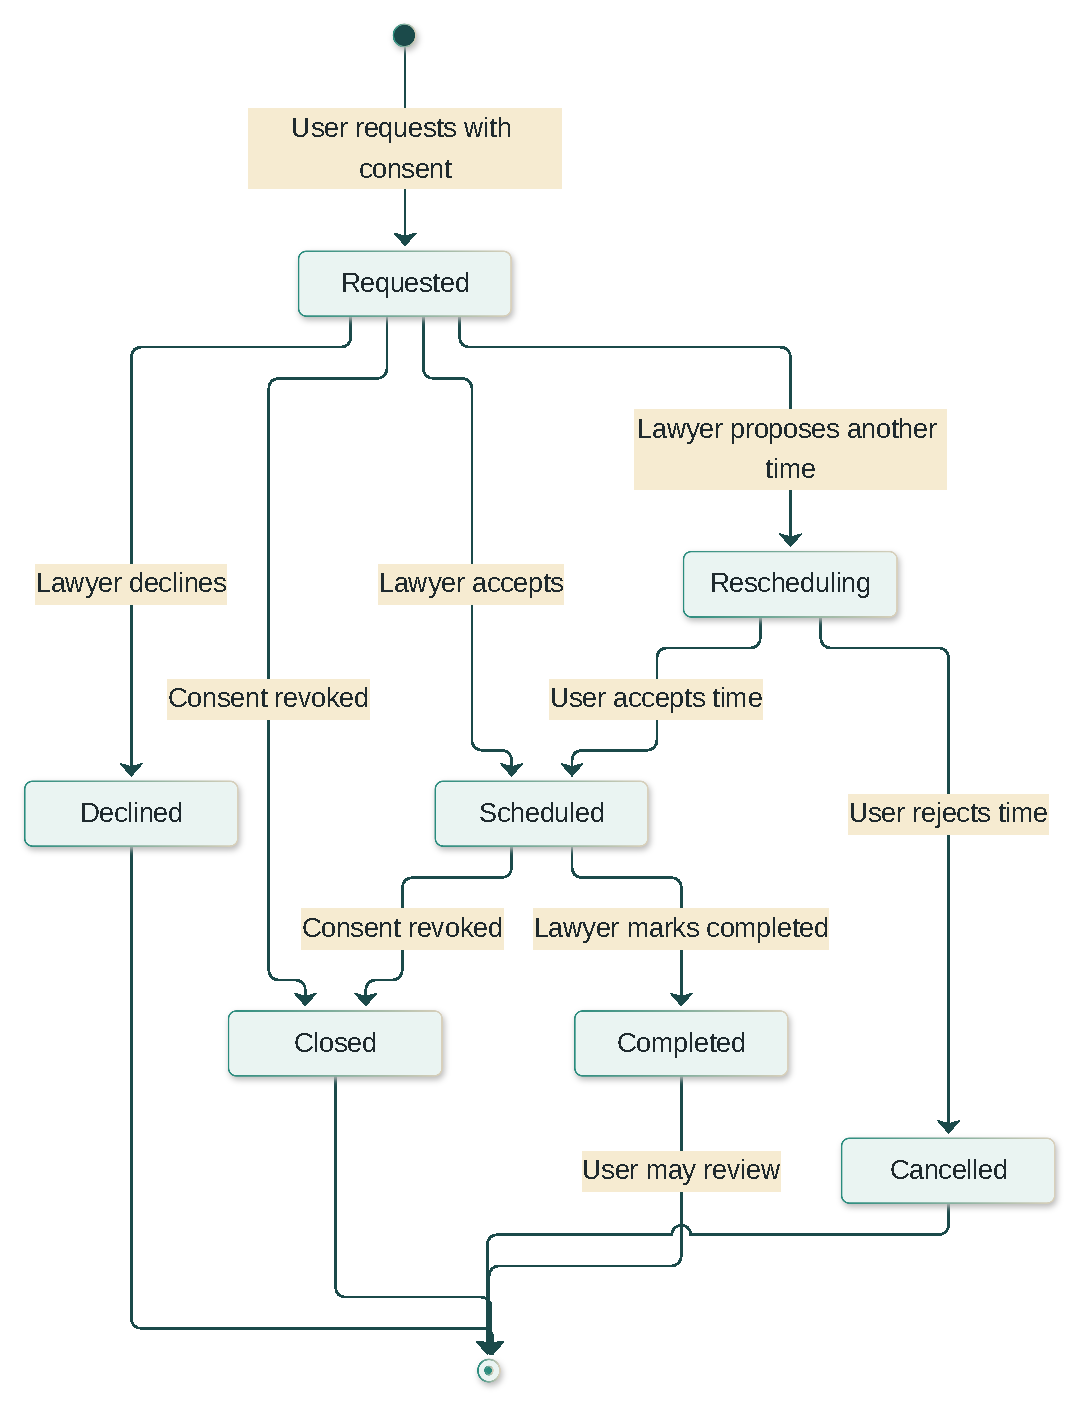
\includegraphics[width=\textwidth,height=0.80\textheight,keepaspectratio]{figures/state_consult.pdf}
\caption{Consultation status lifecycle}\label{fig:6.3}
\end{figure}

\needspace{12\baselineskip}
\section{Lawyer Verification Lifecycle}

% Mermaid source:
% %% name: state_lawyer
% stateDiagram-v2
%     [*] --> Unverified : Registers
%     Unverified --> Pending : Email verified, request submitted
%     Pending --> Verified : Admin approves
%     Pending --> Rejected : Admin rejects
%     Pending --> Pending : Admin requests information
%     Rejected --> Pending : Lawyer re-submits
%     Verified --> Pending : Bar details edited
%     Verified --> Suspended : Admin suspends
%     Suspended --> Verified : Admin reactivates
\begin{figure}[H]\centering
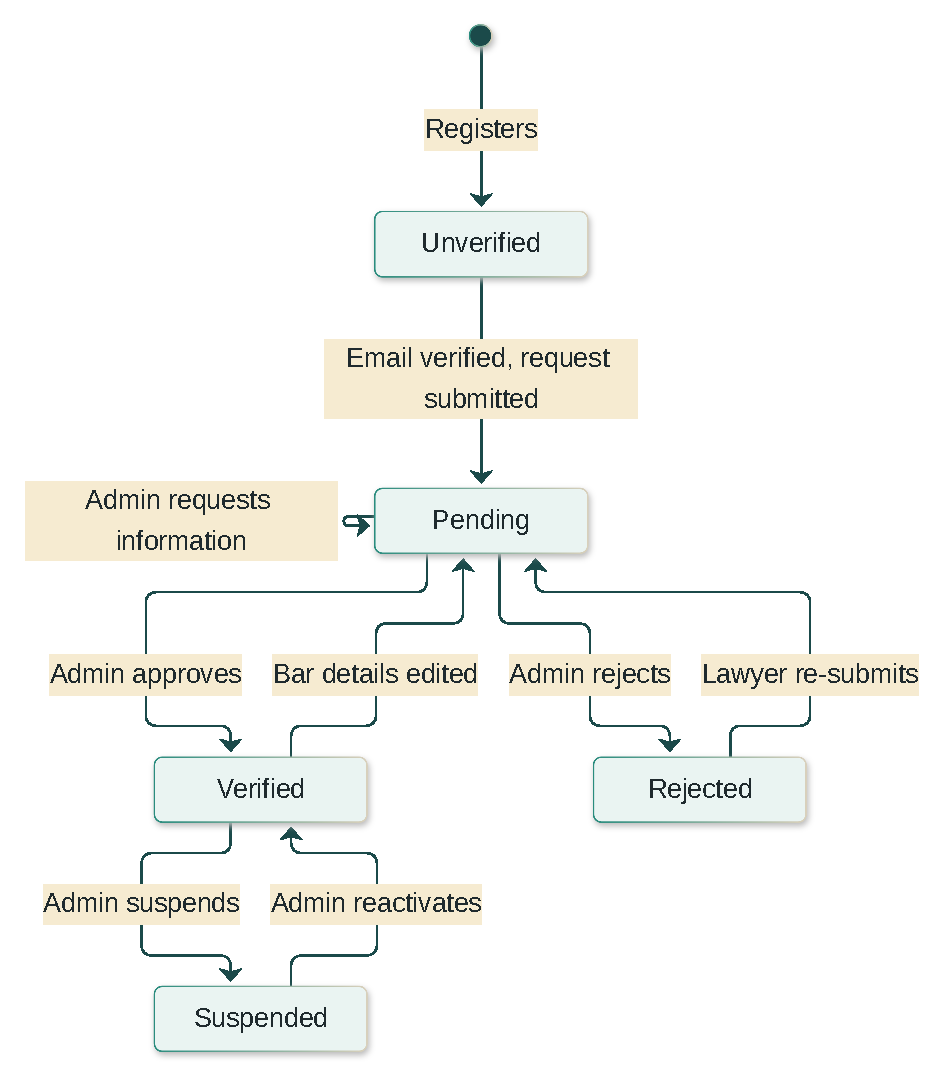
\includegraphics[width=\textwidth,height=0.80\textheight,keepaspectratio]{figures/state_lawyer.pdf}
\caption{Lawyer verification lifecycle}\label{fig:6.4}
\end{figure}

\needspace{12\baselineskip}
\section{Legal Source Lifecycle}

% Mermaid source:
% %% name: state_source
% stateDiagram-v2
%     [*] --> Processing : Admin uploads source
%     Processing --> AwaitingReview : Chunks indexed
%     AwaitingReview --> Processing : Chunks need correction
%     AwaitingReview --> Verified : Admin verifies
%     Verified --> Processing : Amended text re-indexed
%     Verified --> Retired : Source repealed
%     Retired --> [*]
\begin{figure}[H]\centering
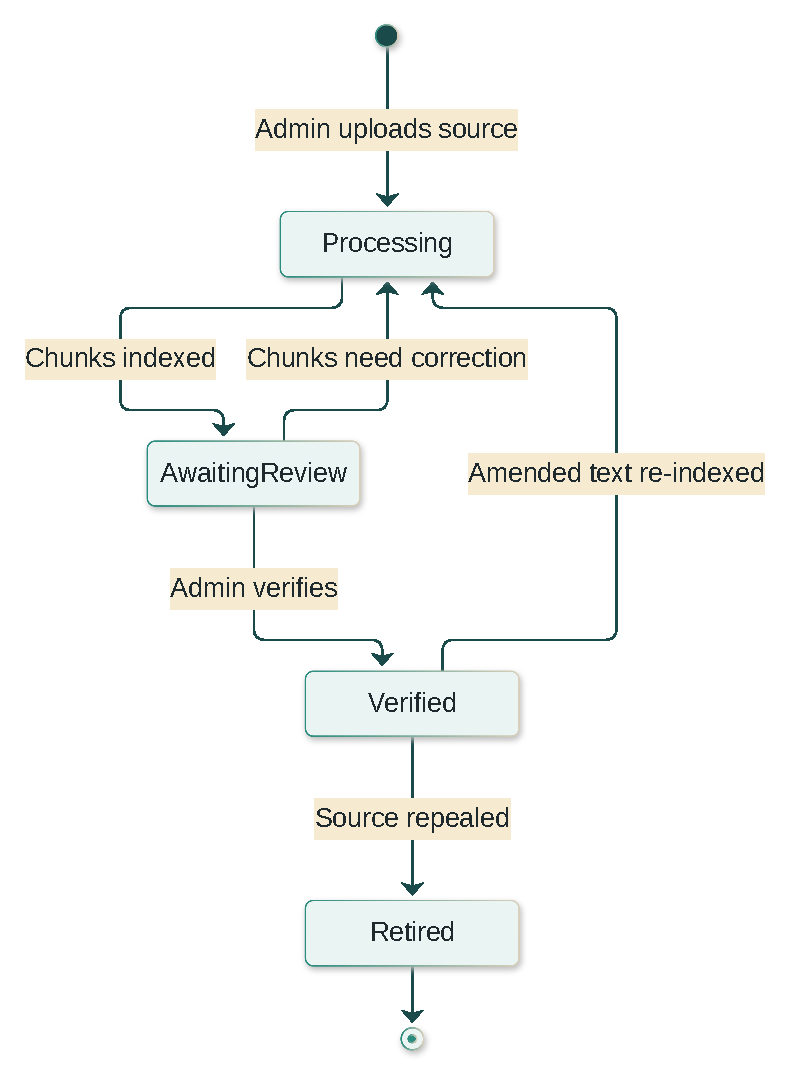
\includegraphics[width=\textwidth,height=0.80\textheight,keepaspectratio]{figures/state_source.pdf}
\caption{Legal source lifecycle}\label{fig:6.5}
\end{figure}

Only sources in the \textbf{Verified} state are retrievable by S-WF1. A \textbf{Retired} source is excluded from retrieval but kept so that earlier citations remain traceable.
